\NeedsTeXFormat{LaTeX2e}
\documentclass[a4paper,12pt,
headsepline,           % Linie zw. Kopfzeile und Text
oneside,               % einseitig
pointlessnumbers,      % keine Punkte nach den letzten Ziffern in Überschriften
bibtotoc,              % LV im IV
%DIV=15,               % Satzspiegel auf 15er Raster, schmalere Ränder   
%BCOR15mm               % Bindekorrektur
%,draft
]{scrartcl}

\usepackage{amsmath}
\usepackage{amsfonts}
\usepackage{amssymb}
\usepackage{enumitem}
\usepackage[utf8]{inputenc} % this is needed for umlauts
\usepackage[ngerman]{babel} % this is needed for umlauts
\usepackage[T1]{fontenc} 
\usepackage{commath}
\usepackage{xcolor}
\usepackage{booktabs}
\usepackage{float}
\usepackage{tikz-timing}
\usepackage{tikz}
\usepackage{multirow}
\usepackage[final]{pdfpages}
\usepackage{blindtext}
\usepackage{listings}
\usepackage[scaled]{helvet}
\usepackage{hyperref}
\usepackage{comment}
\usepackage{mathtools}
\DeclarePairedDelimiter{\ceil}{\lceil}{\rceil}

\usetikzlibrary{calc,shapes.multipart,chains,arrows}

\KOMAoptions{DIV=last} % Neuberechnung Satzspiegel nach Laden von Paket helvet

\usepackage{scrpage2}
\pagestyle{useheadings}

\renewcommand{\familydefault}{\sfdefault} 

\setlength{\parindent}{0pt}   % kein linker Einzug der ersten Absatzzeile
\setlength{\parskip}{1.4ex plus 0.35ex minus 0.3ex} % Absatzabstand, leicht variabel

\newcommand{\fullname}{Gruppe 10}
\newcommand{\titel}{Softwaregrundprojekt Meilenstein 4}
\newcommand{\jahr}{2019}
\newcommand{\dozent}{Florian Ege}
\newcommand{\betreuer}{Stefanos Mytilineos}
\newcommand{\fakultaet}{Ingenieurwissenschaften, Informatik und\\Psychologie}
\newcommand{\institut}{Institut für Softwaretechnik und Programmiersprachen}

\pdfinfo{
    /Author (\fullname)
    /Title (\titel)
    /Producer     (pdfeTex 3.14159-1.30.6-2.2)
    /Keywords ()
}

\hypersetup{
    pdftitle=\titel,
    pdfauthor=\fullname,
    pdfsubject={Softwaregrundprojekt-Abgabe},
    pdfproducer={pdfeTex 3.14159-1.30.6-2.2},
    colorlinks=false,
    pdfborder=0 0 0	% keine Box um die Links!
}

% Trennungsregeln
\hyphenation{Sil-ben-trenn-ung}

\makeatletter
\@addtoreset{section}{part}
\makeatother

\newcommand{\begriff}[7] {
	\begin{table}[H]
		\centering
		\begin{tabular}{|p{2,5cm}|p{12cm}|}
			%\hline
			%\toprule \\
			\hline
			\textbf{Begriff} & \textbf{#1} \\ \hline
			%\midrule \\
			\textbf{Beschreibung} & #2 \\ \hline
			%\midrule
			\textbf{Ist-ein} & #3 \\ \hline
			%\midrule
			\textbf{Kann-sein} & #4 \\ \hline
			%\midrule
			\textbf{Aspekt} & #5 \\ \hline
			%\midrule
			\textbf{Bemerkung} & #6 \\ \hline
			%\midrule
			\textbf{Beispiel} & #7 \\ %\hline
			%\bottomrule
			\hline
		\end{tabular}
	\end{table}
}

\newcommand{\anf}[7] {
    \begin{table}[H]
        \centering
        \begin{tabular}{|p{3.2cm}|p{11.3cm}|}
        	\hline
            \textbf{ID:} & \textbf{#1} \\ \hline
            \textbf{Titel:} & #2 \\ \hline
            \textbf{Beschreibung:} & #3 \\ \hline
            \textbf{Begründung:} & #4 \\ \hline
            \textbf{Abhängigkeiten:} & #5 \\ \hline
            \textbf{Priorität:} & #6 \\ \hline
            \textbf{Akteure:} & #7 \\ \hline
        \end{tabular}
    \end{table}
}

\newcounter{fanfCount}
\newcommand{\fanf}[6] {
    \stepcounter{fanfCount}
    \anf{FA\thefanfCount}{#1}{#2}{#3}{#4}{#5}{#6}
}
\newcounter{qanfCount}
\newcommand{\qanf}[6] {
    \stepcounter{qanfCount}
    \anf{QA\theqanfCount}{#1}{#2}{#3}{#4}{#5}{#6}
}

\newcommand{\akt}[4] {
    \begin{table}[H]
        \centering
        \begin{tabular}{|p{3cm}|p{11.5cm}|}
        	\hline
            \textbf{ID:} & \textbf{#1} \\ \hline
            \textbf{Titel:} & #2 \\ \hline
            \textbf{Beschreibung:} & #3 \\ \hline
            \textbf{Rolle:} & #4 \\ \hline
        \end{tabular}
    \end{table}
}

\newcounter{faktCount}
\newcommand{\fakt}[3] {
    \stepcounter{faktCount}
    \akt{AKT\thefaktCount}{#1}{#2}{#3}
}

\begin{document}
    \thispagestyle{empty}
    \begin{addmargin*}[4mm]{-10mm}

        
\includegraphics[height=1.8cm]{images/unilogo_bild}
        \hfill
        
\includegraphics[height=1.8cm]{images/unilogo_wort}\\[1em]

        {\footnotesize
        %{\bfseries Universität Ulm} \textbar ~89069 Ulm \textbar ~Germany
        \hspace*{115mm}\parbox[t]{35mm}{\bfseries Fakultät für\\
        \fakultaet\\
        \mdseries \institut}\\[2cm]

        \parbox{140mm}{\bfseries \LARGE \titel}\\[2.5em]
        {\footnotesize Softwaregrundprojekt an der Universität Ulm}\\[3em]

        {\footnotesize \bfseries Vorgelegt von:}\\
        {\footnotesize \fullname\\}\\ [1em]
        {\footnotesize \bfseries Dozent:}\\
        {\footnotesize \dozent\\}\\[1em]
        {\footnotesize \bfseries Betreuer:}\\
        {\footnotesize \betreuer}\\ [1em]
        {\footnotesize \jahr}
        }
    \end{addmargin*}
    \pagebreak
    \tableofcontents
    \pagebreak

    \part{Überblick}
    \subsection{Einleitung}
Bei dem Projekt handelt es sich um die Konzeption und Implementierung eines online Multiplayer-Spiels aus der Welt von Harry Potter – genauer: \textit{Fantastic Feasts}. Es ist eine rundenbasierte Form des bekannten Spiels Quidditch.


Im Mittelpunkt des Projekts steht das Erlernen von Fähigkeiten im Umgang mit einem größeren Softwareprojekt. Es werden keine kommerziellen Ziele verfolgt.

Der Auftraggeber – im weitesten Sinne die Universität Ulm – verfolgt das Ziel, den Studenten Fähigkeiten zu vermitteln und sie anschließend nach genau definierten Maßstäben zu bewerten. Zu diesen Fähigkeiten gehört folgendes:

Zunächst einmal stehen Planen, Formulieren von Anforderungen und Modellierung von Software an. Es folgt die Auseinandersetzung mit verschiedenen Plattformen und Technologien auf die für die Implementierung zurückgegriffen werden soll. Gleichzeitig wird das Ziel verfolgt, übergeordnete Fähigkeiten zur Qualitätssicherung, zur Versionenverwaltung oder zu agilen Entwicklungsprozessen im Team zu erwerben. 
Erst dann kommen praktische Programmierfähigkeiten zum tragen. Auch hier ist es das Ziel, diese auszubauen.

Die Studierenden – in diesem Fall 6 Studenten der Informationssystemtechnik – verfolgen das Ziel, das Projekt nach den Anforderungen im Lastenheft erfolgreich umzusetzen und die Abnahmeprüfung zu bestehen.





\subsection{Motivation}
Die Motivation für das Projekt lässt sich – wie bei den Zielen – in die der Universität und die der Studenten aufteilen.

Die Universität gibt die Inhalte vor. Diese sollen von den Studenten bestmöglich erlernt werden, da es Teil ihrer Ausbildung darstellt. Die Universität will somit ihrem Auftrag der Lehre gerecht werden.
 

Für die Studenten ist die Motivation der Erwerb und Ausbau der oben genannten Fähigkeiten und im weitesten Sinne eine erfolgreiche Ausbildung in ihrem Fach. Zusätzlich soll ein Spiel entwickelt werden, das funktioniert und Spaß macht.
 

\subsection{Vision}
Das fertige System soll folgendermaßen aufgebaut sein: Einer Client-Server-Architektur folgend kommunizieren ein oder mehrere Clients mit dem Server, auf dem die Spiellogik läuft. Die Spieler haben client-seitig eine ansprechende und lebendige GUI, über die sie \textit{Fantastic Feasts} spielen, eine Partie als Zuschauer verfolgen, Charaktere und Ausrüstung zu Teams mitsamt Farben und Logo zusammen stellen können und die Möglichkeit haben, Partien zu konfigurieren. Begleitet wird die visuelle Darstellung von Soundeffekten und einer thematisch Ansprechenden Spielmusik.

Im durch und durch taktischen Spiel mit zwei sich genüberstehenden Quidditch-Teams können die Spieler Runde für Runde Spielfiguren auf Besen über das Spielfeld jagen lassen, Punkte erzielen, den Gegner sabotieren und Publikumseffekte zu ihrem Vorteil einsetzen. Doch selbst bei noch so guter Taktik kann ihnen der Zufall einen Strich durch die Rechnung machen, da nicht immer alles so eintritt, wie es sich die einzelnen Spieler vielleicht erhofft haben.

Was die Spielmodi betrifft, ist das Kern-Szenario das Multiplayer-Spiel. Hier entsteht durch den Wettstreit zweier Spieler die größte Spannung. Doch um das Spiel auch alleine spielbar zu machen, existiert ein Singleplayer-Modus. Eine ausgefeilte KI mit voraussichtlich mehreren Schwierigkeitsstufen stellt für Einzelspieler eine spannende Herausforderung dar. Wer sich noch auf den großen Wettkampf vorbereitet, die Taktik andere Spieler erlernen will oder einfach Spaß am Zuschauen hat, kann sich im Zuschauer-Modus in andere Multiplayer-Partien einklinken. Damit bleibt einer breiten Zielgruppe an Spielern kaum etwas zu wünschen übrig.

\subsection{Projektkontext}
Auftraggeber des Projektes ist die Servicegruppe Informatik der Universität Ulm, die das Modul Softwaregrundprojekt veranstaltet. Der Tutor Stefanos Mytilineos vertritt den Auftraggeber während der Projektlaufzeit, in höherer Instanz ist Florian Ege verantwortlich. Als weiterer Stakeholder tritt das Team auf, das das Projekt letztendlich entwickelt. Es besteht aus sechs Studenten der Informationssystemtechnik: Tarik Enderes, Tim Luchterhand, Jonas Merkle, Paul Nykiel, Björn Petersen und Michael von Hohnhorst. Diese bearbeiten das Projekt nicht in Vollzeit, da sie parallel den weiteren Verlauf ihres Studiums verfolgen. 

Indirekt am Entwicklungsprozess beteiligt ist das Standardisierungskomitee, in das auch aus diesem Team ein Vertreter geschickt wird. Dort werden alle nötigen Protokolle und Schnittstellen definiert, die bei der Entwicklung von \textit{Fantastic Feasts} benötigt werden. Weitere Stakeholder, die jedoch erst später in Erscheinung treten, sind andere Teams, die gegebenenfalls auf einen Komponenten dieses Projektes angewiesen sind. Sie werden auf einer bevorstehenden Messe zu potenziellen Kunden. In ihrem Interesse liegt eine saubere Implementierung bei gleichzeitig guter Dokumentation des Komponenten. Zu guter letzt muss dieses Projekt sowie die Einzelleistung eines jeden Team-Mitgliedes die Prüfer in der Abnahmeprüfung überzeugen – sie stellen so gesehen die wichtigsten Kunden dar.

Da bei der Implementierung auf den agilen Entwicklungsprozess Scrum zurückgegriffen wird, sollen auch hier die Rollen kurz benannt werden. In dieser Phase übernimmt der oben genannte Tutor die Rolle des Product Owners. Der ScrumMaster wird innerhalb des oben genannten Teams ernannt.

Folgeprojekte von \textit{Fantastic Feasts} sind derzeit nicht vorgesehen. Denkbar wäre jedoch ein Publishing des Spiels mit ständig laufendem Server und beliebig vielen Server-Instanzen – so könnte \textit{Fantastic Feasts} weltweit von zahlreichen Spielern gespielt werden.

    \part{Anforderungsanalyse} 
    \section{Fachwissen}
    \begriff{Nutzer}
{Ein Mensch, der einen Rechner bedient und entweder den Client zum Spielen des Spiels oder zur Beobachtung einer Partie benutzt, oder den Team-Editor bedient. Jeder Benutzer hat einen Nutzernamen, mittels dem er von anderen Nutzern erkannt werden kann.}
{-}
{Spieler, Gast}
{Zur Beschreibung des Programmverlaufs}
{-}
{JägerMaister69}

\begriff{Spieler}
{Ein Nutzer, der das Computerspiel \glqq{}Fantastic Feasts\grqq{}  spielt.}
{Nutzer}
{-}
{Zur Beschreibung des Programmverlaufs}
{-}
{-}

\begriff{Gast}
{Ein Nutzer, der eine laufende Partie beobachtet}
{Nutzer}
{-}
{Zur Beschreibung des Programmverlaufs}
{-}
{-}

\begriff{Client}
{Das Computerprogramm, das mit einer grafischen Oberfläche ausgestattet ist und einem Nutzer erlaubt, eine Verbindung mit einem Server herzustellen und damit zu Kommunizieren}
{-}
{-}
{Zum Spielen des Spiels \glqq{}Fantastic Feasts\grqq{} }
{Der Begriff bezieht sich nicht auf den Menschen, der das Programm bedient}
{-}

\begriff{Server}
{Die zentrale Komponente, in dem die Spiellogik implementiert ist und die Programmbefehle abwickelt und mit dem sich Clients verbinden können, um eine Partie zu spielen oder zu beobachten. Die Kommunikation erfolgt mit JSON}
{-}
{-}
{Ist für die Kommunikation von Clients, für das Verwalten des Spielgeschehens, Ressourcenverwaltung und die Spiellogik verantwortlich.}
{-}
{-}

\begriff{Team-Editor}
{Ermöglicht einem Nutzer mit einer grafischen Oberfläche, ein eigenes Team zu erstellen und zu bearbeiten. Die Einstellungen werden danach als JSON-Datei gespeichert.}
{-}
{-}
{Zur Erstellung von nutzereigenen Teams.}
{-}
{-}

\begriff{KI-Client}
{Meldet sich beim Server wie ein normaler Client an und simuliert mit einer KI einen menschlichen Spieler. Hat keine grafische Oberfläche. Meldet sich mit dem Nutzernamen \glqq{}KI\grqq{}  ein.}
{-}
{-}
{Zum Spielen gegen einen Computergegner}
{-}
{-}

\begriff{KI}
{Definiert die Regeln, nach denen der KI-Client auf die durch den Server vermittelten Geschehen im Spiel reagiert.}
{-}
{-}
{Zum Spielen gegen einen Computergegner}
{Die KI ist die Logik, nach der der Computer das Spiel spielt und kein Programm}
{-}

\begriff{Spielfeld}
{Ein grafisch darstellbares Raster, auf dem sich die Spielfiguren bewegen}
{-}
{-}
{Dient als virtuelles Spielbrett mit klar definierten Abgrenzungen}
{Wird nicht Spielumgebung genannt um Verwechslung mit dem Client zu vermeiden}
{-}

\begriff{Zelle}
{Die kleinste Einheit des Spielfeldes, also ein Quadrat davon}
{-}
{Zentrumszelle, Torring, Hüterzonenzelle}
{Mögliche Standorte der Spielfiguren}
{Wird nicht Feld genannt, da das ein eher vager Begriff ist}
{-}

\begriff{Zentrum}
{Der 3x3 Zellen große Abschnitt in der Mitte des Spielfeldes}
{-}
{-}
{Summe aller Zentrumszellen}
{Ist das Mittelfeld im Lastenheft}
{-}

\begriff{Hüterzone}
{Die Bereiche am linken und rechten Rand des Spielfeldes, in dem sich die Torringe befinden}
{-}
{-}
{Summe aller kritischen Zellen und Torring}
{-}
{-}

\begriff{Torring}
{Die Zellen in die beide Teams den Quaffel bewegen wollen. Es wird zwischen eigenen und gegnerischen Torringen unterschieden.}
{Zelle}
{Eigener Torring, Gegnerischer Torring}
{Hauptquelle von Punkten}
{Torring im Lastenheft}
{}

\begriff{Zentrumszelle}
{Eine Zelle im Zentrum des Spielfeldes (siehe Zentrum)}
{Zelle}
{-}
{Startpunkt für Quaffel und Klatscher}
{-}
{-}

\begriff{Hüterzonenzelle}
{Eine Zelle in einem kritischen Bereich des Spielfeldes}
{Zelle}
{-}
{limitierendes Element für das Abliefern der Quaffel}
{-}
{-}

\begriff{Spielobjekt}
{Jedes Objekt, das sich auf dem Spielfeld befindet und darauf bewegt werden kann}
{-}
{Ball, Spielfigur}
{-}
{Nicht zu verwechseln mit Spielfigur}
{-}

\begriff{Ball}
{Ein Spielobjekt, das nicht direkt, nur indirekt von einem Spieler beeinflusst werden kann}
{Spielobjekt}
{Quaffel, Klatscher, Schnatz}
{Festpunkte zur Steuerung des Spielverlaufs}
{-}
{-}

\begriff{Spielfigur}
{Ein Spielobjekt, das von einem Spieler direkt gesteuert wird. Jede Spielfigur hat einen Namen, einen Besenrang, ein Geschlecht, ein Team und eine Rolle. Man unterscheidet außerdem zwischen eigenen und gegnerischen Spielfiguren.}
{Spielobjekt}
{Hüter, Sucher, Jäger, Treiber}
{Mitglieder eines Teams}
{Spieler im Lastenheft}
{Name: Luke Skywalker, Rolle: Hüter des Teams \glqq{}Jedi\grqq{}, Geschlecht: männlich, Besenrang: 5}

\begriff{Quaffel}
{Passives Objekt, mit dem Jäger und Hüter interagieren können und von ihnen nach Möglichkeit in ein gegnerisches Zielfeld befördert werden soll.}
{Ball}
{-}
{Zentrales Spielobjekt}
{-}
{-}

\begriff{Klatscher}
{Ball, der sich von selbst auf Spielfiguren zubewegt, die keine Treiber sind und diese betäuben können und von Treibern bewegt werden können.}
{Ball}
{-}
{Zusätzliches taktisches Spielelement}
{-}
{-}

\begriff{Schnatz}
{Ball, der von den Suchern gejagt wird und deren Fund die Partie beendet}
{Ball}
{-}
{Definiert Spielende}
{\glqq{}Schnatz\grqq{}  im Lastenheft}
{-}

\begriff{Partie}
{Ein einzelnes Spiel. Beginnt beim Platzieren der Figuren und endet mit dem Bestimmen des Gewinners.}
{-}
{-}
{Beschreibung des Spielablaufs}
{-}
{Spieler VodkaVodka98 spielt gegen Spieler LongEiländ}

\begriff{Hüter}
{Spielfigur, deren Aufgabe es ist, den Quaffel von den eigenen Zielfeldern fernzuhalten}
{Spielfigur}
{Eigener Hüter, Gegnerischer Hüter}
{Letzte Verteidigungslinie}
{-}
{Siehe \glqq{}Spielfigur\grqq{} }

\begriff{Sucher}
{Spielfigur, die den Schnatz jagt}
{Spielfigur}
{Eigener Sucher, Gegnerischer Sucher}
{Beendet die Partie}
{-}
{Darth Vader, gegnerischer Sucher, Besenrang 2}

\begriff{Jäger}
{Spielfigur, die den Quaffel in ein einen gegnerischen Torring befördern soll}
{Spielfigur}
{Eigener Jäger, Gegnerischer Jäger}
{Holt Punkte für das eigene Team}
{\glqq{}Jäger\grqq{}  im Lastenheft. Jäger beschreibt die Rolle der Spielfigur aber besser.}
{Han Solo, eigener Jäger, Besenrang 3}

\begriff{Treiber}
{Spielfigur, mit der der Spieler eigene Spielfiguren vor Klatschern schützt und gegnerische damit abschießen kann}
{Spielfigur}
{Eigener Treiber, Gegnerischer Treiber}
{Interagiert mit Klatschern}
{-}
{Boba Fett, gegnerischer Treiber, Besenrang 4}

\begriff{Geschlecht}
{Jede Spielfigur ist entweder männlich oder weiblich.}
{-}
{-}
{Team-Editierung}
{-}
{-}

\begriff{Team}
{Die Menge aller Spielfiguren auf dem Spielfeld, die von einem einzigen Spieler kontrolliert wird. Ein Team hat einen Namen, ein Motto, ein Logo, eine Hauptfarbe und eine Ersatzfarbe.}
{eigenes Team, gegnerisches Team}
{-}
{Beschreibung einer Partie}
{-}
{Galaktisches Imperium, Motto: \glqq{}Unbegrenzte MAAACHT!\grqq{}, [Todesstern als Logo], Hauptfarbe: Schwarz, Ersatzfarbe: Rot }

\begriff{Punkte}
{Der Spieler mit mehr Punkten am Ende der Partie gewinnt. Werden durch das Platzieren des Quaffel in einem gegnerischen Torring oder das Finden des Schnatzes erhalten.}
{-}
{-}
{Bestimmung des Gewinners}
{-}
{SchnapsNase hat 20 Punkte}

\begriff{Besetzen}
{Eine Spielfigur besetzt das Feld, auf dem sie sich befindet}
{-}
{-}
{Beschreibung des Spielgeschehens}
{Zwei Spielfiguren können sich nicht auf derselben Zelle befinden}
{Chewbacca besetzt Zelle 5:3}

\begriff{Besenrang}
{Jede Spielfigur hat einen Besenrang von 1 bis 5, der die Wahrscheinlichkeit bestimmt, dass sie noch einmal ziehen kann. Besenrang 1 ist der beste.}
{-}
{-}
{Unterscheidet Qualität der Spielfiguren.}
{Ersetzt die verschiedenen \glqq{}Besen\grqq{} aus dem Lastenheft mit einer Skala von 1 bis 5 zur besseren Übersicht.}
{Yoda hat Besenrang 1.}

\begriff{Aktion}
{Jede durch einen Spieler hervorgerufene Änderung der Spielsituation}
{-}
{Ziehen, Schießen, Schlagen, Einmischung, Übernahme}
{Weiterführung der Partie}
{-}
{Obi-Wan Kenobi zieht von Zelle 8:7 auf Zelle 9:7}

\begriff{Ziehen}
{Die Bewegung einer Spielfigur von einer Zelle auf eine andere durch direkten Befehl des Spielers}
{Aktion}
{-}
{Beschreibung des Spielverlaufs}
{Bezieht sich nicht auf erzwungene Bewegungen einer Spielfigur.}
{Obiwan Kenobi zieht von Zelle 8:7 auf Zelle 9:7}

\begriff{Befördern}
{Bewegen des Quaffel mittels einer Spielfigur}
{-}
{-}
{Bewegen des Quaffel, allgemeiner Begriff}
{Keine Aktion, da eventuell eine passive Folge, z.B. durch Ziehen}
{-}

\begriff{Schießen}
{Die Bewegung des Quaffel durch einen Hüter oder Jäger auf eine andere, entfernte Zelle ohne Bewegung der Spielfigur}
{Aktion}
{-}
{Bewegung des Quaffel um mehrere Felder}
{\glqq{}Werfen\grqq{}  im Lastenheft. Analog zum Schussvektor benannt.}
{Mace Windu schießt den Quaffel auf Zelle 10:4}

\begriff{Schlagen}
{Die erzwungene Bewegung eines Klatschers durch einen Treiber}
{Aktion}
{-}
{Interaktion mit Klatschern}
{\glqq{}Kloppen\grqq{}  im Lastenheft}
{R2-D2 schlägt einen Klatscher auf Zelle 5:10}

\begriff{Einmischung}
{Hilfsfähigkeiten, die nicht von Spielobjekten ausgehen. Werden von einem Spieler gesteuert. Bei jeder Benutzung besteht eine Chance, dass die verwendete Einmischung bis zum Ende der Partie für den jeweiligen Spieler vom Schiedsrichter deaktiviert werden.}
{Aktion}
{Teleportation, Fernangriff, Impuls, Schnatzjagd}
{Zusätzliche taktische Element}
{Ersetzt die \glqq{}Fans\grqq{}  aus dem Lastenheft}
{Lando Calrissian wird auf Zelle 6:6 teleportiert}

\begriff{Teleportation}
{Einmischung, die eine Spielfigur auf eine zufällige Zelle teleportiert}
{Einmischung}
{-}
{-}
{Ersetzt \glqq{}Elfen\grqq{}  aus Lastenheft}
{Siehe \glqq{}Einmischungen\grqq{} }

\begriff{Fernangriff}
{Trifft eine gegnerische Spielfigur. Ziel verliert gegebenenfalls den Quaffel und wird auf eine zufällige benachbarte, freie Zelle bewegt.}
{Einmischung}
{-}
{-}
{Statt \glqq{}Kobolde\grqq{}  im Lastenheft}
{Jango Fett wird von Fernangriff auf Zelle 5:6 gestoßen}

\begriff{Impuls}
{Wenn eine Spielfigur den Quaffel hält, wird sie bei Benutzung verloren}
{Einmischung}
{-}
{-}
{Statt \glqq{}Trolle\grqq{}  im Lastenheft}
{C-3PO verliert wegen eines Impuls den Quaffel}

\begriff{Schnatzstoß}
{Bewegt den Schnatz in eine zufällige Richtung um ein Feld}
{Einmischung}
{-}
{-}
{\glqq{}Schnatzschnappen\grqq{}  im Lastenheft}
{Ein Schnatzstoß treibt den Schnatz auf Zelle 4:12}

\begriff{Entfernung}
{Eine Entfernung zwischen zwei Zellen ist die minimale Anzahl von Zügen, in denen eine Spielfigur von der einen auf die andere ziehen kann.}
{-}
{-}
{Spielfeldgeometrie}
{-}
{-}

\begriff{Schussvektor}
{Pfeil vom Mittelpunkt einer Zelle zum Mittelpunkt einer anderen}
{-}
{Torschussvektor}
{Spielfeldgeometrie}
{-}
{-}

\begriff{Torschussvektor}
{Schussvektor zu einem Schuss, der möglicherweise in einem Torschuss resultiert. (Ein Schussvektor, der die linke oder rechte Seite eines Torrings schneidet.)}
{Schussvektor}
{-}
{Punkte sammeln}
{-}
{-}

\begriff{Torschuss}
{Ein Jäger schießt den Quaffel in einen Torring und holt damit Punkte für sei Team}
{-}
{-}
{Punkte sammeln}
{Nur erfolgreiche Schüsse auf das Tor werden als Torschüsse bezeichnet.}
{Darth Sidious schießt den Quaffel in ein eigenes Tor}

\begriff{Zugphase}
{Phase, in der eine Spielfigur Aktionen durchführt. Beginnt, sobald der Spieler die Möglichkeit hat, die jeweilige Spielfigur zu steuern und endet, sobald er ihr den letzten Befehl für diesen Zug gegeben hat. Ein Zug enthält mehrere Zugphasen.}
{-}
{-}
{Zeiteinteilung}
{}
{Leia Organa ist dran.}

\begriff{Zug}
{Von der ersten Aktion eines Spielers bis zur ersten Aktion des Gegners}
{-}
{-}
{Zeiteinteilung}
{Nicht die Zugphase einer Spielfigur}
{Bierdurst69 ist am Zug}

\begriff{Endphase}
{Letzter Teil eines Zuges. Der Spieler kann darin Einmischungen vornehmen.}
{-}
{-}
{Zeiteinteilung}
{-}
{-}

\begriff{Verlieren}
{Der Quaffel wird auf eine zufällige Zelle bewegt, die an die Zelle angrenzt, auf der sich die Spielfigur, die sie derzeit hält befindet.}
{-}
{-}
{Spielablauf}
{\glqq{}Vertändeln\grqq{}  im Lastenheft}
{Jar Jar verliert den Quaffel}

\begriff{Halten}
{Ein Jäger oder Hüter kann den Quaffel halten. Ist das der Fall, bewegt sich der Quaffel auf die Zelle, auf die die Spielfigur zieht.}
{-}
{-}
{Beschreibung des Spielgeschehens}
{-}
{-}

\begriff{Übernahme}
{Ein Jäger neben einer gegnerischen Spielfigur, die den Quaffel hält, kann diesen mit einer bestimmten Wahrscheinlichkeit übernehmen und hält sie anschließend selbst.}
{Aktion}
{-}
{Aggressives Spielmanöver}
{-}
{Darth Vader übernimmt den Quaffel von Anakin Skywalker}

\begriff{Betäubt}
{Eine betäubte Spielfigur kann in seiner nächsten Zugphase keine Aktion durchführen}
{-}
{-}
{Wirkung der Klatscher}
{\glqq{}Ausgeknockt\grqq{}  im Lastenheft}
{Jango Fett ist betäubt}

\begriff{Foul}
{Handlung, wegen der eine Spielfigur vorübergehend vom Spielfeld entfernt werden kann.}
{-}
{Torring Blockieren, Stürmen, Großoffensive, Rammen, Schnatz Blockieren}
{Taktische Elemente}
{-}
{Qui-Gon Jinn blockiert den Schnatz}

\begriff{Torring Blockieren}
{Eine eigene Spielfigur besetzt einen eigenen Torring, was eine Torschuss verhindert.}
{Foul}
{-}
{Taktik}
{\glqq{}Flackern\grqq{}  im Pflichtenheft}
{-}

\begriff{Stürmen}
{Ein Jäger, der den Quaffel hält, zieht auf einen gegnerischen Torring, was das Abliefern garantiert.}
{Foul}
{-}
{Taktik}
{\glqq{}Nachtarocken\grqq{}  im Lastenheft}
{Han Solo stürmt mittleren gegnerischen Torring}

\begriff{Großoffensive}
{Ein eigener Jäger betritt eine gegnerische Hüterzonenzelle während ein anderer eigener Jäger sich auf einer anderen befindet.}
{Foul}
{-}
{Taktik}
{\glqq{}Stutschen\grqq{}  im Lastenheft}
{Lando Calrissia schließt sich Chewbacca in einer Großoffensive an}

\begriff{Rammen}
{Eine eigene Spielfigur zieht auf eine Zelle, die von einer gegnerischen Spielfigur besetzt wird. Dadurch wird die gegnerische Spielfigur auf eine benachbarte Zelle bewegt und verliert den Quaffel}
{Foul}
{-}
{Taktik}
{\glqq{}Keilen\grqq{}  im Lastenheft}
{Boba Fett rammt Jar Jar}

\begriff{Schnatz blockieren}
{Eine Spielfigur, die kein Sucher ist, besetzt die Zelle, auf der sich der Schnatz befindet.}
{Foul}
{-}
{Taktik}
{\glqq{}Schnatzeln\grqq{}  im Lastenheft}
{Darth Maul blockiert den Schnatz}

\begriff{Schiedsrichter}
{Entfernt mit bestimmter Wahrscheinlichkeit eine Spielfigur, die ein Foul ausführt vom Spielfeld bis ein Torschuss erfolgt und deaktiviert permanent eine Einmischung für den Rest der Partie.}
{-}
{-}
{Taktik}
{\glqq{}Schiedsrichter\grqq{}  im Lastenheft}
{Sheev Palpatine wurde vom Schiedsrichter vom Spielfeld entfernt}

\begriff{Disqualifikation}
{Tritt ein wenn fünf Spielfiguren eines Spielers gleichzeitig durch den Schiedsrichter aus dem Spiel entfernt sind. Führt zur Niederlage des Spielers.}
{-}
{-}
{Erhöhtes Risiko}
{-}
{CubaLibre wurde disqualifiziert. CaptainCola gewinnt die Partie.}

    \section{Anwendungskontext}
    \subsection{Akteure}

\fakt	{Nutzer}
        {Menschlicher Nutzer, der eine Anwendungen bedient.}
        {Ein Mensch, der entweder als Spieler aktiv an einem Spiel teilnimmt, als Gast passiv einem Spiel zusieht oder den Quidditchteam-Editor benutzt.}
        
\fakt	{Spieler}
        {Spiet das Spiel \glqq{}Fantastic Feasts\grqq{}.}
        {Nimmt aktiv Einfluss auf das Spielgeschehen. Ist entweder Nutzer oder KI.}
        
\fakt	{Gast}
        {Nutzer, der mit der Client-Anwendung ein laufendes Spiel beobachtet.}
        {Beobachtet eine Partie als Außenstehender, hat jedoch keinen Einfluss auf das Spielgeschehen.}
    
\fakt	{Systemadministrator}
        {Person, die die Möglichkeit hat, die Serveranwendung des Projektes zu verwalten.}
        {Der Systemadministrator ist dafür verantwortlich, eine Instanz der Serveranwendung zu starten und zu betreuen. Zudem hat er Zugriff auf die Partie-Konfiguration und kann diese bei Bedarf verändern.}

\fakt	{Entwickler}
        {Person, die an der Entwicklung der Anwendung beteiligt ist.}
        {Der Entwickler implementiert die gesamte Anwendung.}	

\fakt	{KI}
        {Vom Computer gesteuerter Spieler.}
        {Spieler, dessen Entscheidungen und Züge von einem Computerprogramm, dem KI-Client, getroffen werden. Es wird somit ein menschlichen Spieler.}

\fakt	{Kunde}
        {Der Kunde gibt das Projekt in Auftrag.}
        {Stellt Anforderungen und Wünsche an das Entwicklerteam und nimmt das Projekt ab.}

\fakt	{Client}
        {Programm, das einem Nutzer eine grafische Oberfläche, zum Spielen oder Beobachten des Spiels, zur Verfügung stellt.}
        {Der Client stellt eine Verbindung zum Server her, visualisiert die empfangenen Daten und sendet seinerseits die Eingaben des Nutzers.}

\fakt	{KI-Client}
        {Simuliert einen menschlichen Gegner.}
        {Der KI-Client kommuniziert wie der normale Client mit dem Server. Allerdings werden die Entscheidungen von der KI getroffen und nicht von einem Nutzer. Er stellt keine grafische Oberfläche zur Verfügung.}

\fakt	{Server}
        {Zentrale Komponente des Projekts, die alle anderen Komponenten vernetzt.}
        {Auf dem Server läuft die eigentliche Spiellogik. Er fungiert dabei als Bindeglied zwischen den am Spiel beteiligten Clients und stellt für diese alle benötigten Informationen, wie etwa die Spielfeldkonfiguration oder die Züge des Gegners, bereit.}
        
\fakt	{Quidditchteam-Editor}
        {Computerprogramm, mit dem Team-Konfigurationen erstellt und bearbeitet werden können.}
        {Der Quidditchteam-Editor erstellt Teamkonfigurationsdateien, die später vom Client geladen werden, um ein Spiel zu starten.}

	
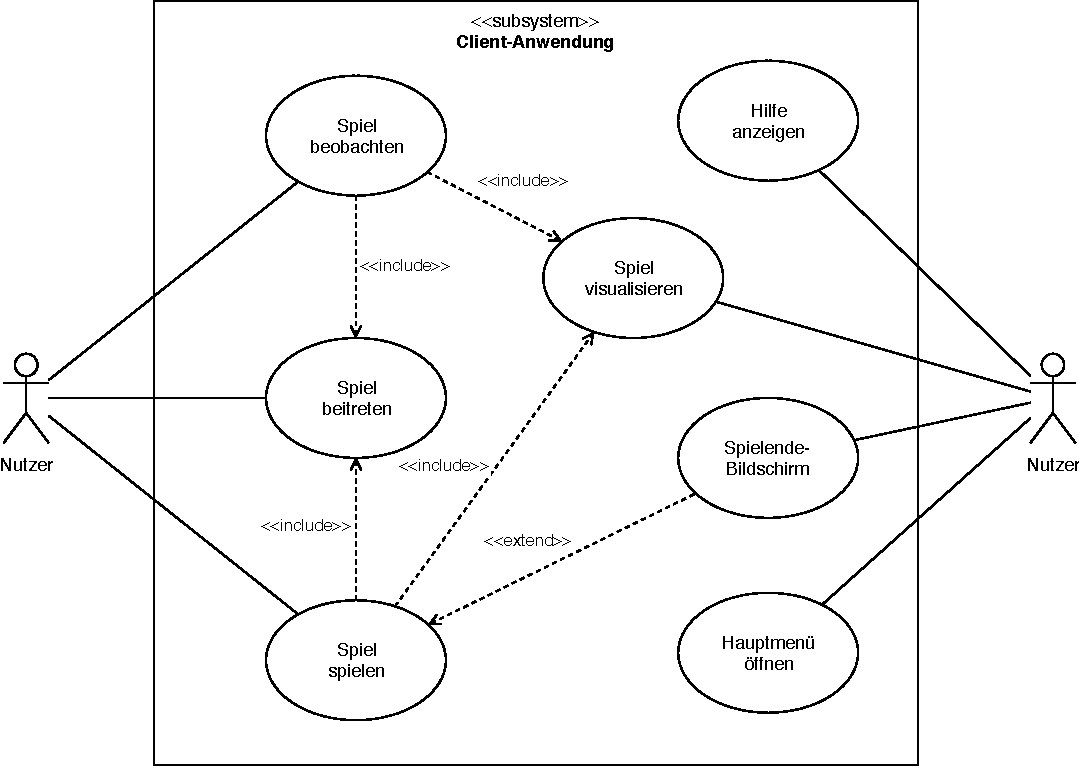
\includepdf[pages=-, scale=0.8, pagecommand={\subsection{Anwendungsfälle}\subsubsection{Client}Anwendungsfälle der Client-Anwendung. Der Anwendungsfall \glqq{}Spiel spielen\grqq{} wird unter \ref{ssec:Partie}~ konkretisiert. Hinweis: Der zweite Akteur wurde nur aus Übersichtlichkeitsgründen hinzugefügt und stellt keinen zweiten Nutzer dar.}]{../Meilenstein02/images/AFD_Client.pdf}

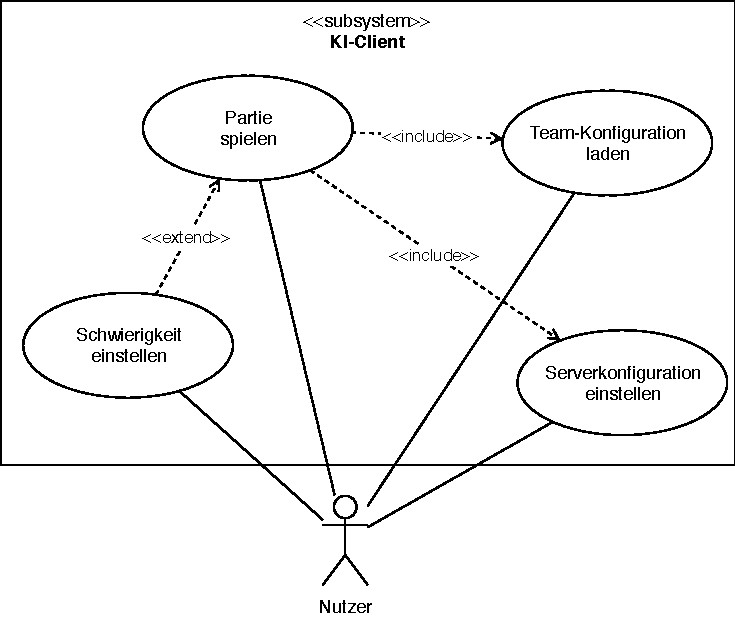
\includepdf[pages=-, scale=0.8, pagecommand={\subsubsection{KI-Client}Anwendungsfälle des KI-Clients. Diese Anwendung verbindet sich mit einem Server und simuliert mithilfe einer zuvor konfigurierten KI einen menschlichen Gegenspieler. Der Anwendungsfall \glqq{}Spiel spielen\grqq{} wird unter \ref{ssec:Partie}~ konkretisiert.}]{../Meilenstein02/images/AFD_KIClient.pdf}

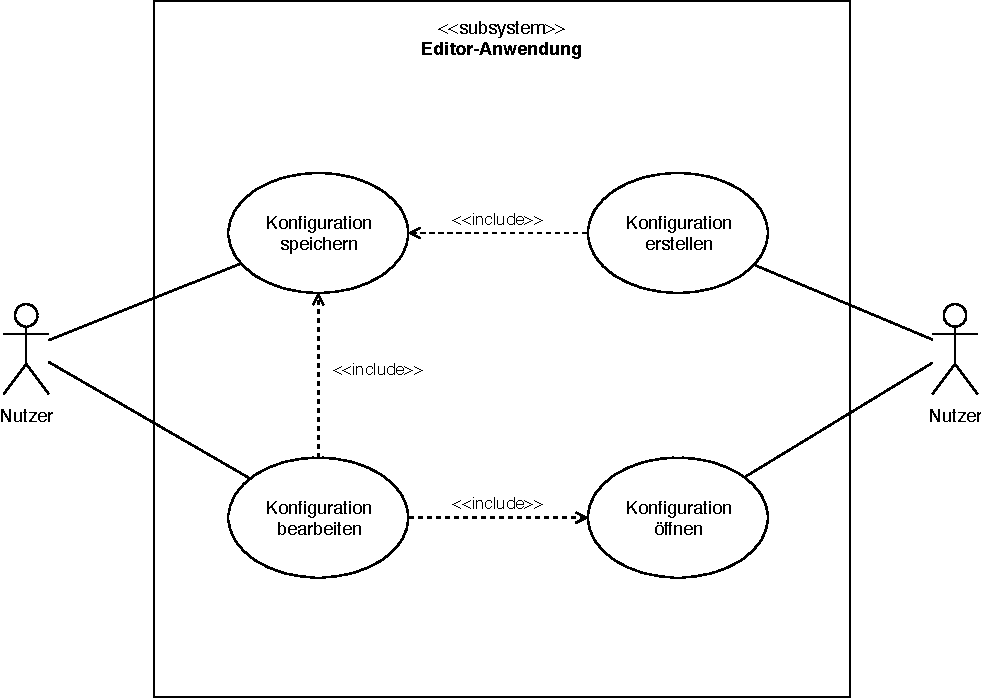
\includepdf[pages=-, scale=0.8, pagecommand={\subsubsection{Editor}Anwendungsfälle der Editor-Anwendung. Der zweite Akteur wurde nur aus Übersichtlichkeitsgründen hinzugefügt und stellt keinen zweiten Nutzer dar.}]{../Meilenstein02/images/AFD_Editor.pdf}
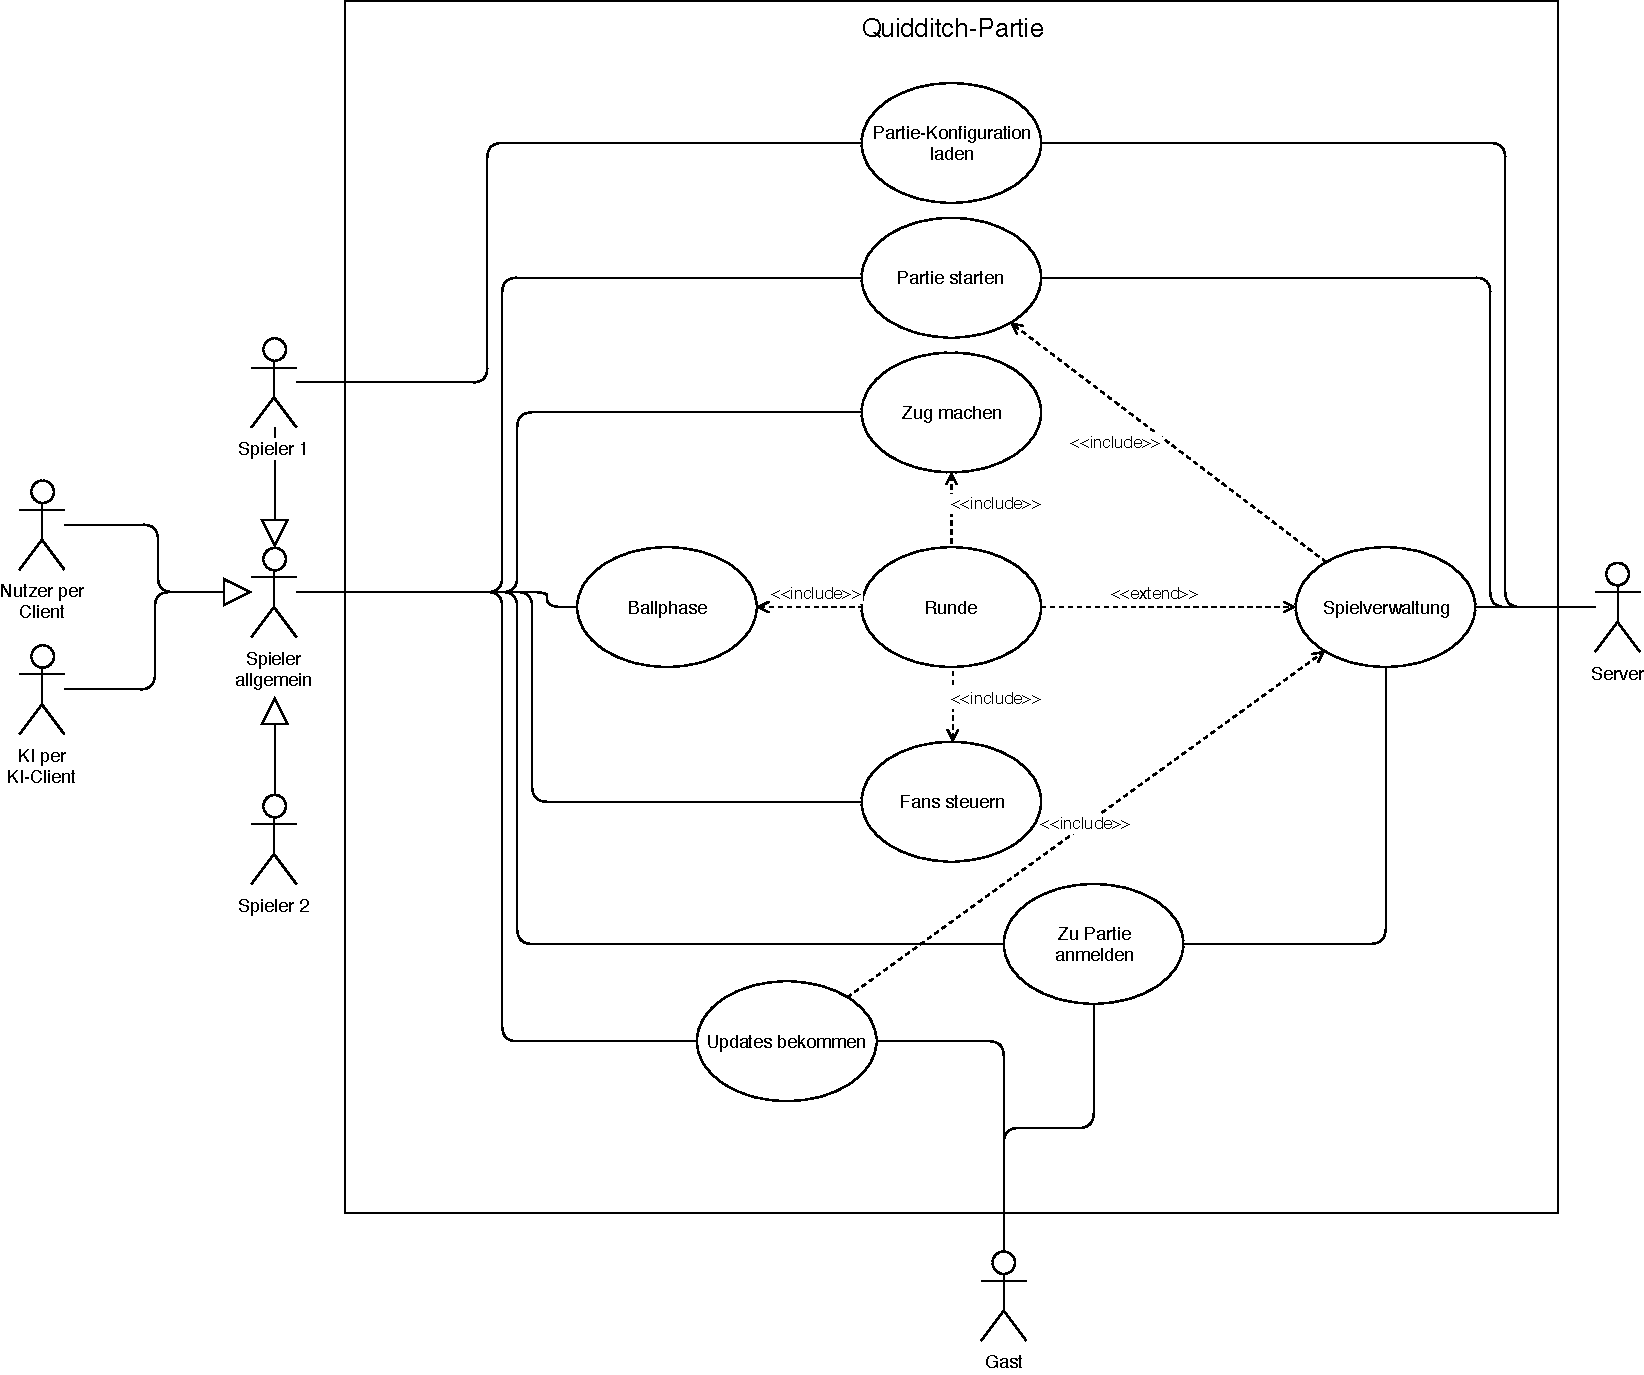
\includepdf[pages=-, scale=0.8, pagecommand={\subsubsection{Partie}\label{ssec:Partie}Mögliche Anwendungsfälle, die während einer Partie auftreten. Die Runde stellt einen abstrakten Anwendungsfall dar, der sich aus den einzelenen Phasen einer Runde zusammensetzt.}]{../Meilenstein02/images/AFD_Party.pdf}


\subsection{Zuordnung der Anforderungen zu Anwendungsfällen}
Hier wird aufgelistet, welche funktionalen Anforderungen (siehe \ref{FAs}) von den jeweiligen Anwendungsfällen abgedeckt werden.
\subsubsection{Hauptmenü öffnen}
FA60

\subsubsection{Hilfe anzeigen}
FA65

\subsubsection{Spielende-Bildschirm}
FA49,
FA62

\subsubsection{Spiel visualisieren}
FA1,
FA2, 
FA3, 
FA4, 
FA5, 
FA6, 
FA64

\subsubsection{Spiel beobachten}
FA55,
FA66

\subsubsection{Spiel beitreten}
FA55,
FA61

\subsubsection{Spiel spielen}
FA14, 
FA15, 
FA16, 
FA17, 
FA18, 
FA19, 
FA20, 
FA55, 
FA67,
FA68, 
FA69,
FA73 

\subsubsection{Serverkonfiguration einstellen}
FA74 

\subsubsection{Team-Konfiguration laden}
FA75 

\subsubsection{Konfiguration erstellen}
FA14,
FA15, 
FA53, 
FA54, 
FA71

\subsubsection{Konfiguration speichern}
FA14,
FA15, 
FA53, 
FA54, 
FA71

\subsubsection{Konfiguration bearbeiten}
FA14,
FA15, 
FA53, 
FA54, 
FA70, 
FA72

\subsubsection{Konfiguration öffnen}
FA14,
FA15, 
FA53, 
FA54, 
FA63

\subsubsection{Team-Konfiguration laden}
FA14,
FA15, 
FA54, 
FA55, 
FA63

\subsubsection{Partie starten}
FA50,
FA51, 
FA55

\subsubsection{Zug machen}
FA8,
FA21, 
FA22, 
FA24, 
FA26, 
FA27, 
FA28, 
FA29, 
FA30, 
FA37, 
FA38, 
FA39, 
FA40, 
FA41, 
FA42, 
FA46, 
FA55

\subsubsection{Runde}
FA10,
FA11, 
FA12, 
FA13, 
FA25, 
FA44, 
FA55

\subsubsection{Ballphase}
FA10,
FA11, 
FA12, 
FA13, 
FA29, 
FA45, 
FA55 

\subsubsection{Fans steuern}
FA31,
FA32, 
FA33, 
FA34, 
FA35, 
FA47, 
FA55 

\subsubsection{Spielverwaltung}
FA1,
FA2, 
FA3, 
FA4, 
FA5, 
FA6, 
FA7, 
FA9, 
FA23, 
FA30, 
FA36, 
FA43, 
FA48, 
FA49, 
FA52, 
FA53, 
FA54, 
FA56, 
FA58, 
FA59 

\subsubsection{Updates bekommen}
FA55

\subsubsection{Zu Partie anmelden}
FA55

\subsubsection{Partie-Konfiguration laden}
FA53,
FA57

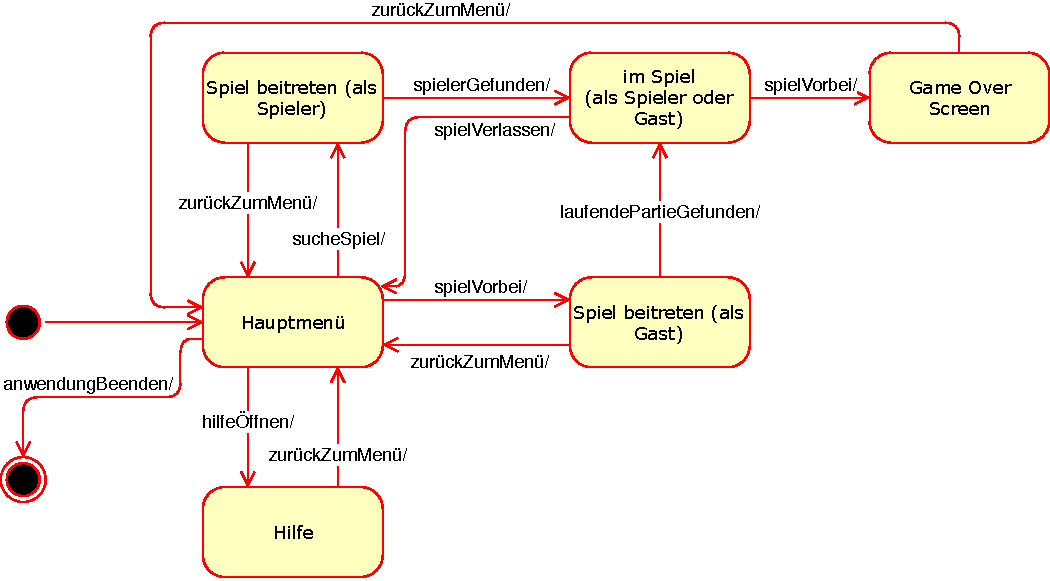
\includepdf[pages=-, scale=0.8, pagecommand={\subsection{Abläufe im System}\subsubsection{State-Machine Clientanwendung} Zustandsdiagramm für die verschiedenen Ansichten der Client-Anwendung.}]{../Meilenstein02/images/Client_SM.pdf}

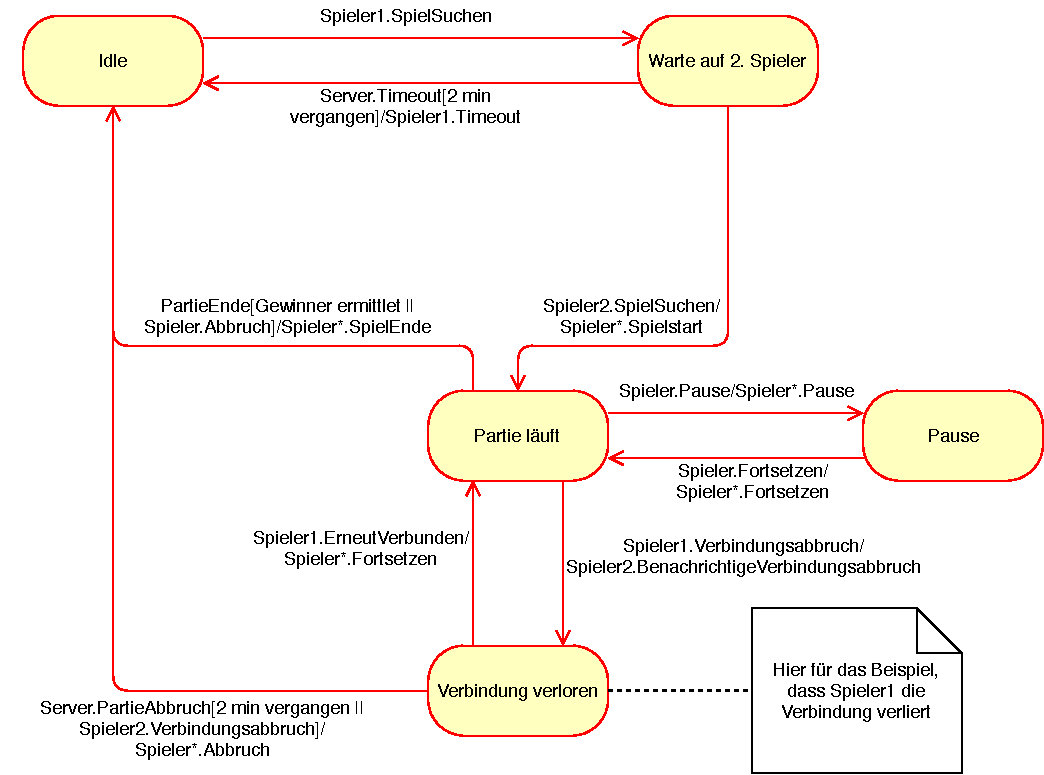
\includepdf[pages=-, scale=0.8, pagecommand={\subsubsection{State-Machine Partie Server} Zustandsdiagramm des Servers für eine komplette Partie, inklusive Anmeldung der Spieler und eventuelle Verbindungsabbrüche.}]{../Meilenstein02/images/SM_Server.pdf}

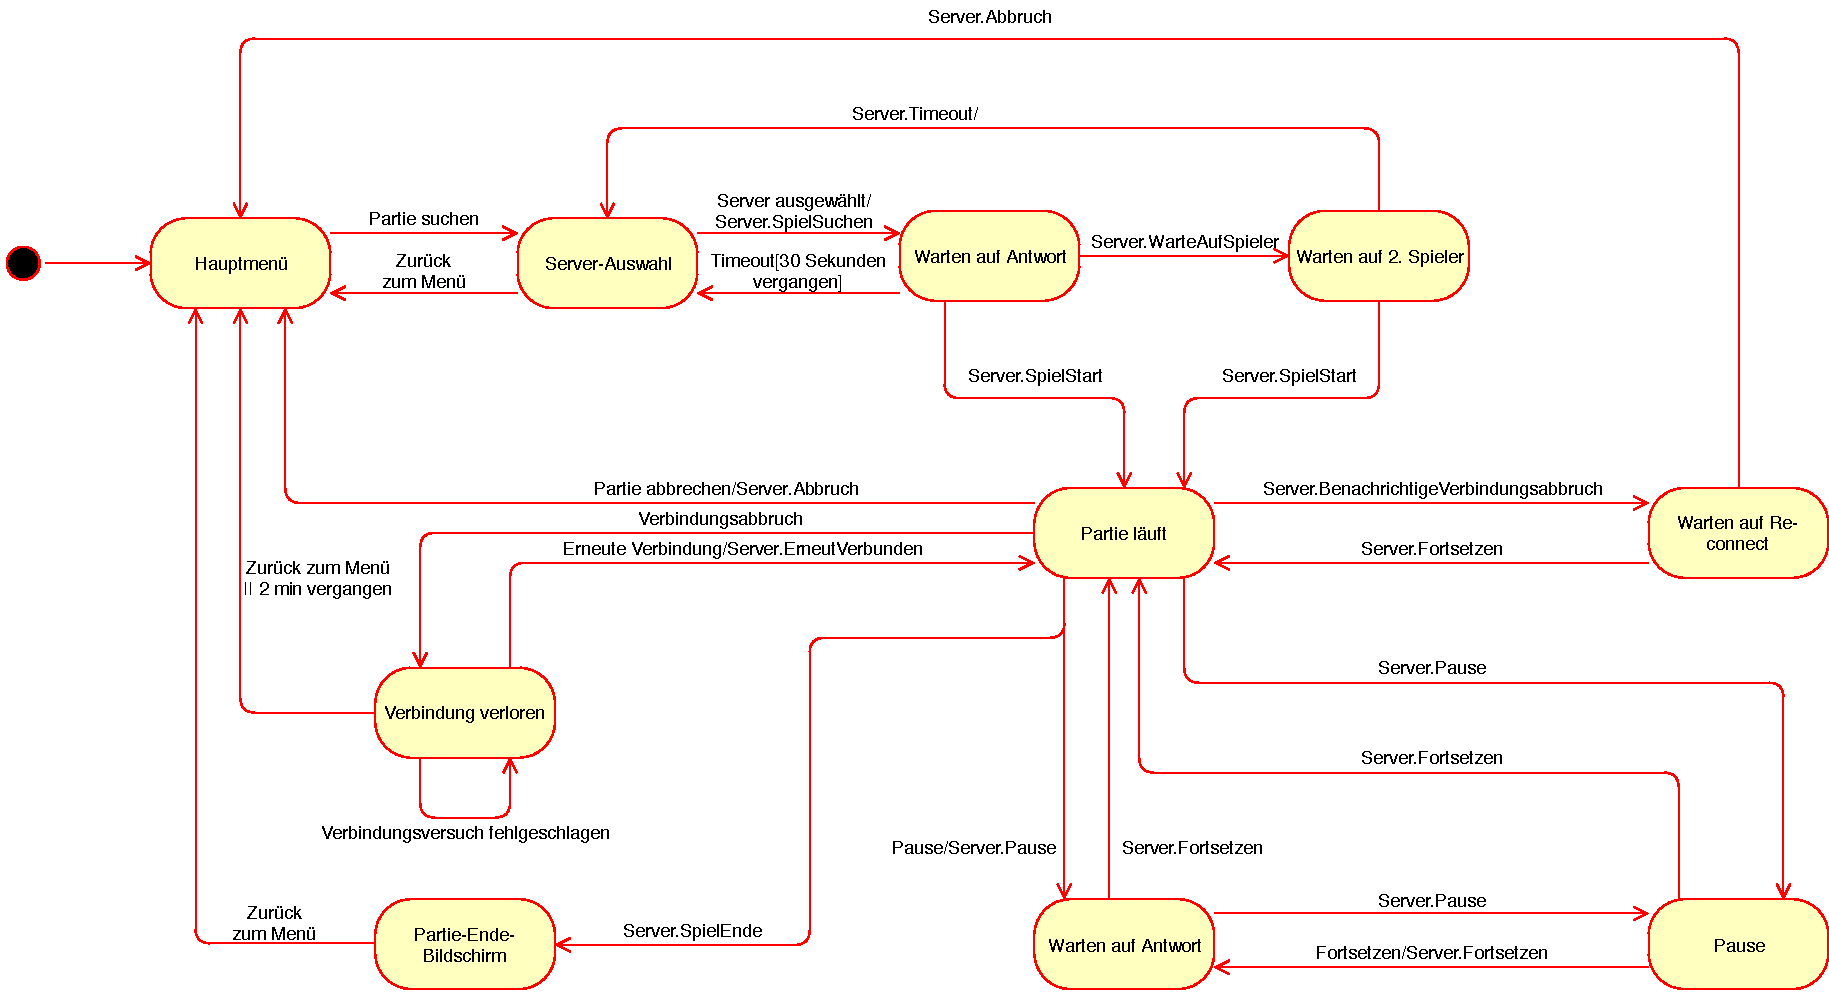
\includepdf[pages=-, scale=0.9, pagecommand={\subsubsection{State-Machine Partie Client}Zustandsdiagramm der Client-Anwendung für eine komplette Partie.}]{../Meilenstein02/images/SM_ClientAnmelden.pdf}

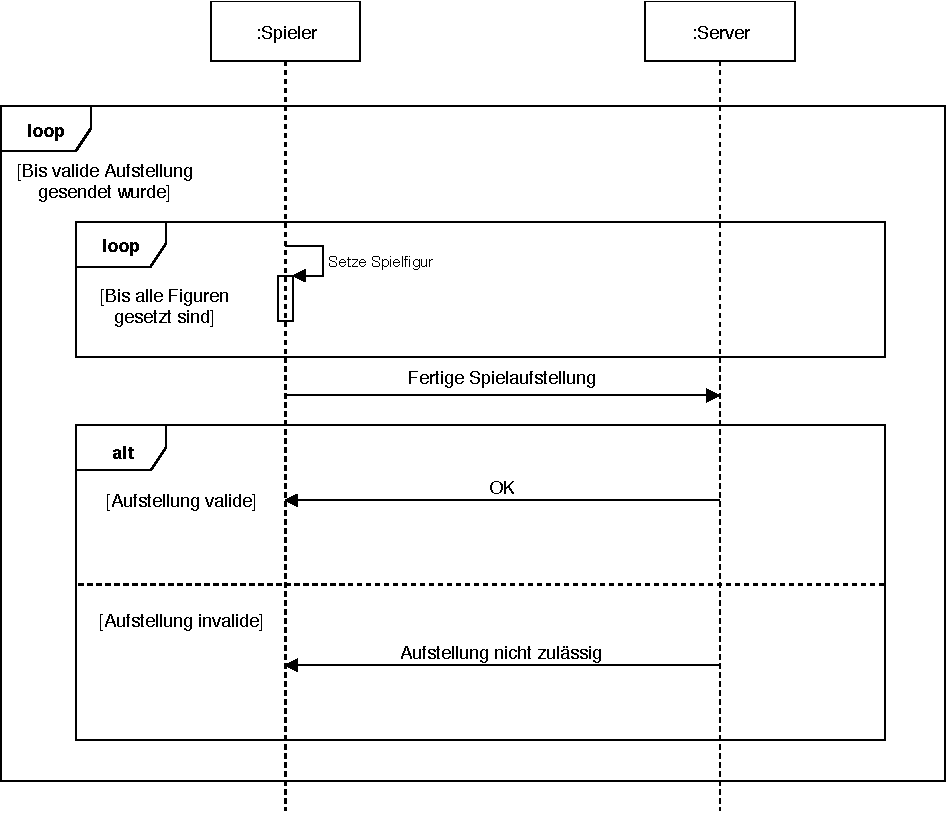
\includepdf[pages=-, scale=0.8, pagecommand={\subsubsection{Sequenzdiagramm Spielaufstellung}Kommunikation zwischen Spieler und Server während der Spielaufstellungsphase.}]{../Meilenstein02/images/SD_Spielaufstellung.pdf}

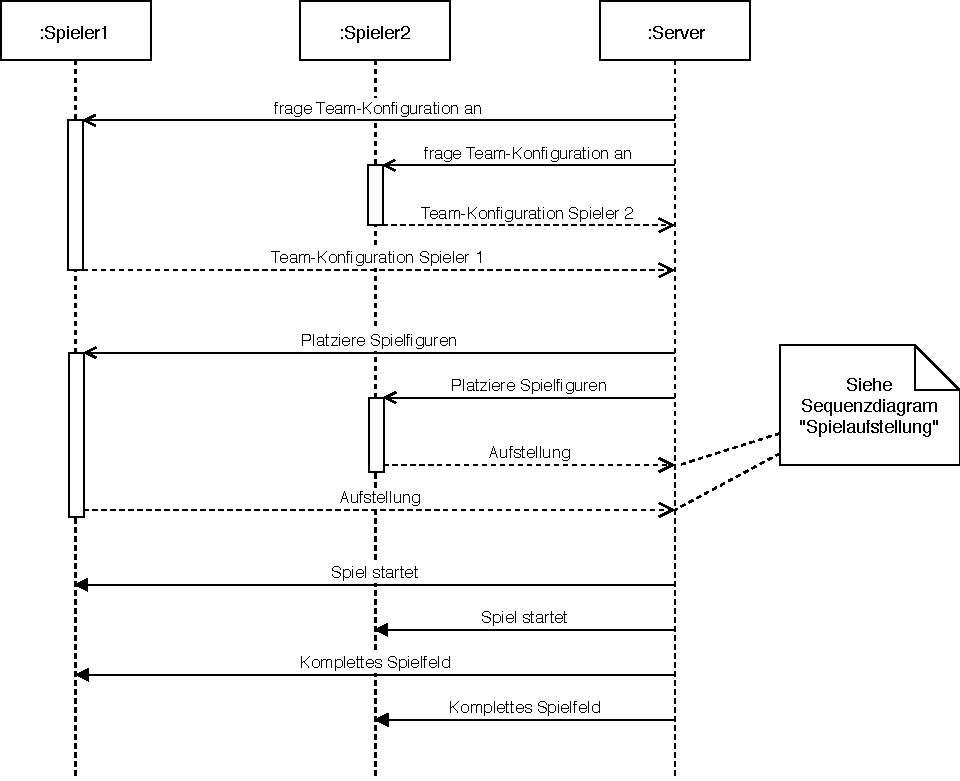
\includepdf[pages=-, scale=0.8, pagecommand={\subsubsection{Sequenzdiagramm Spielvorbereitung}Nachrichtenaustausch zwischen Server und den Spielern während der Vorbereitung auf die Partie.}]{../Meilenstein02/images/SD_Spielvorbereitung.pdf}
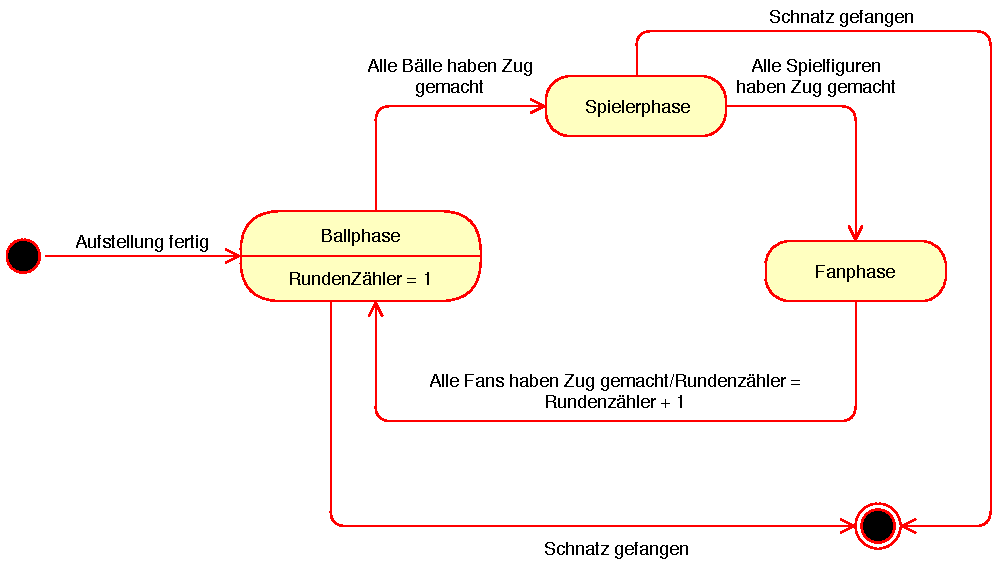
\includepdf[pages=-, scale=0.8, pagecommand={\subsubsection{State-Machine Rundenablauf}Ablauf der Spielphasen im Spiel}]{../Meilenstein02/images/SM_Rundenablauf.pdf}
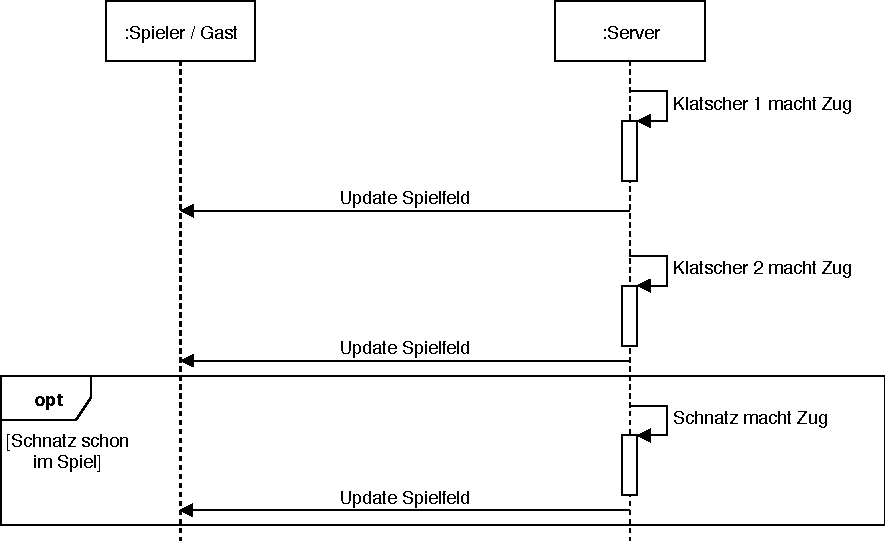
\includepdf[pages=-, scale=0.8, pagecommand={\subsubsection{Sequenzdiagramm Ballphase}}]{../Meilenstein02/images/SD_Ballphase.pdf}
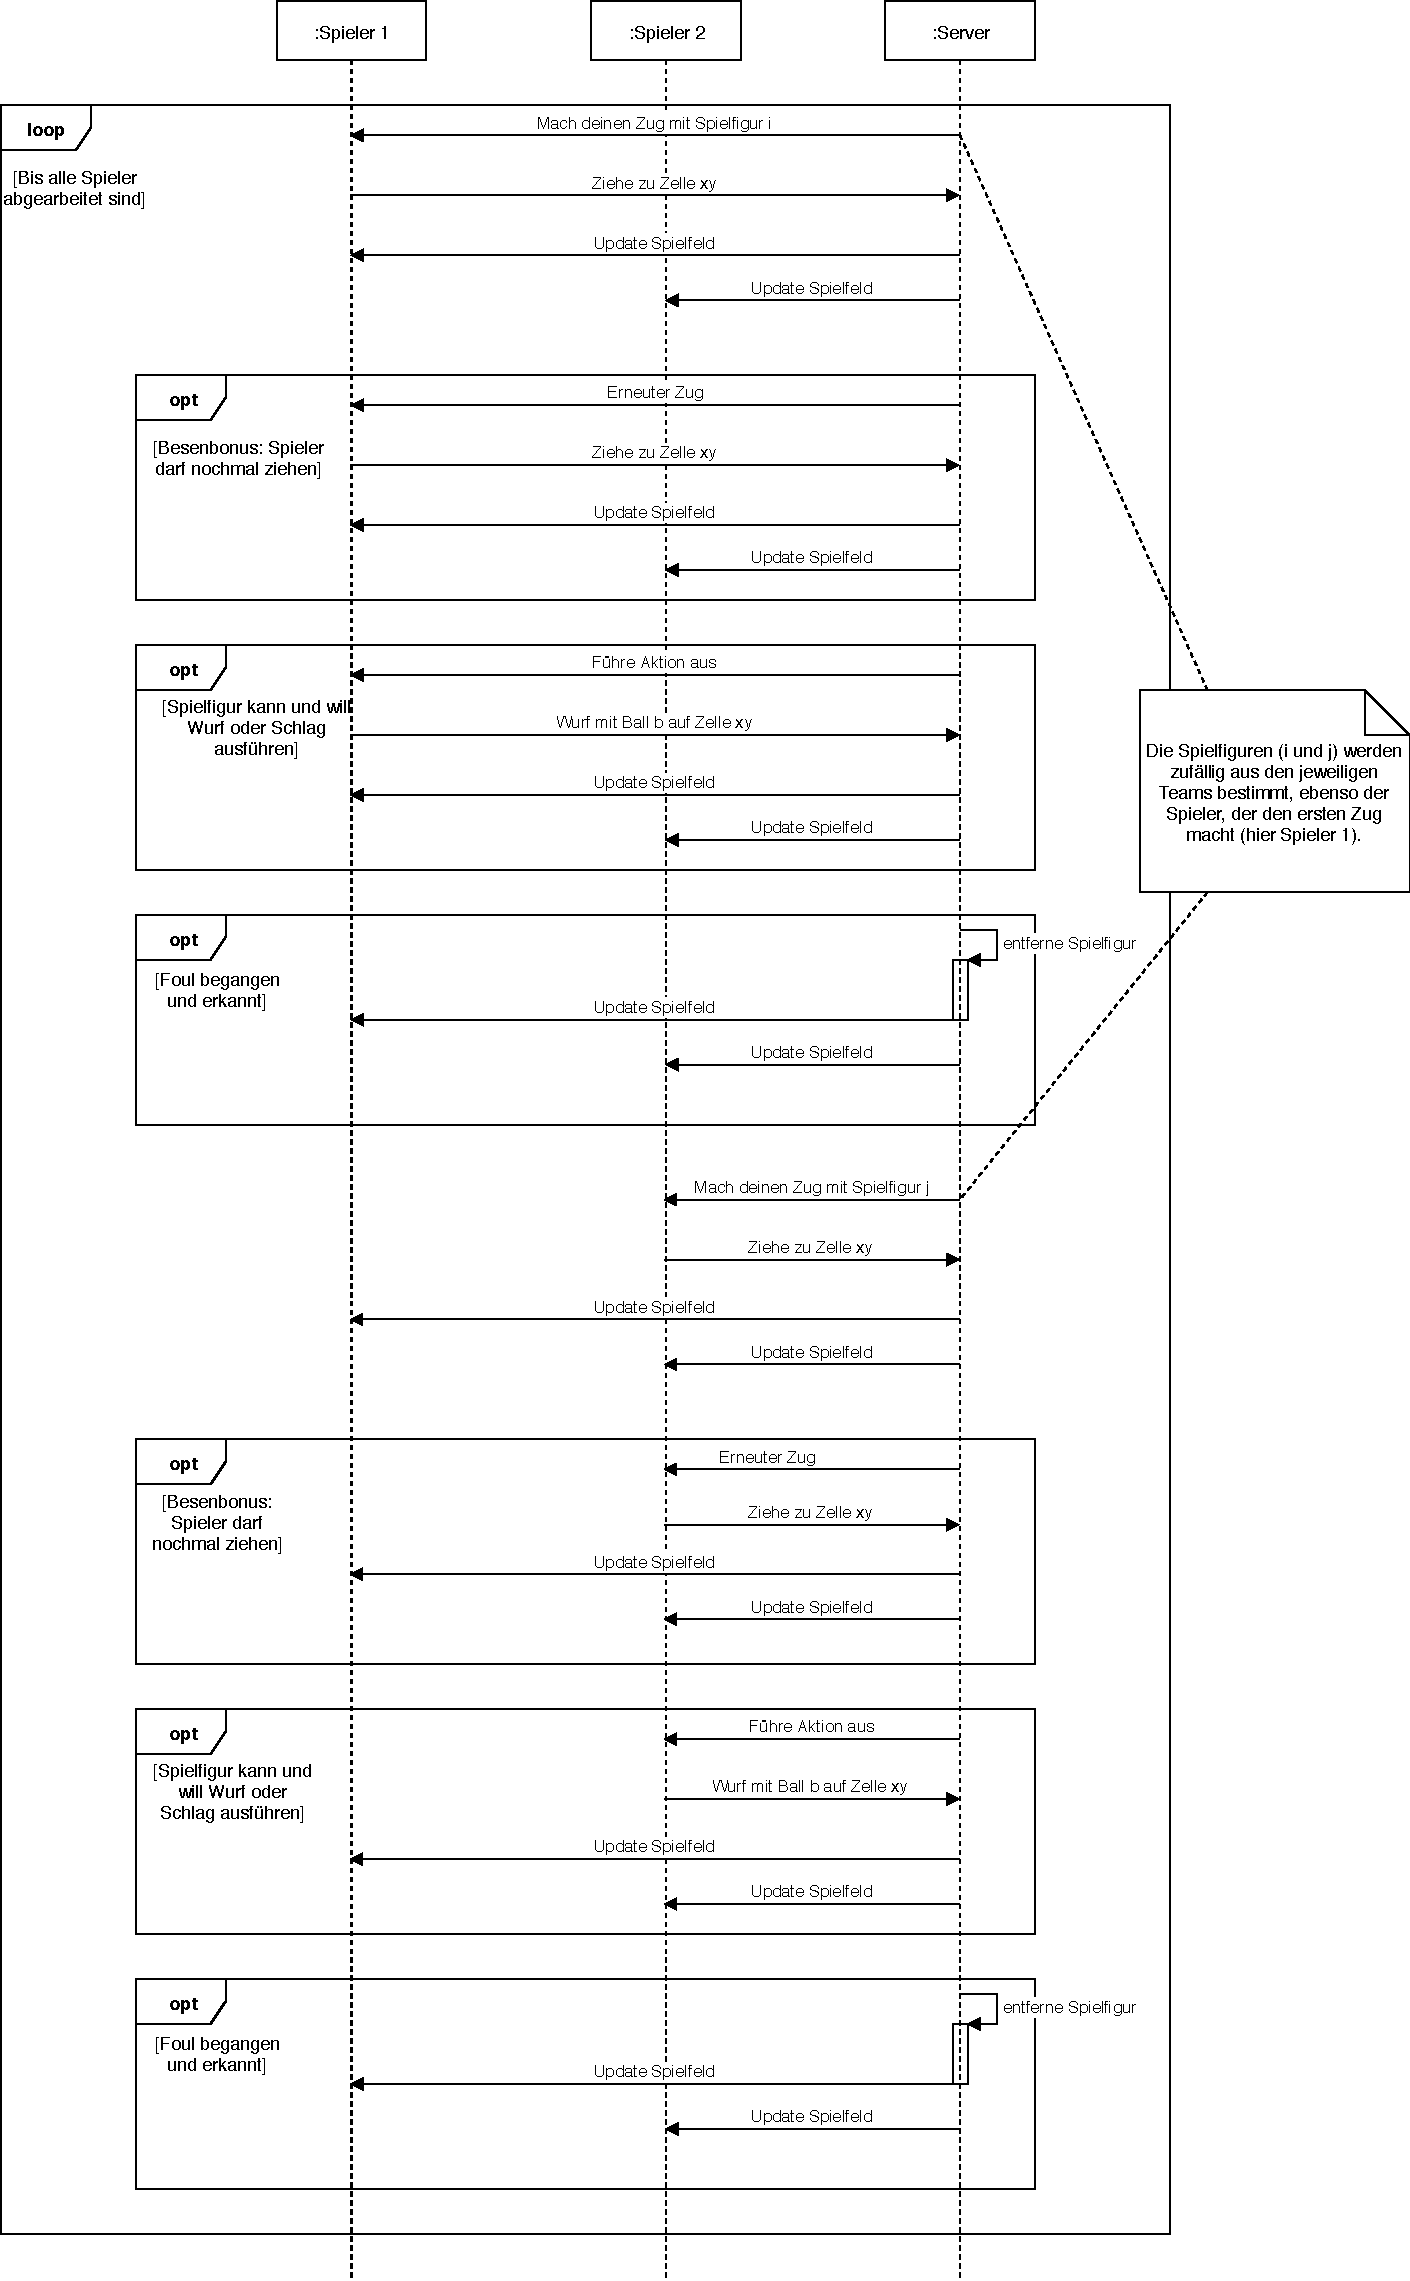
\includepdf[pages=-, scale=0.65, pagecommand={\subsubsection{Sequenzdiagramm Spielerphase}}]{../Meilenstein02/images/SD_Spielerphase.pdf}
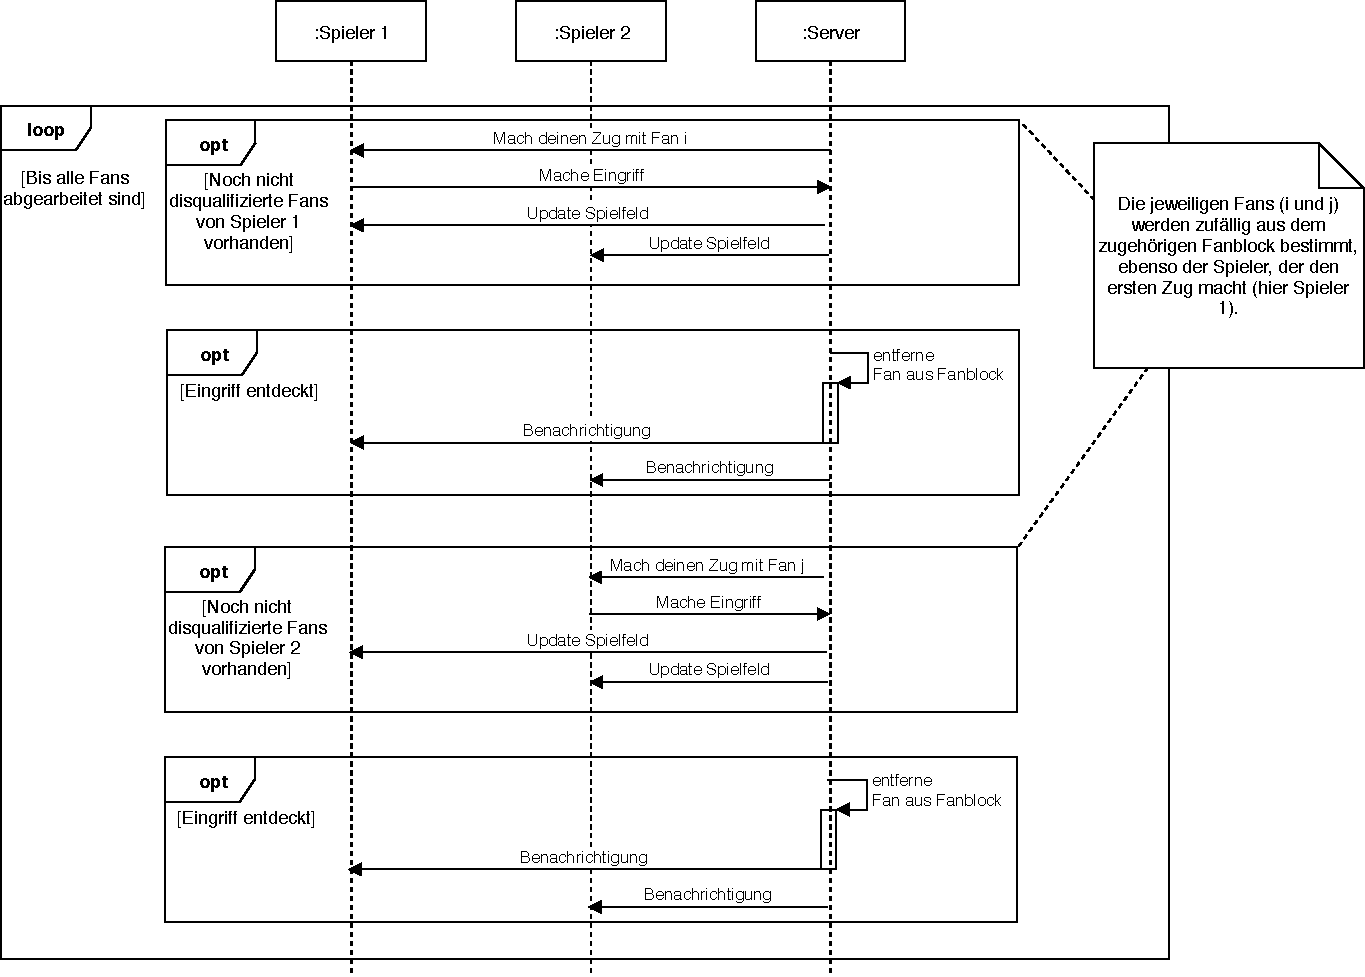
\includepdf[pages=-, scale=0.8, pagecommand={\subsubsection{Sequenzdiagramm Fanphase}}]{../Meilenstein02/images/SD_Fanphase.pdf}
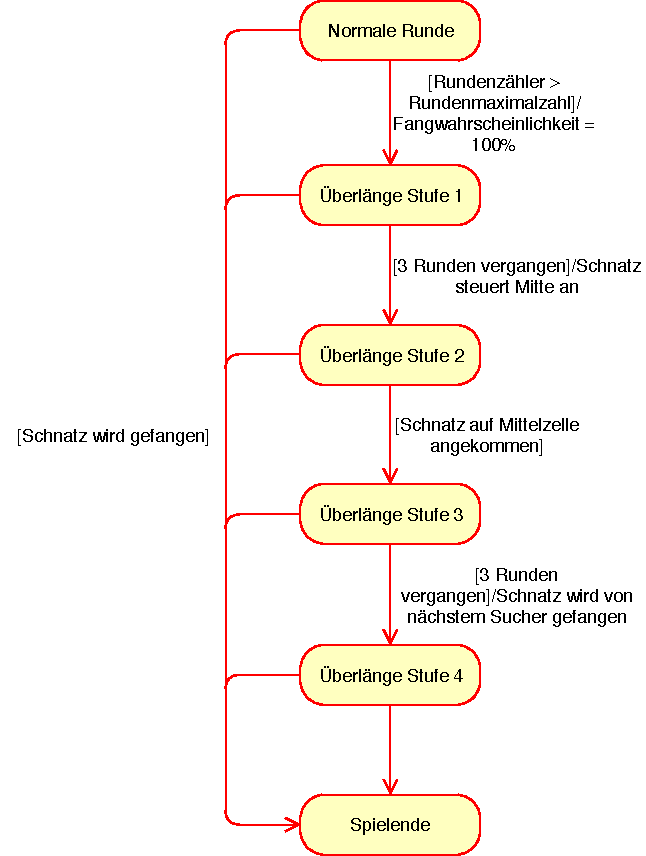
\includepdf[pages=-, scale=0.7, pagecommand={\subsubsection{State-Machine Überlängenbehandlung}}]{../Meilenstein02/images/SM_Ueberlaenge.pdf}
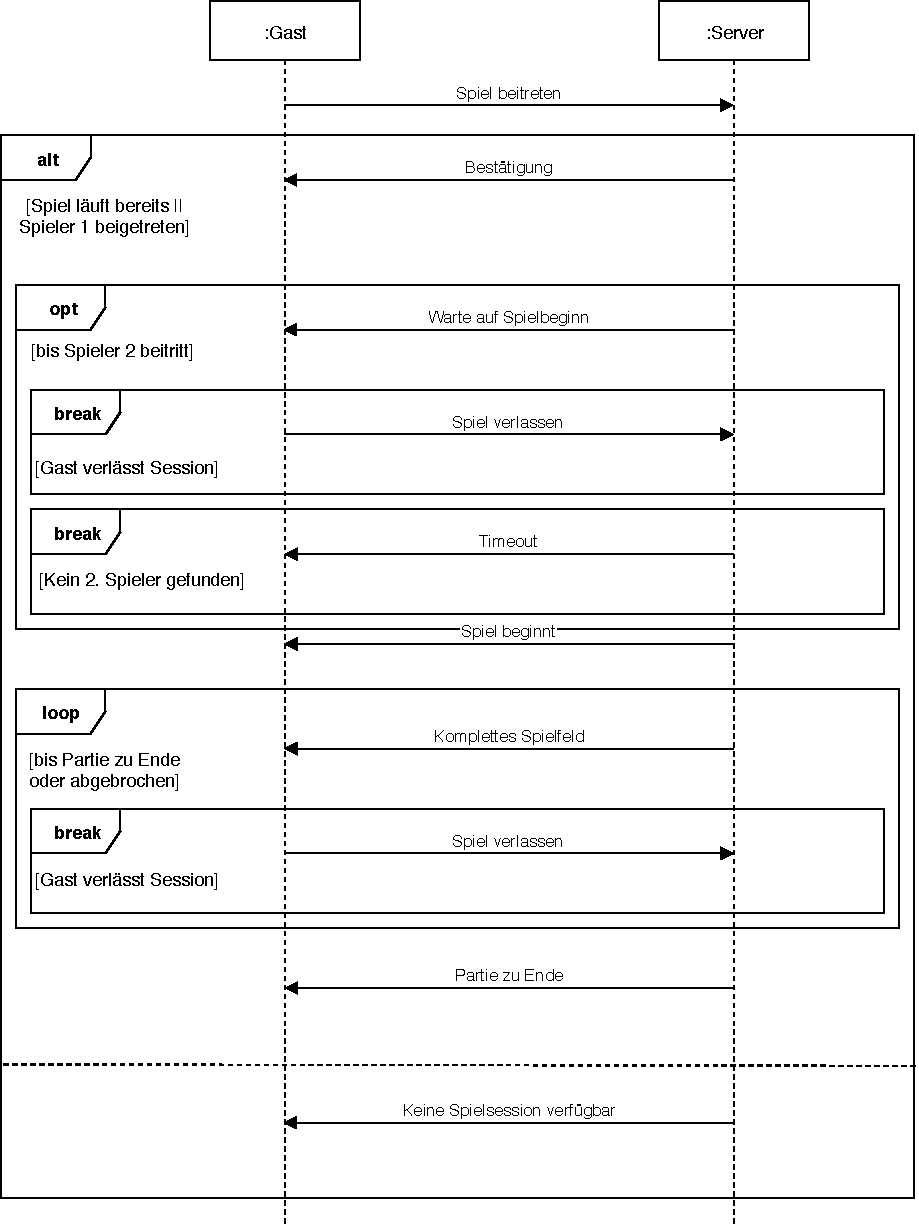
\includepdf[pages=-, scale=0.7, pagecommand={\subsubsection{Sequenzdiagramm Gast}}]{../Meilenstein02/images/SD_Gast.pdf}

    \section{Anforderungsdefinition}
    \textbf{Bemerkungen zu den Abhängigkeiten der Anforderungen:} \\
Abhängigkeiten werden aus Gründen der Übersichtlichkeit vererbt. Beispielsweise besitzt die Zentrumszelle implizit alle Abhängigkeiten des Zentrums.  \\ \\
 \textbf{Bemerkungen zu den Prioritäten:} \\
 \begin{itemize}
    \item[-] Optionale Komponente
    \item[0] Geforderte Komponente
    \item[+] Geforderte, wichtige aber nicht zeitkritisch Komponente
    \item[++] Geforderte, wichtige und zeitkritische Komponente
 \end{itemize}

\subsection{Funktionale Anforderungen: Spielregeln} 

\fanf	{Quidditch-Spielfeld}
        {Das Quidditch-Spielfeld hat eine Ovale Form, die in ein Raster von 17x13 quadratischen Zellen eingepasst ist. Auf diesem Feld finden alle Spielhandlungen statt, die während dem Spiel getätigt werden können.}
        {Das Spielfeld ist die zentrale Komponente des Spiels, da sich hier während einer Partie sämtliche Abläufe abspielen.}
        {-}
        {++}
        {Spieler, KI, Gast, Client, KI-Client, Server}

\fanf	{Zentrum}
        {Das Zentrum ist ein Bereich auf dem Quidditch-Spielfeld, der in der Mitte angeordnet ist und aus 3x3 quadratischen Zellen besteht. Zu Beginn dürfen sich hier keine Spielfiguren befinden.}
        {Das Zentrum markiert den Bereich um die Zentrumszelle des Spielfeldes, in dem das Spiel gestartet wird.}
        {Spielfeld}
        {+}
        {Spieler, KI, Gast, Client, KI-Client, Server}

\fanf	{Zentrumszelle}
        {Die Zentrumszelle stellt den mittleren Punkt des Zentrums dar.}
        {Die Zentrumszelle ist der Startpunkt für die Bälle beim Spielstart.}
        {Zentrum}
        {+}
        {Spieler, KI, Gast, Client, KI-Client, Server}

\fanf	{Hüterzonen}
        {Die Hüterzonen sind an den jeweils gegenüberliegenden Seiten des Quidditch-Spielfeldes platziert. Die Hüterzonen sind oval förmig, bestehen aus $11x5$ Zellen und beinhalten jeweils drei Torringe.}
        {In den Hüterzonen können die Teams Punkte erzielen.}
        {Spielfeld}
        {++}
        {Spieler, KI, Gast, Client, KI-Client, Server}
        
\fanf	{Zelle}
        {Die Zelle ist die kleinste Einheit des Spielfeldes, auf ihr darf sich immer nur eine Spielfigur gleichzeitig befinden. Bälle können sich jedoch eine Zelle mit einem anderen Ball und / oder einer Spielfigur teilen.}
        {Das gesamte Spielfeld ist aus Zellen aufgebaut. Sie bestimmen, wie sich Spielobjekte bewegen können.}
        {Spielfeld}
        {++}
        {Spieler, KI, Gast, Client, KI-Client, Server}

\fanf	{Torring}
        {Die Teams können Punkte erzielen, indem sie den Quaffel durch einen gegnerischen Torring werfen.}
        {Die Torringe dienen den Teams als Hauptquelle von Punkten.}
        {Hüterzone}
        {++}
        {Spieler, KI, Gast, Client, KI-Client, Server}
        
\fanf	{Schussvektorberechnung}
        {Ein Schussvektor zeigt vom Mittelpunkt der Startzelle auf die Zielzelle des Wurfs. Alle Zellen, die von diesem Vektor geschnitten werden, sind so genannte überstrichene Zellen.}
        {Ein Schussvektor beschreibt, wie eine Spielfigur einen Ball über das Spielfeld bewegten kann.}
        {Zelle}
        {++}
        {Spieler, KI, Gast, Client, KI-Client, Server}
        
\fanf	{Punkte erzielen}
        {Es gibt zwei Möglichkeiten, Punkte zu erzielen: Den Quaffel durch ein gegnerischen Torring werfen (entspricht 10 Punkten) oder den Goldenen Schnatz fangen (entspricht 30 Punkten).}
        {Die Punktezahl zeigt an, welcher Spieler sich im Moment besser schlägt und dient zur Bestimmung des Gewinners am Ende der Partie.}
        {Schnatz fangen, Quaffel werfen}
        {+}
        {Spieler, KI, Gast, Client, KI-Client, Server}

\fanf	{Entfernungsberechnung}
        {Die Entfernung zwischen zwei Zellen ist die kleinstmögliche Anzahl an Zügen, die man braucht, um von Zelle A zu Zelle B zu kommen. Dabei darf  man sich in alle Richtungen bewegen, also vertikal, horizontal und Diagonal.}
        {Die Entfernung ist maßgeblich für den Erfolg von verschiedenen Aktionen, wie z.B. dem Werfen des Quaffels.}
        {Zelle}
        {++}
        {Spieler, KI, Gast, Client, KI-Client, Server}

\fanf	{Bälle}
        {Es gibt 3 verschiedene Arten von Bällen: Den Quaffel, die Klatscher und den Schnatz.}
        {Die Bälle sind zentraler Bestandteil des Spiels.}
        {-}
        {++}
        {Spieler, KI, Gast, Client, KI-Client, Server}

\fanf	{Quaffel [Ball]}
        {Der Quaffel ist ein roter Lederball, mit dem die Team Punkte erzielen kann.}
        {Der Quaffel ist die zentrale Punktequelle.}
        {Bälle}
        {++}
        {Spieler, KI, Gast, Client, KI-Client, Server}

\fanf	{Klatscher [Ball]}
        {Die Klatscher sind kleine schwarze Bälle, die sich von alleine auf Spieler zubewegen (eine Zelle pro Runde), die keine Treiber sind.}
        {Die Klatscher verleihen dem Spiel zusätzliche taktische Tiefe, da sie Spielfiguren für eine Runde ausschalten können.}
        {Bälle}
        {++}
        {Spieler, KI, Gast, Client, KI-Client, Server}

\fanf	{Schnatz [Ball]}
        {Der Schnatz ist eine kleiner goldener Ball, sich von alleine von Suchern wegbewegt (eine Zelle pro Runde). Das bedeutet, er achtet auf den nächsten Sucher, und wählt unter allen möglichen freien Zellen, die eine größere Entfernung zu diesem haben, als seine gegenwärtige, eine zufällige aus, und bewegt sich auf diese Zelle. Falls es keine solchen Zellen gibt, bewegt sich der Schnatz auf eine zufällige freie Nachbarzelle. Der Schnatz erscheint zu Beginn der dreizehnten Runde auf einer zufällig gewählten freien Zelle, die möglichst gleich weit von beiden Suchern entfernt ist.}
        {Der Schnatz dient zum Punkteerzielen und führt, wenn er gefangen wird, zum Ende des Partie.}
        {Bälle}
        {++}
        {Spieler, KI, Gast, Client, KI-Client, Server}

\fanf	{Besen}
        {Jede Spielfigur besitzt einen Besen, die einen der folgenden Typen haben: Zauberfauch, Sauberwisch 11, Komet 2-60, Nimbus 2001 oder Feuerblitz. Der Typ des Besens bestimmt die Wahrscheinlichkeit, mit der eine Spielfigur nach einer Bewegung um eine Zelle eine weitere Bewegung ausführen darf. Diese Wahrscheinlichkeit wird in der Partiekonfiguration festgelegt, wobei die Besen in der genannten Reihenfolge aufsteigende Wahrscheinlichkeiten besitzen.}
        {Die Besen geben den Spielfiguren eine unterschiedliche Qualität.}
        {-}
        {+}
        {Spieler, KI, Gast, Client, KI-Client, Server}
        
\fanf	{Teams}
        {Ein Team besteht aus sieben Spielfiguren und sieben Einmischungen. Außerdem hat jedes Team einen Namen, ein Motto, eine Hauptteamfarbe und eine Ersatzteamfarbe. Die sieben Spielfiguren Teilen sich wie folgt auf:  ein Hüter, zwei Treiber, drei Jäger und ein Sucher. Bei den Spielfiguren darf jedes Geschlecht bis zu vier mal vertreten sein. Zudem muss jeder Besentyp einmal vertreten sein. Bei den sieben Fans muss jeder Fantyp mindestens einmal vertreten sein.}
        {Quidditch ist ein Teamspiel, weshalb Teams benötigt werden.}
        {Spielfigur, Fans, Besen}
        {+}
        {Spieler, KI, Gast, Client, KI-Client, Server}

\fanf	{Spielfiguren}
        {Es gibt 4 Arten von Spielfiguren: Jäger, Sucher, Hüter und Treiber. Jede Spielfigur hat dabei einen Namen und ein Geschlecht.}
        {Die unterschiedlichen Typen der Spielfiguren geben dem Spiel taktische Tiefe.}
        {-}
        {++}
        {Spieler, KI, Gast, Client, KI-Client, Server}

\fanf	{Jäger [Spielfigur]}
        {Jäger können den Quaffel aufnehmen und werfen und damit Punkte für ihr Team erzielen.}
        {Jäger können Punkte für ihr Team erzielen.}
        {Spielfigur}
        {++}
        {Spieler, KI, Gast, Client, KI-Client, Server}

\fanf	{Treiber [Spielfigur]}
        {Treiber können den Klatscher schlagen und somit zum Gegner hin und / oder von Teammitgliedern weg befördern.}
        {Treiber dienen zum Schutz des eigenen Teams vor den Klatschern. Gleichzeitig können sie den Gegner aktiv sabotieren, in dem sie ihm den Klatscher zuspielen.}
        {Spielfigur}
        {++}
        {Spieler, KI, Gast, Client, KI-Client, Server}

\fanf	{Hüter [Spielfigur]}
        {Hüter können den Quaffel aufnehmen und versuchen, den Gegner daran zu hindern, ein Tor zu erzielen. Landet der Quaffel auf einem Torring so geht der Quaffel am ende der Rudenphase in den Besitz des Hüters über, wenn er sich selbst in der Hüterzone befindet. Ein Hüter kann selbst keine Tore erzielen.}
        {Hüter stellen die Verteidigung seines Teams dar.}
        {Spielfigur, Hüterzone}
        {++}
        {Spieler, KI, Gast, Client, KI-Client, Server}

\fanf	{Sucher [Spielfigur]}
        {Sucher versuchen den Schnatz zu finden, um Punkte zu erzielen und das Spiel zu beenden.}
        {Der Sucher beendet das Spiel.}
        {Spielfigur}
        {++}
        {Spieler, KI, Gast, Client, KI-Client, Server}
        
\fanf	{Quaffel Schießen}
        {Hüter und Jäger können den Quaffel schießen. Der Wurf wird über ein Schussvektor angegeben. Jede gegnerische Spielfigur, die sich auf einer überstrichenen Zelle des Schussvektors befindet, kann den Quaffel abfangen. Wird der Ball von keiner Spielfigur abgefangen, so ist der Wurf mit der Wahrscheinlichkeit $P^d$ erfolgreich, wobei $P$ eine elementare Wurfwahrscheinlichkeit und $d$ die Entfernung zur Zielzelle ist. War der Schuss erfolgreich, so landet der Quaffel auf der Zielzelle. Wenn nicht wird der Quaffel auf einer zufälligen freien Zelle in einem $n\times n$ Quadrat um die Zielzelle platziert, wobei $n=\ceil{ \frac{d}{7}}$ ist.}			
        {Das Werfen des Quaffels ermöglicht Passspiel und das erzielen von Punkten.}
        {Schussvektorberechnung, Entfernungsberechnung, Jäger, Hüter, Quaffel}
        {++}
        {Spieler, KI, Gast, Client, KI-Client, Server}
        
\fanf	{Quaffel Abfangen}
        {Jede gegnerische Spielfigur auf einer überstrichenen Zelle des Schussvektors eines Wurfes hat eine gewisse Wahrscheinlichkeit, den Quaffel abzufangen. Diese Wahrscheinlichkeit ist in der Partiekonfiguration vermerkt. Gelingt das Abfangen, so landet der Quaffel auf der Zelle der Abfangenden Spielfigur.}
        {Das Abfangen bietet die Möglichkeit, Würfe des Gegners zu unterbinden.}
        {Quaffel-Werfen, Spielfiguren }
        {++}
        {Spieler, KI, Gast, Client, KI-Client, Server}
        
\fanf	{Quaffel Abprallen}
        {Landet der Quaffel auf einer Zelle, auf der sich eine Spielfigur befindet, die weder Hüter noch Jäger ist, so wird der Quaffel auf eine zufällige freie Nachbarzelle gesetzt.}
        {Nur Jäger und Hüter können direkt mit der Quaffel interagieren.}
        {Sucher, Treiber, Quaffel}
        {+}
        {Spieler, KI, Gast, Client, KI-Client, Server}		
        
\fanf	{Quaffel Halten}
        {Ein Jäger oder Hüter kann den Quaffel halten, wodurch sich der Quaffel immer auf der selben Zelle befindet wie besagter Jäger bzw. Hüter.}
        {Jäger und Hüter sollen den Quaffel, ohne zu passen, über das Spielfeld transportieren können.}
        {Jäger, Hüter, Quaffel}
        {+}
        {Spieler, KI, Gast, Client, KI-Client, Server}	
        
\fanf	{Quaffel Verlieren}
        {Ein Jäger kann den Quaffel verlieren, dass bedeutet, das der Quaffel auf ein freie Nachbarzelle zufällig bewegt wird.}
        {Durch das Verlieren des Quaffels werden Tore im Alleingang erschwert.}
        {Jäger, Hüter, Quaffel, Fouls, Klatscher}
        {+}
        {Spieler, KI, Gast, Client, KI-Client, Server}
    
\fanf	{Quaffel Übernehmen}
        {Ein Jäger darf von einem anderen Jäger den Quaffel übernehmen, sofern dieser auf einem seiner Nachbarzellen ist. Dies gelingt allerdings nur mit einer bestimmten Wahrscheinlichkeit. Jäger dürfen auch von einem gegnerischen Hüter den Quaffel übernehmen, jedoch dies geht nur, wenn sich der Hüter nicht in seiner eigenen Hüterzone befindet.}
        {Bietet zusätzliche Möglichkeiten, den Ball zu erobern.}
        {Jäger, Hüter, Quaffel}
        {+}
        {Spieler, KI, Gast, Client, KI-Client, Server}

\fanf	{Tor Erzielen}
        {Ein Jäger kann ein Tor erzielen, indem er den Quaffel erfolgreich auf eine Torringzelle wirft. Dabei muss der Schussvektor des Wurfes durch die linke oder rechte Seite der Torringzelle gehen.}
        {Stellt für einen Jäger die Möglichkeit dar, Punkte zu erzielen.}
        {Torring, Quaffel Werfen, Jäger}
        {+}
        {Spieler, KI, Gast, Client, KI-Client, Server}
        
\fanf	{Klatscher Schlagen}
        {Ein Treiber kann einen Klatscher schlagen, wenn er sich auf derselben Zelle wie der Klatscher befindet. Der Treiber wählt, um den Klatscher zu schlagen, eine Zielzelle aus, die eine maximale Entfernung von drei zu ihm hat. Zusätzlich müssen auch alle überstrichenen Zellen frei sein. Ist dies beides der Fall, so wird das Schlagen des Klatschers wie ein normaler Quaffel-Wurf behandelt, allerdings mit einer Wahrscheinlichkeit von $100\%$.}
        {Stellt für den Treiber die Möglichkeit dar, den Katscher zu bewegen.}
        {Spielfeld, Treiber, Klatscher}
        {+}
        {Spieler, KI, Gast, Client, KI-Client, Server}
        
\fanf	{Spieler Betäuben}
        {Bewegt sich der Klatscher auf deine Zelle, auf der sich eine Spielfigur befindet, die kein Treiber ist, wird diese mit einer gewissen Wahrscheinlichkeit betäubt. Das hat zur Folge, dass diese Spielfigur gegebenenfalls den Quaffel verliert, keinen Ball fangen und für eine Runde keine Aktion ausführen kann. Der Klatscher, der den Spieler betäubt hat, wird auf eine zufällige freie Zelle gesetzt.}
        {Stellt ein zusätzliches taktisches Spielelement dar.}
        {Klatscher, Jäger, Hüter, Sucher}
        {+}
        {Spieler, KI, Gast, Client, KI-Client, Server}
        
\fanf	{Schnatz Fangen}
        {Befinden sich ein Sucher und der Schnatz auf derselben Zelle, so fängt der Sucher den Schnatz mit einer gewissen Wahrscheinlichkeit. Dadurch erhält sein Team 30 Punkte und das Spiel ist zu Ende.}
        {Das Schnatz Fange führ das Ende der Partie herbei.}
        {Schnatz, Sucher, Punkte}
        {++}
        {Spieler, KI, Gast, Client, KI-Client, Server}
        

\fanf	{Einmischung}
        {Eine  Einmischung ist eine Aktion, die das eigene Team unterstützt und / oder das gegnerische Team schwächt. Diese Einmischungen werden mit einer gewissen Wahrscheinlichkeit durchgeführt und wird vom jeweiligen Spieler in der Endphase ausgelöst. Es gibt die folgenden Typen von Einmischungen: Teleportation, Fernangiff, Impus und Schnatzstoß.}
        {Sorgen für Abwechslung, Witz, und Überraschungen im Spiel.}
        {-}
        {0}
        {Spieler, KI, Gast, Client, KI-Client, Server}

\fanf	{Teleportation [Einmischungstyp]}
        {Bei der Teleportation wird ein Spieler von der eigenen oder auch von der gegnerischen Mannschaft auf eine zufällige freie Zelle teleportiert.}
        {Siehe Einmischung}
        {Einmischung}
        {0}
        {Spieler, KI, Gast, Client, KI-Client, Server}

\fanf	{Fernangriff [Einmischungstyp]}
        {Der Fernangriff bewirkt, dass der getroffene Spieler den Quaffel verliert, sofern er diesen hat und anschließend auf eine zufällige freie Nachbarzelle gestoßen wird.}
        {Siehe Einmischung}
        {Einmischung}
        {0}
        {Spieler, KI, Gast, Client, KI-Client, Server}

\fanf	{Impuls [Einmischungstyp]}
        {Der Impuls sorgt dafür, dass ein Spieler den Quaffel verliert.}
        {Siehe Einmischung}
        {Einmischung}
        {0}
        {Spieler, KI, Gast, Client, KI-Client, Server}

\fanf	{Schnatzstoß [Einmischungstyp]}
        {Bei einem Schnatzstoß macht der Schnatz eine Ausweichbewegung auf eine freie Nachbarzelle.}
        {Siehe Einmischung}
        {Einmischung}
        {0}
        {Spieler, KI, Gast, Client, KI-Client, Server}
        
\fanf	{Schiedsrichter}
        {Der Schiedsrichter ahndet mit einer gewissen Wahrscheinlichkeit Fouls von Spielern oder Einmischungen. Ahndet der Schiedsrichter eine Aktion, so wird die verursachende Spielfigur bis zum nächsten Tor blockiert, bzw. genau diese Einmischung ist für die restliche Partie gebannt.}
        {Der Schiedsrichter ist die rechtschaffene Instanz und sorgt dafür, dass unfaire Aktionen nicht bedenkenlos eingesetzt werden können.}
        {Spielfigur, Einmischung}
        {+}
        {Spieler, KI, Gast, Client, KI-Client, Server}

\fanf	{Foul}
        {Fouls sind Spielzüge, die grundsätzlich möglich, jedoch laut Regelwerk nicht zulässig sind. Es gibt die folgenden Arten von Fouls: Stürmen, Großoffensive, Rammen, Torringe blockieren und Schnatz blockieren.}
        {Fouls stellen eine zusätzliche taktische Spielkomponente dar.}
        {Spielfigur, Schiedsrichter, Spielfeld}
        {+}
        {Spieler, KI, Gast, Client, KI-Client, Server}

\fanf	{Torring blockieren [Foul]}
        {Eine Spielfigur darf sich nicht direkt auf einen Torring stellen, da es sonst unmöglich wäre, durch diesen Torring ein Tor zu erzielen. Steht eine Spielfigur dennoch auf einer Torringszelle, so ist dies ein Faul}
        {Ermöglicht einem Team zu verhindern, dass der Gegner Punkte erzielen kann.}
        {Foul}
        {+}
        {Spieler, KI, Gast, Client, KI-Client, Server}

\fanf	{Stürmen [Foul]}
        {Diese Aktion kann nur von Jägern ausgeübt werden. Führt ein Jäger diese Aktion aus, so erzielt er zu 100\% ein Tor, in dem er den Quaffel hält und damit auf einen Torring zieht.}
        {Stellt eine unfaire Möglichkeit dar, Punkte zu erzielen.}
        {Foul}
        {+}
        {Spieler, KI, Gast, Client, KI-Client, Server}

\fanf	{Großoffensive [Foul]}
        {Diese Aktion kann nur von Jägern ausgeübt werden. Es bedeutet, dass sich zwei oder mehr Jäger vom selben Team in der gegnerischen Hüterzone befinden.}
        {Gibt den Angreifern einen unfairen Vorteil.}
        {Foul}
        {+}
        {Spieler, KI, Gast, Client, KI-Client, Server}

\fanf	{Rammen [Foul]}
        {Dieses Foul können alle Spieler ausführen. Hierbei zieht ein Spieler auf das selbe Spielfeld wie ein gegnerischer Spieler, woraufhin dieser den Quaffel ggf. verliert und anschließend auf eine zufällige freie Nachbarzelle verdrängt wird.}
        {Dieses Foul bietet die Möglichkeit, dem Gegner den Ball zu entwenden.}
        {Foul}
        {+}
        {Spieler, KI, Gast, Client, KI-Client, Server}

\fanf	{Schnatz blockieren [Foul]}
        {Dieses Foul können alle Spieler ausführen mit Ausnahme der Sucher. Dazu bewegt sich ein Spieler auf das Feld des Schnatzes, obwohl er kein Sucher ist, wodurch er verhindert, dass Sucher den Schnatz fangen können, da sich nie zwei oder mehr Spielfiguren auf ein und der selben Zelle befinden dürfen.}
        {Diese Anforderung soll es dem Sucher schwerer machen den Schnatz zu fangen, da das gegnerische Team den Schnatz so blockieren kann.}
        {Foul}
        {+}
        {Spieler, KI, Gast, Client, KI-Client, Server}
        
\fanf	{Setzen auf freies Nachbarfeld}
        {Soll ein Spieler oder Ball auf ein zufälliges freies Nachbarzelle von seiner Position gesetzt werden, jedoch sind alle acht umliegenden Zellen bereits von Spielfiguren besetzt oder aus anderen Gründen nicht zulässig, so wird rekursiv von einem zufällig besetzten Nachbarzelle weiter gesucht, bis sich schließlich eine freie Zelle findet. Das bedeutet, dass der Spieler oder Ball nicht unbedingt auf einem Nachbarzelle seiner Position landet, sondern auch weiter entfernt positioniert werden kann.}
        {Es muss der Fall abgedeckt werden, dass kein freies Nachbarzelle mehr frei ist.}
        {Zelle, Bälle, Spielfigur}
        {+}
        {Spieler, KI, Gast, Client, KI-Client, Server}


\fanf	{Runde}
        {Das Spiel läuft in Runden ab. Jede Runde ist dabei in die drei Rundenphasen unterteilt: Ballphase, Spielerphase und Endphase.}
        {Bei \glqq{}Fantastic Feasts\grqq{} handelt es sich laut den Spielregeln um ein Rundenbasiertes Spiel.}
        {-}
        {+}
        {Spieler, KI, Gast, Client, KI-Client, Server}

\fanf	{Ballphase}
        {In dieser Phase eine Spiels bewegen sich die Bälle über das Spielfeld. Dabei machen die beiden Klatscher ihre Bewegungen in zufälliger Reihenfolge.}
        {sieh Runde}
        {Runde}
        {+}
        {Spieler, KI, Gast, Client, KI-Client, Server}
        
\fanf	{Spielerphase}
        {Jeder Spieler macht seine Aktion, wobei sich die Teams abwechseln. In jeder Runde wird neu zufällig bestimmt, welches Team dabei beginnt. Die Reihenfolge der Spieler innerhalb eines Teams wird zufällig bestimmt.}
        {Siehe Runde.}
        {Runde}
        {+}
        {Spieler, KI, Gast, Client, KI-Client, Server}
        
\fanf	{Endphase}
        {Die Teams lösen abwechselnd die gewünschten Einmischungen aus. In jeder Runde wird neu zufällig bestimmt, welches Team dabei beginnt. Die Reihenfolge der Einmischungen innerhalb eines Teams wird zufällig bestimmt.}
        {Siehe Runde.}
        {Runde}
        {+}
        {Spieler, KI, Gast, Client, KI-Client, Server}

\fanf	{Disqualifikation}
        {Werden in der selben Runde mehr als 3 Spielfiguren eines Teams vom Schiedsrichter aus dem Spiel entfernt, gilt das Team als disqualifiziert.}
        {Unfaires Spielen muss bestraft werden.}
        {Fouls, Schiedsrichter}
        {0}
        {Spieler, KI, Gast, Client, KI-Client, Server}
        
\fanf	{Spielende}
        {Die Partie endet, wenn ein Sucher den Schnatz fängt oder ein Team disqualifiziert wird. Das Team mit den meisten Punkten gewinnt, sofern es nicht disqualifiziert ist.}
        {Damit das Spiel endet.}
        {Schnatz, Sucher, Disqualifikation}
        {+}
        {Spieler, KI, Gast, Client, KI-Client, Server}
        
\fanf	{Spielfigur platzieren}
        {Ein Spieler darf seine Spielfiguren in seiner Hälfte des Spilefeldes beliebig platzieren. Es darf jedoch nie mehr als eine Figur auf der selben Zelle platziert sein. Außerdem muss das Zentrum unbesetzt sein.}
        {Zu Beginn des Spiels wählt jeder Spieler eine Aufstellung für sein Team.}
        {Zentrum, Spielbeginn}
        {+}
        {Spieler, KI, Gast, Client, KI-Client, Server}	
        
\fanf	{Spielbeginn}
        {Zu Beginn werden alle Spielfiguren von den Spielern auf dem Spielfeld platziert. Die Bälle, mit Ausnahme des Schnatzes, werden auf der Zentrumszelle platziert.}
        {Nötige Aufstellung zu Spielbeginn.}
        {-}
        {+}
        {Spieler, KI, Gast, Client, KI-Client, Server}
        
\fanf	{Überlängenbehandlung}
        {Reaktionen, welche getroffen werden, falls eine Partie zu lange läuft. Zieht sich ein Spiel über mehr Runden hin, als in der Partie-Konfiguration über einen Höchstwert festgelegt wurde, ohne dass ein Sieger ermittelt wurde, so wird das Verhalten des Schnatz angepasst. Die Wahrscheinlichkeit, dass ein Sucher den Schnatz findet wird auf $100\%$ gesetzt. Falls dann nach drei Runden das Spiel immer noch läuft bewegt sich der Schnatz ohne Suchern auszuweichen in die Mitte des Spielfelds und verharrt dort. Wird der dort nach weiteren drei Runden immer noch nicht gewunden, so bewegt er sich in der nächsten Rundenphase auf die nächste Zelle zu, auf der sich ein Sucher befindet.}
        {Dadurch wird sichergestellt, dass ein Spiel spannend bleibt und die Spieler nicht die Lust verlieren.}
        {Runde, Schnatz, Sucher}
        {-+}
        {Spieler, KI, Gast, Client, KI-Client, Server}


\subsection{Funktionale Anforderungen: Allgemein}

\fanf	{Partie-Konfiguration}
        {Die Partie-Konfiguration spezifiziert sämtliche Wahrscheinlichkeiten für zufällige Ereignisse im Spiel, sowie die maximale Rundenanzahl, bevor die Überlängenbehandlung eintritt.}
        {Bietet dem Nutzer die Möglichkeit, eine Partie nach persönlichen Präferenzen zu gestalten.}
        {Konfigurator}
        {+}
        {Server, Konfigurator, Client, KI-Client, Nutzer}

\fanf	{Quidditchteam-Konfiguration}
        {Definiert alle Attribute eines Teams.}
        {Nutzer sollen sich ihre Teams individuell zusammenstellen können.}
        {-}
        {+}
        {Server, Konfigurator, Client, KI-Client, Nutzer}	
        
\fanf	{Netzwerkschnittstelle}
        {Die Clients und Server kommunizieren über eine Netzwerkschnittstelle. Die Clients kommunizieren ausschließlich mit dem Server und nicht untereinander.}
        {Bei \glqq{}Fantastic Feasts\grqq{} handelt sich es um ein Online Multiplayer Spiel. Es ist also notwendig, dass einzelne Komponenten miteinander Kommunizieren können.}
        {-}
        {++}
        {Systemadministrator, Entwickler, Client, KI-Client, Server}

\fanf	{Log-Datei}
        {Datei zum Speichern bestimmter Ereignisse. Diese Datei wird lokal auf dem Endgerät hinterlegt.}
        {Um die während der Nutzung der Software aufgetretenen Aktionen im Nachhinein nachvollziehen zu können und daraus Informationen für Statistiken und Wartung zu ziehen.}
        {-}
        {-}
        {Client, KI-Client, Server}
        

\subsection{Funktionale Anforderungen: Server}
        
\fanf	{Partie-Konfiguration laden}
        {Der Server muss eine vorgefertigte Partie-Konfiguration laden können.}
        {Die Partie-Konfiguration definiert maßgeblich den Spielverlauf.}
        {Partie-Konfiguration}
        {0}
        {Server, Systemadministrator}

\fanf	{Zufallsgenerator}
        {Pseudozufallszahlengenerator, der bestimmt, ob ein Ereignis eintritt.}
        {Viele Ereignisse im Spiel sind zufällig.}
        {-}
        {++}
        {Server}
        
\fanf	{Spielmechanik}
        {Der Server interpretiert die Nachrichten der Clients nach den oben definierten Spielregeln und versendet wiederum Updates des Spielzustandes.}
        {Der Server ist die Zentrale Systemkomponente, die die Partie verwaltet.}
        {Von den oben definierten Spielregeln.}
        {++}
        {Server}
        

\subsection{Funktionale Anforderungen: Client}

\fanf	{Hauptmenü [Ansicht]}
        {Erste grafische Oberfläche die dem Nutzer angezeigt wird, wenn die Anwendung gestartet wurde.}
        {Das Hauptmenü soll den Zentralen Punkt darstellen von dem aus alle Funktionen der Software zu erreichen. Es soll also unter anderem ein Spiel gestartet werden, die Hilfe aufgerufen werden, die Einstellungen der Anwendung angepasst werden und eventuell vorhandene Statistiken aufgerufen werden können.}
        {-}
        {+}
        {Nutzer, Client}

\fanf	{Spiel beitreten [Ansicht]}
        {Grafische Oberfläche, die erscheint, wenn man versucht, sich mit einem Server zu verbinden, um eine neue Partie zu starten. Dabei soll man außerdem die Möglichkeit haben, seine Team-Konfiguration anzugeben, die man für die Partie verwenden möchte.}
        {Der Nutzer muss die Möglichkeit haben, sich komfortabel mit einem Server zu verbinden.}
        {Hauptmenü [Ansicht]}
        {+}
        {Nutzer, Client}

\fanf	{Spiel Ende [Ansicht]}
        {Grafische Oberfläche, die die Spieler sehen nachdem eine Partie zu Ende ist. Der Nutzer sollte hier auch die Möglichkeit haben die Anwendung zu verlassen oder wieder ins Hauptmenü zurück kehren. Optional ist hier auch Platz für etwaige Statistiken über den Spielverlauf.}
        {Nach dem Ende einer Partie muss dem Nutzer mitgeteilt werden ob er gewonnen hat oder nicht und wie es von da an weiter geht. }
        {Spiel [Ansicht]}
        {0}
        {Nutzer, Client}
        
\fanf	{Team-Konfiguration importieren [Ansicht]}
        {Grafische Oberfläche zum Importieren einer Team-Konfiguration für ein Spiel.}
        {Es muss für den Benutzer eine einfachen Weg geben, eine Team Konfiguration im Dateisystem zu suchen und an die Anwendung zu übergeben.}
        {Hauptmenü [Ansicht]}
        {0}
        {Spieler, Client}
        
\fanf	{Spiel [Ansicht]}
        {Grafische Oberfläche, die das Spielgeschehen visualisiert.}
        {Um dem Nutzer das Spiel zu visualisieren.}
        {Hauptmenü [Ansicht]}
        {++}
        {Nutzer, Client}	
        
\fanf	{Hilfe [Ansicht]}
        {Grafische Oberfläche, in der zum einen das Spielprinzip erklärt wird und zum anderen gezeigt wird, wie genau man die Client-Software bedient.}
        {Um unerfahren Benutzer die Bedienung der Software zu erleichtern.}
        {Hauptmenü [Ansicht], Spiel [Ansicht], Beobachter [Ansicht]}
        {0}
        {Nutzer, Client}
        
\fanf	{Beobachter [Ansicht]}
        {Wie die Spiel-Ansicht, nur ohne die Möglichkeit, in das Spiel einzugreifen.}
        {Damit Zuschauer eine Partie mitverfolgen können.}
        {Hauptmenü [Ansicht]}
        {0}
        {Gast, Client}

\fanf	{Eingabeverarbeitung}
        {Diese Einheit ist für die Verarbeitung von Benutzereingaben verantwortlich.}
        {Jede Benutzereingabe muss ausgewertet werden. Valide Eingaben werden zum Steuern der Anwendung genutzt.}
        {Spiellogik}
        {++}
        {Spieler, KI, Client, KI-Client}
        
\fanf	{Hotkeys}
        {Oft benötigte Funktionen werden auf bestimmte (besondere) Tasten (-Kombinationen) abgebildet.}
        {Hotkeys sind optionale Features, die im Lastenheft aufgeführt sind und zu einer einfacheren Spielsteuerung und höherem Spielkomfort betragen können.}
        {Spiel [Ansicht], Hilfemenü [Ansicht]}
        {-}
        {Nutzer, Client}
        
\fanf	{Pausieren}
        {Das aktuelle Spiel pausieren.}
        {Pausieren ist ein optionales Feature, das im Lastenheft aufgeführt ist und einem menschliche Spieler im Client zur Verfügung stehen sollte, um den Spielkomfort zu erhöhen.}
        {Spiel [Ansicht], Hotkeys}
        {-}
        {Spieler, Client}
        

\subsection{Funktionale Anforderungen: Konfigurator}
    
\fanf	{Team- / Partie-Konfiguration visualisieren}
        {Der Konfigurator kann eine geöffnete Team- / Partie-Konfiguration grafisch darstellen und anzeigen, damit ein Nutzer diese bearbeiten kann.}
        {Konfiguration eines Teams / Einer Partie.}
        {Quidditchteam-Konfiguration, Partie-Konfiguration}
        {-}
        {Nutzer, Konfigurator}	

\fanf	{Team- / Partie-Konfiguration erstellen und speichern}
        {Der Konfigurator kann eine Team- / Partie-Konfiguration erstellen und speichern.}
        {Konfiguration eines Teams / Einer Partie.}
        {Quidditchteam-Konfiguration, Partie-Konfiguration}
        {-}
        {Nutzer, Konfigurator}	

\fanf	{Team- / Partie-Konfiguration bearbeiten}
        {Der Konfigurator kann eine bestehende Team- / Partie-Konfiguration öffnen und bearbeiten.}
        {Konfiguration eines Teams / Einer Partie.}
        {Quidditchteam-Konfiguration, Partie-Konfiguration}
        {-}
        {Nutzer, Konfigurator}
        
\subsection{Funktionale Anforderungen: KI-Client}

\fanf	{Schwierigkeitsgrad einstellen}
        {In der KI-Clientanwendung hat ein Nutzer die Möglichkeit, die Spielstärke der KI einzustellen.}
        {Um dem Nutzer unterschiedlich starke KI-Gegner zur Verfügung zu stellen.}
        {-}
        {-}
        {Nutzer, KI}
        
\fanf	{Serverkonfiguration einstellen}
        {In der KI-Clientanwendung kann ein Nutzer einstellen, mit welchem Server sich der KI-Client verbinden soll.}
        {Damit sich der KI-Client mit dem gewünschten Server verbinden kann.}
        {-}
        {-}
        {Nutzer, KI}

\fanf	{Team-Konfiguration laden}
        {Der Nutzer kann der KI eine gewünschte Team-Konfiguration zuweisen, indem er eine bereits erstellte Konfiguration lädt.}
        {Um der KI ein gewünschte Team-Konfiguration zuzuweisen.}
        {Team-Konfiguration}
        {-}
        {Nutzer, KI}
 

    \part{Softwarespezifikation}
    \section{Schnittstellenarten, Dialoge und Dialogstruktur}
    \subsection{Client}
    Der Client stellt die Anwendung dar, mit der ein Nutzer aktiv als Spieler oder auch passiv als Beobachter an einer Partie teilnehmen kann.

\subsubsection{Schnittstellenarten}
Als Benutzerschnittstelle wird eine grafische Benutzeroberfläche verwendet. \\ \textbf{Begründung:} Um das Spiele so intuitiv wie möglich zu gestalten, ist es sinnvoll, dem Nutzer alle für das Spielgeschehen relevanten Informationen und Aktionen grafisch in einer GUI darzustellen. Hinzu kommt, dass neben dem eigentlichen Spiel auch die zugehörigen Funktionen, wie zum Beispiel das Verbinden mit einem Server, benutzerfreundlich und leicht zu bedienen sein sollte. Dies lässt sich am leichtesten durch eine grafische Benutzeroberfläche bewerkstelligen.

\newpage

\subsubsection{Dialoge}
Im Folgenden sind alle Dialoge, die während der Nutzung des Clients benötigt werden, den zugehörigen Anwendungsfällen zugeordnet. 

\begin{figure}[H]
    \centering
    \begin{tabular}{|p{\textwidth/4} p{\textwidth/12} p{\textwidth/16} p{\textwidth/2}|}
        \hline
        \textbf{Name} & \textbf{Typ} & \multicolumn{2}{l|}{\textbf{Abgedeckte Anforderungen}} \\\hline
        Startbildschirm & Dialog & FA60 & Hauptmenü [Ansicht]\\\hline
        Hilfe & Dialog & FA65 & Hilfe [Ansicht]\\
        & & QA18 & Benutzerfreundlichkeit\\\hline
        Hotkey-Liste & Dialog & FA65 & Hilfe [Ansicht]\\
        & & FA68 & Hotkeys\\\hline
        Team ändern & Popup & FA63 & Team-Konfiguration importieren [Ansicht]\\
        & & FA15 & Teams\\
        & & FA54 & Quidditchtem-Konfiguration\\
        & & FA61 & Spiel beitreten [Ansicht]\\\hline
        Beenden & Popup & & \\\hline
        Spielstart fehlgeschlagen & Popup & QA16 & Zuverlässigkeit\\\hline
        Verlassen & Popup & &\\\hline
        Spielsuche & Dialog & FA61 & Spiel beitreten [Ansicht]\\
        & & FA55 & Netzwerkschnittstelle\\\hline
        Spielende & Dialog & FA62 & Spiel Ende [Ansicht]\\
        & & FA49 & Spielende\\\hline
        Beobachten & Dialog & FA66 & Beobachter [Ansicht]\\\hline
        Verbindungsabbruch & Dialog & QA16 & Zuverlässigkeit\\
        & & QA17 & Robustheit\\\hline
        Pause & Dialog & FA69 & Pausieren\\\hline
    \end{tabular}
\end{figure}
\begin{figure}[H]
    \centering
    \begin{tabular}{|p{\textwidth/4} p{\textwidth/12} p{\textwidth/16} p{\textwidth/2}|}
        \hline
        Spiel & Dialog & FA64 & Spiel[Ansicht]\\
        & & FA1 & Spielfeld\\
        & & FA2 & Mittelkreis\\
        & & FA3 & Mittelzelle\\
        & & FA4 & Hüterzone\\
        & & FA5 & Zelle\\
        & & FA6 & Torring\\
        & & FA8 & Punkte erzielen\\
        & & FA10 & Ball\\
        & & FA11 & Quaffel [Ball]\\
        & & FA12 & Klatscher [Ball]\\
        & & FA13 & Goldener Schnatz [Ball]\\
        & & FA14 & Besen\\
        & & FA16 & Spielfiguren\\
        & & FA17 & Jäger\\
        & & FA18 & Treiber\\
        & & FA19 & Hüter\\
        & & FA20 & Sucher\\
        & & FA31 & Fans\\
        & & FA32 & Elfen [Fantyp]\\
        & & FA33 & Kobolde [Fantyp]\\
        & & FA34 & Trolle [Fantyp]\\
        & & FA35 & Niffler [Fantyp]\\
        & & FA36 & Schiedsrichter\\
        & & FA44 & Runde\\
        & & FA46 & Spielerphase\\\hline
    \end{tabular}
\end{figure}

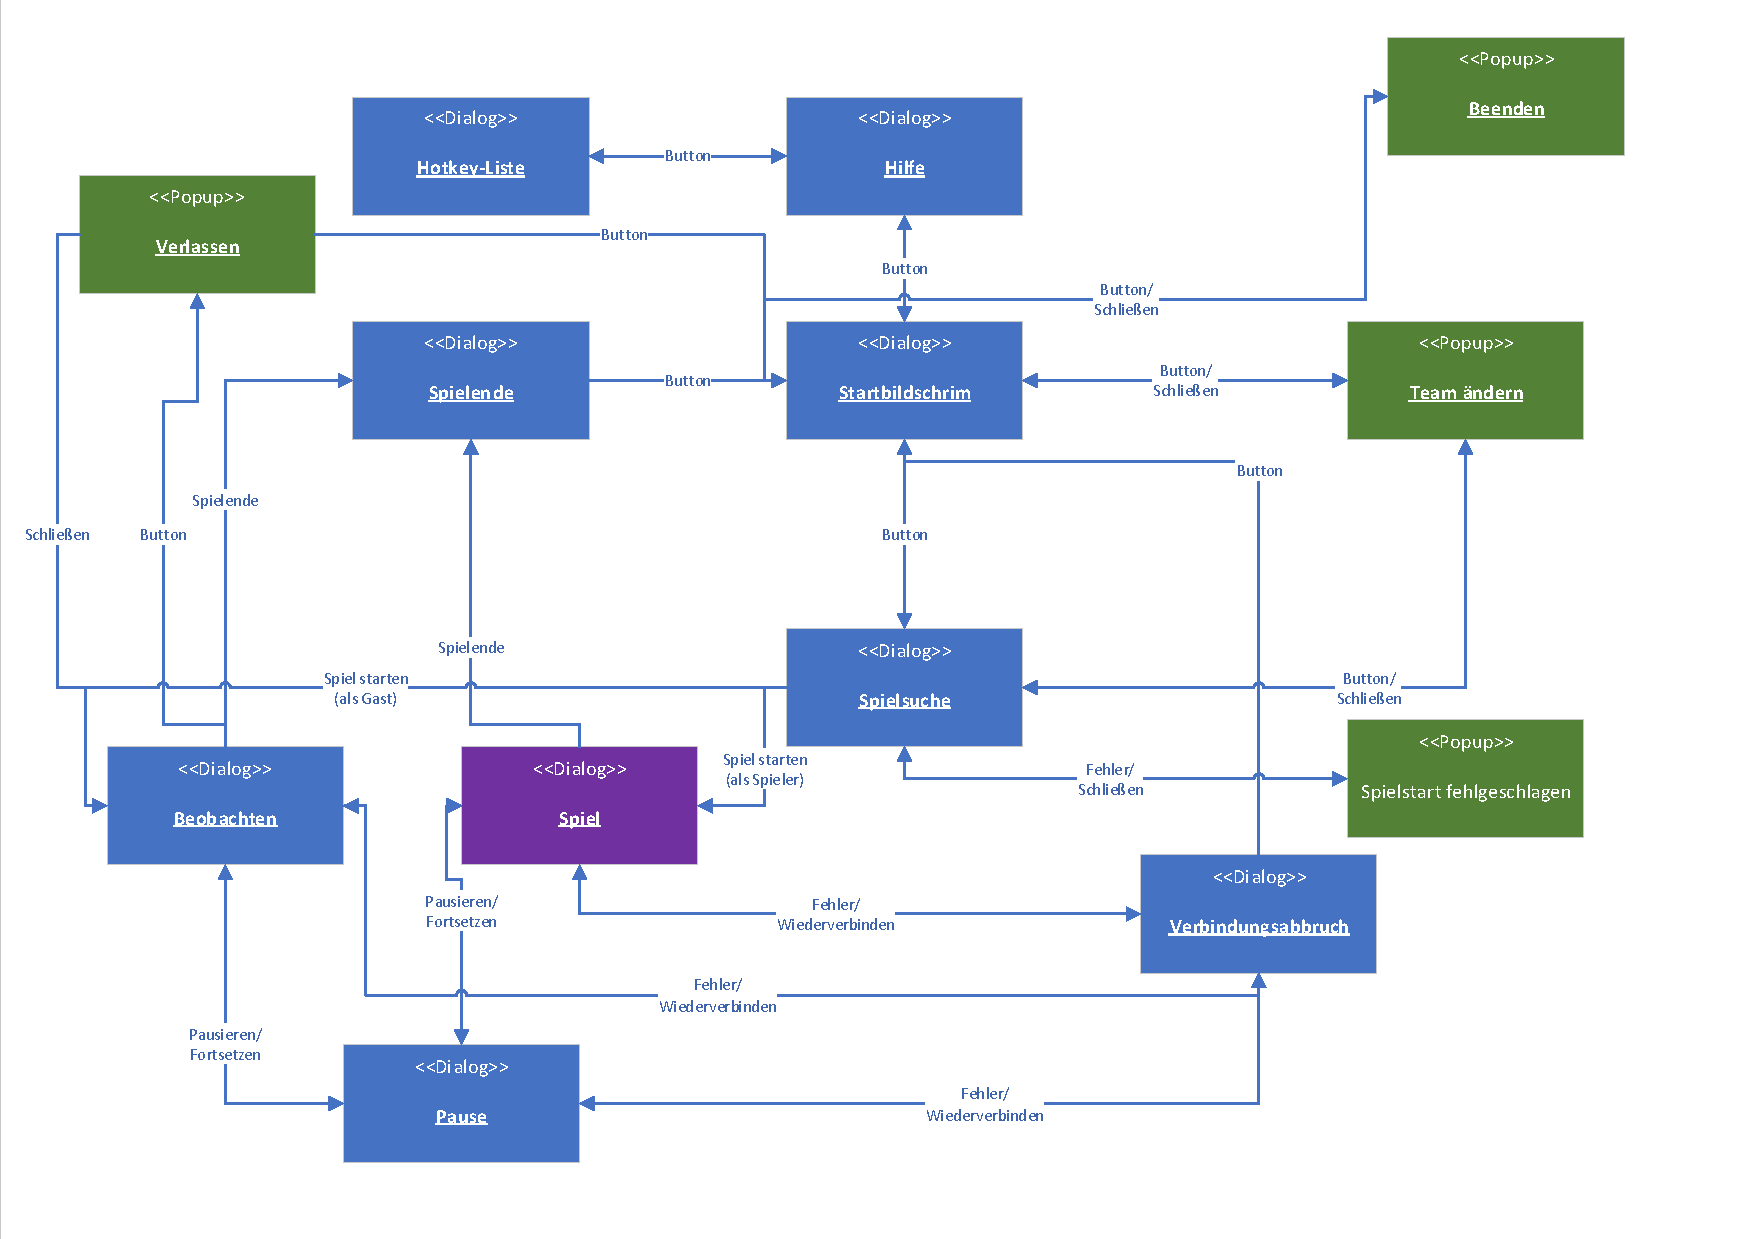
\includepdf[pages=-, scale=0.8, pagecommand={\subsubsection{Dialogstrukturdiagramme}}]{../Meilenstein03/images/Client_Hauptmenue.pdf}

    \subsection{Server}
    \subsection{Server}
Diese Komponente stellt den Server dar. Er hostet Spiele und enthält die Spiellogik. Zu Beginn wird er einmalig vom Systemadministrator gestartet und steht anschließend den Spielern von \textit{Fantastic Feasts} zur Verfügung.

\subsubsection{Schnittstellenarten}
Als Benutzerschnittstelle wird ein CLI verwendet. \textbf{Begründung:} Der Nutzer kommt mit dieser Komponente über keine Benutzerschnittstelle in Berührung. Deswegen spielen Look and Feel keine Rolle. Zusätzlich wird der Server nur einmal mit wenigen Parametern gestartet, benötigt zur Laufzeit dann keine weiteren Eingaben und muss auch keinerlei graphische Ausgabe zur Verfügung stellen, weswegen das CLI ausreicht.

\subsubsection{Dialoge}
Im Folgenden wird die Anforderung an den Server einem CLI-Dialog zugeordnet.

\begin{figure}[H]
    \centering
    \begin{tabular}{| l l l l |}
    \hline
    \textbf{Name} & \textbf{Typ} & \multicolumn{2}{l|}{\textbf{Abgedeckte Anwendungsfälle}} \\\hline
    ServerInit & CLI Befehl mit Params & FA74 & Serverkonfiguration einstellen \\\hline
    ServerRunning & Response & FA74 & Serverkonfiguration Feedback.\\\hline
    ServerError & Response & FA74 & Serverkonfiguration Feedback.\\\hline
    
    \end{tabular}
\end{figure}

\subsubsection{Dialogstruktur}  
Die Dialogstruktur des Servers lässt sich wie folgt beschreiben: \textbf{ServerInit:} Der Server lässt sich in der Konsole mit dem Namen der Server-Anwendung, dem Namen einer gültigen Partie-Konfiguration und einem Parameter aufrufen. Der Parameter ist die Port-Nummer, über die der Server erreichbar ist. Darauf gibt es zwei mögliches Antworten. \textbf{ServerRunning:} War die Initialisierung erfolgreich antwortet der Server mit einer entsprechenden Nachricht. \textbf{ServerEerror:} Im Falle eines Fehlers bei der Initialisierung wird mit einer Fehlernachricht geantwortet.
\subsubsection{Zulässige Optionen}
\begin{figure}[H]
    \centering
    \begin{tabular}{|p{2cm}|p{12cm} |}
        \hline
        Flag & Erklärung \\\hline
        -p & Legt die Portnummer fest.\\
        \hline
        -{}-help & Zeigt eine Liste möglicher Optionen an.\\\hline
    \end{tabular}
\end{figure}


    \subsection{Team- und Partiekonfigurator}
    Diese Komponente enthält einen Konfigurator, mit dem sich sowohl Quidditch-Teams, als auch Partie-Konfigurationen erstellen und bearbeiten lassen.

\subsubsection{Schnittstellenarten}
Als Benutzerschnittstelle wird, wie im Lastenheft vorgeschrieben, eine GUI verwendet. \textbf{Begründung:} Der Nutzer möchte alle Informationen zu einer gegebenen Konfiguration übersichtlich dargestellt bekommen und anhand dieser Darstellung direkt Änderungen vornehmen können. Hierfür ist eine GUI die intuitivste und sinnvollste Variante, da eine grafische Darstellung eine übersichtliche Visualisierung erlaubt und eine Änderung direkt anhand dieser Visualisierung möglich ist. 

\subsubsection{Dialoge}
Im Folgenden werden die bereits formulierten Anforderungen und Anwendungsfälle der Komponente den entsprechenden Dialogen zugeordnet.

\begin{figure}[H]
    \centering
    \begin{tabular}{| l l l l |}
    \hline
    \textbf{Name} & \textbf{Typ} & \multicolumn{2}{l|}{\textbf{Abgedeckte Anwendungsfälle}} \\\hline
    Konfiguratormenü & Dialog & QA18 & implizit aus Benutzerfreundlichkeit\\\hline
    Teammenü & Dialog & QA18 & implizit aus Benutzerfreundlichkeit\\\hline
    Team laden & Dialog & FA72 & Konfiguration öffnen \\\hline
    Teamkonfigurator & Dialog & FA70-72 & Konfiguration erstellen/bearbeiten\\\hline
    Team speichern & Dialog & FA72 & Konfiguration speichern \\\hline
    Partiemenü & Dialog & – & implizit, da Strukturierung erforderlich\\\hline
    Partiekonfiguration laden & Dialog & FA72 & Konfiguration öffnen \\\hline
    Partiekonfigurator & Dialog & FA70-72 & Konfiguration erstellen/bearbeiten\\\hline
    Partiefonfiguration speichern & Dialog & FA72 & Konfiguration speichern \\\hline
    Konfiguration erfolgreich & Popup & QA17-18 & Benutzerfreundlichkeit und Robustheit\\\hline
    Konfiguration ungültig & Popup & QA17-18 & Benutzerfreundlichkeit und Robustheit\\\hline
    \end{tabular}
\end{figure}

\subsubsection{Dialogstrukturdiagramme}    
\begin{figure}[H]
    \centering
    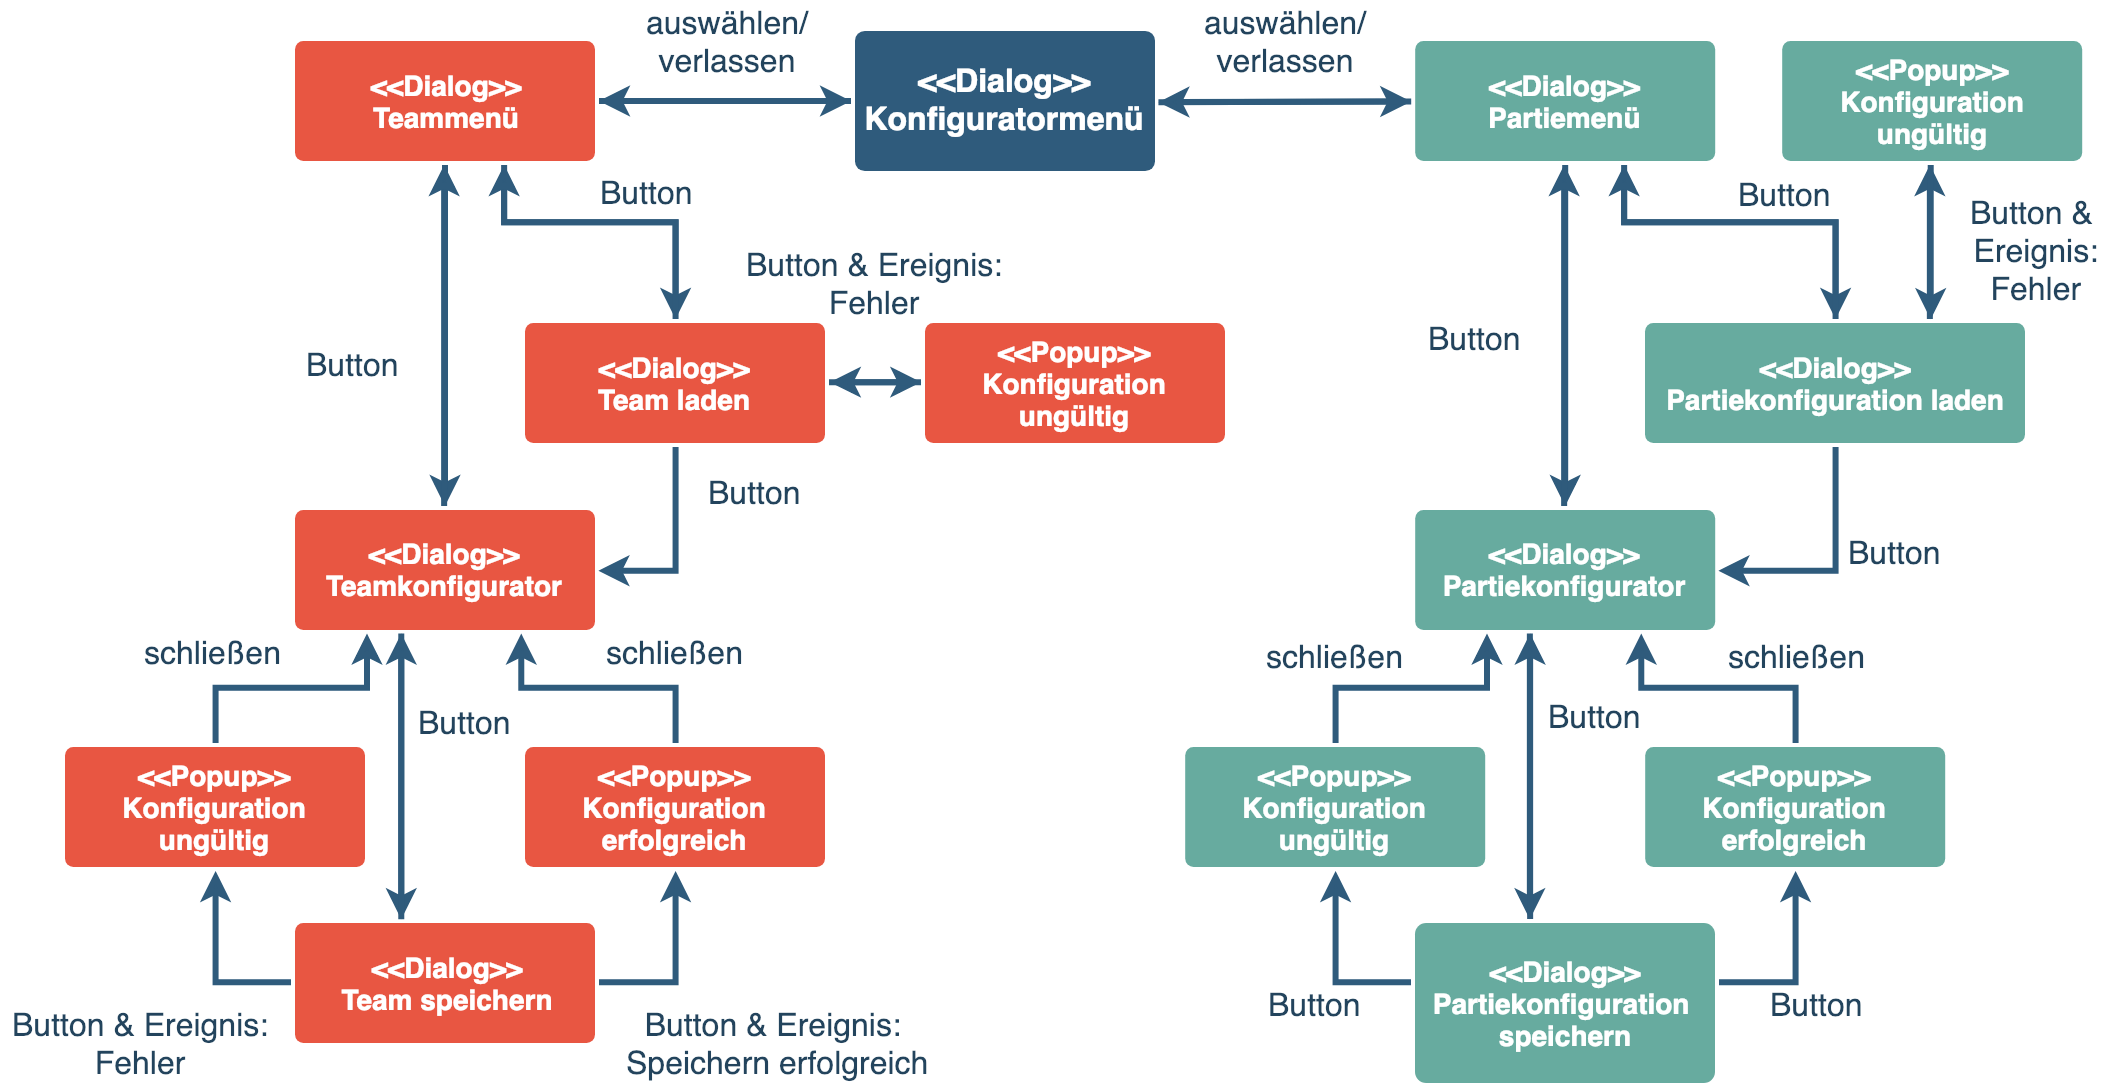
\includegraphics[width=\textwidth]{../Meilenstein03/images/dialogstruktur_konfigurator}
\end{figure}




    \subsection{KI-Client}
    Diese Komponente simuliert einen Menschlichen Gegner, der sich wie ein normaler Client bei einem Spielserver anmeldet und dann autonom seine Spielentscheidungen trifft.

\subsubsection{Schnittstellenarten}
Es besteht kein Grund, für diese Komponente eine grafische Oberfläche bereitzustellen, da die Anwendung zur Laufzeit keine Eingabe von einem menschlichen Benutzer erwartet und eine Partie mittels des Clients verfolgt werden kann. \\
Für eine Kommandozeilenanwendung ist es einfacher, Plattformunabhängigkeit sicherzustellen. Außerdem wird es damit problemlos möglich, den KI-Client aus einem anderen Programm zu starten. Beispielsweise kann dem Client eine Funktion hinzugefügt werden, gegen die KI zu spielen, ohne dass der Benutzer den KI-Client extern starten muss.\\

\subsubsection{Dialoge}
Im Folgenden werden die Anforderungen an den KI-Client einem CLI-Dialog zugeordnet.

\begin{figure}[H]
    \centering
    \begin{tabular}{| l l l p{4cm} |}
    \hline
    \textbf{Name} & \textbf{Typ} & \multicolumn{2}{l|}{\textbf{Abgedeckte Anwendungsfälle}} \\\hline
    Init & CLI Befehl mit Params & FA73 - FA75 & Schwierigkeit, Server- und Team-Konfiguration einstellen.\\\hline
	InitFailure & Response & FA73 - FA75 & Feedback.\\\hline
    WaitingForGame & Response & FA55 & Netzwerkschnittstelle, allgemeine Kommunikation.\\\hline
    Playing & Response & allgemein & Feedback.\\\hline
    AttemptingReconnect & Response & FA55 & Netzwerkschnittstelle, allgemeine Kommunikation.\\\hline
    ConnectionLost & Response & FA55 & Netzwerkschnittstelle, allgemeine Kommunikation.\\\hline
    \end{tabular}
\end{figure}

\subsubsection{Dialogstruktur}  
\textbf{Init:} Der KI-Client wird über die Kommandozeile gestartet. Serverkonfiguration, Team-Konfiguration, die maximale Anzahl an Reconnect-Versuchen und der Schwierigkeitsgrad werden beim Start der Anwendung mittels Kommandozeilenparametern gehandhabt. Der Server, mit dem sich der KI-Client verbinden soll wird als Argument übergeben. Die Team-Konfiguration und der Schwierigkeitsgrad können mittels Optionen verändert werden und nehmen ansonsten einen Standardwert an.\\
\textbf{InitFailure:} Wird eine ungültige Option angegeben, ist der Server nicht erreichbar oder wurde eine ungültige Team-Konfigurationsdatei geladen, so erscheint eine Fehlermeldung mit entsprechenden Hinweisen.\\
\textbf{WaitingForGame:} War die Initialisierung erfolgreich und der KI-Client konnte sich mit dem Server verbinden, so erscheint eine Nachricht, die darauf hinweist, dass noch auf den Beginn der Partie gewartet wird.\\
\textbf{Playing:} Während einer laufenden Partie wird ein Hinweis angezeigt.\\
\textbf{AttemptingReconnect:} Bei einem Verbindungsabbruch zeigt der KI-Client eine Meldung an und versucht automatisch, die Verbindung wiederherzustellen.\\
\textbf{ConnectionLost:} Konnte sich der KI-Client nicht innerhalb der angegebenen Anzahl von Versuchen erneut mit dem Server verbinden, so erscheint eine Fehlermeldung und das Programm beendet sich.\\
Der KI-Client beendet sich außerdem nach Abschluss einer Partie durch ein reguläres Spielende. 

\subsubsection{Zulässige Optionen:}
\begin{figure}[H]
    \centering
    \begin{tabular}{|p{2cm}|p{12cm} |}
        \hline
        Flag & Erklärung \\\hline
        -s & Legt den Schwierigkeitsgrad fest.\\
        & Akzeptiert eine ganze Zahl zwischen 0 und 2, wobei 0 für einfach,\\
        & 1 für mittelschwer und 2 für schwer steht.\\
        & Bei einer ungültigen Eingabe wird eine Fehlermeldung ausgegeben.\\\hline
        -t & Legt die Team-Konfiguration fest.\\
        & Akzeptiert einen String als Pfad zu einer JSON-Datei.\\
        & Existiert der angegebene Pfad nicht oder ist die Datei keine gültige Konfigurationsdatei,\\
        & wird eine entsprechende Fehlermeldung ausgegeben.\\\hline
		-r & Reconnects: Spezifiziert, wie oft der KI-Client versucht, die Verbindung nach einem Verbindungsabbruch 
		wiederherzustellen. Standardwert ist 5.\\\hline
        -{}-help & Zeigt eine Liste möglicher Optionen an.\\\hline
    \end{tabular}
\end{figure}

    
	\section{Grafische Gestaltung und Nutzungskonzept}
    \subsection{Client}
    \subsection{Client}

    \subsubsection{Spielansicht für einen Spieler}

    \begin{figure}[H]
        \centering
        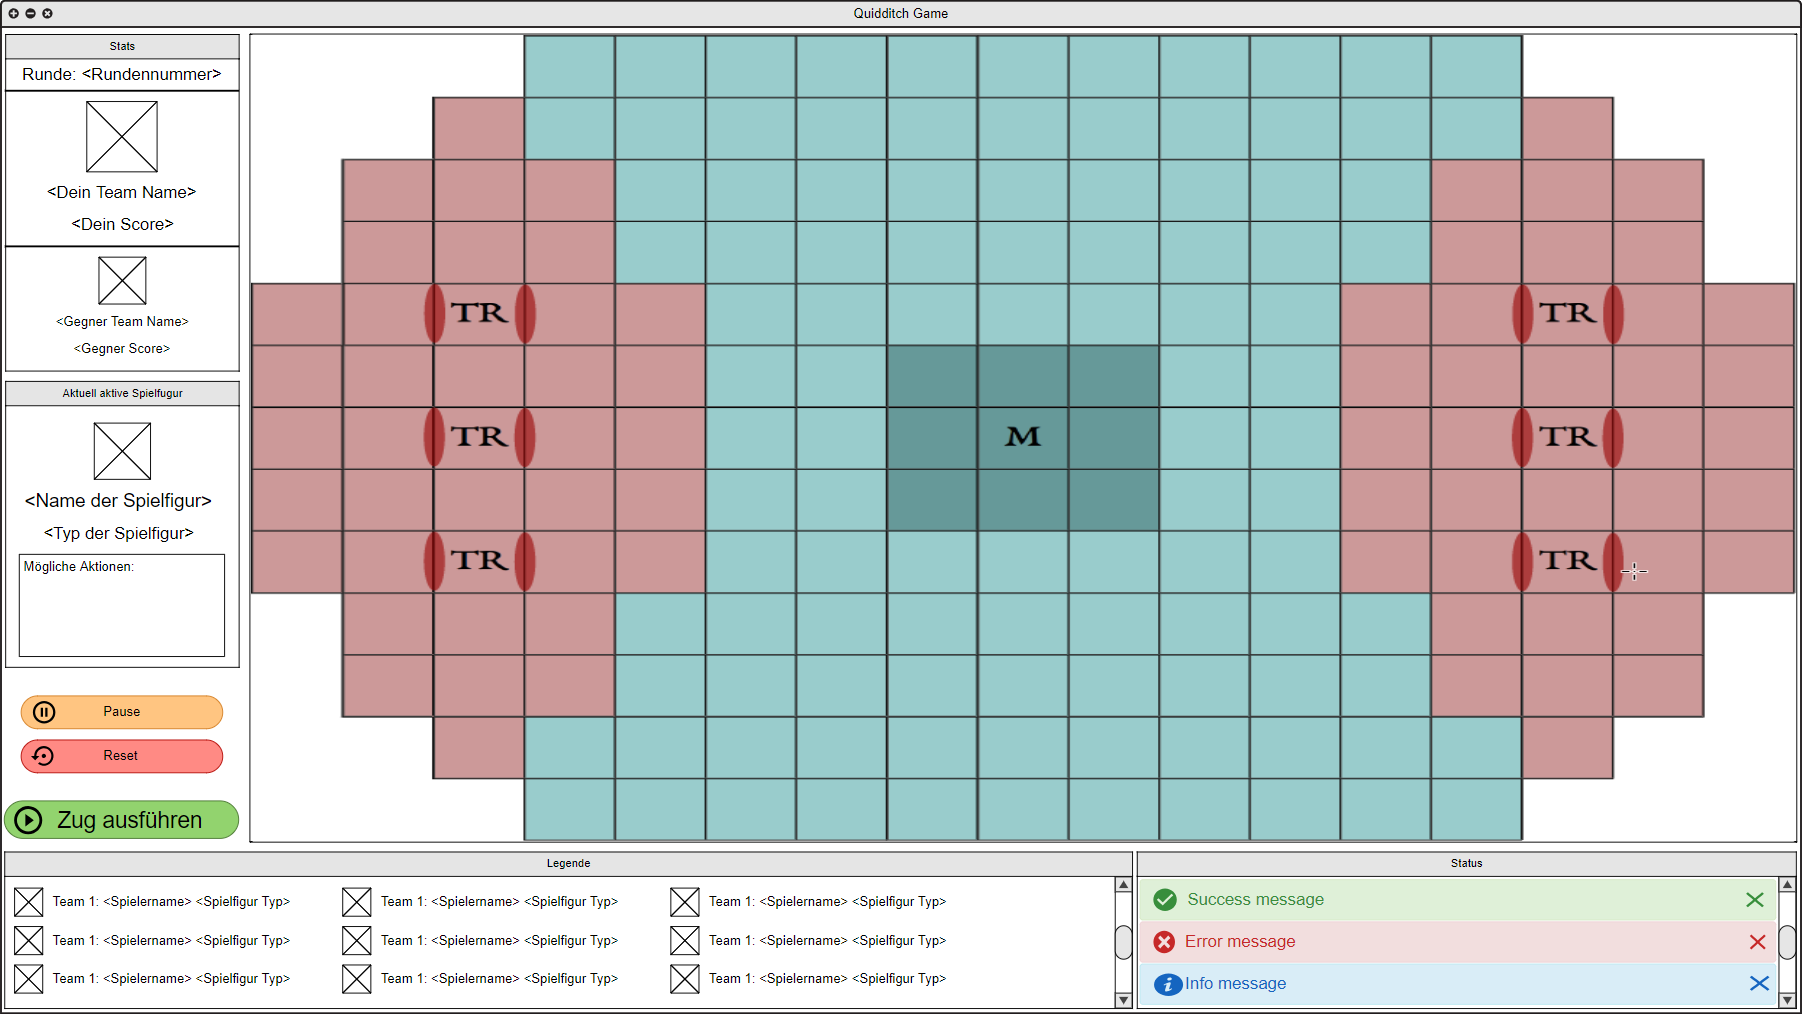
\includegraphics[width=\textwidth]{images/InGamePlayer.PNG}
    \end{figure}

    In der Spielansicht kann ein Spieler das aktuelle Spielgeschehen verfolgen und sein Züge ausführen. Dabei ist die Oberfläche in mehrere Teile unterteilt.\\
    Im \textit{Stats} Bereich werden grundlegende Informationen über die aktuelle Partie und die beiden Teams dargestellt. Das Team, das an oberster Position steht, ist momentan am Zug. Der darunter liegende Bereich ist der \textit{Fan} Bereich. Hier kann der Spieler auswählen, ob und welcher Fan eine Aktion ausführen soll. Darunter befinden sich drei Buttons mit dem entweder das Spiel \textit{pausiert} werden , alle Veränderungen die man in der aktuellen Runde getätigt hat \textit{zurücksetzen} oder seinen Zug endgültig \textit{ausführen} kann. Am unteren Rand der Oberfläche ist eine \textit{Legende} mit einer Übersicht über alle Spielfiguren des eigenen und des gegnerischen Teams zu sehen. Daneben befindet sich ein Feld, in dem Statusmeldungen angezeigt werden können. Beispiele für solche Statusmeldungen sind zum Beispiel eine Benachrichtigung über ein Faul oder über das erfolgreiche Ausführen eines Spielzuges. Der größte Teil der Oberfläche nimmt dass eigentliche Spielfeld ein. Hier werden alle Spielfiguren in den Feldern angezeigt auf denen sie sich gerade befinden. Ist man am Zug und klickt auf einen Spieler, so werden alle Züge, die von der Spielfigur ausgeführt werden können farblich hervor gehoben. Der Spieler kann diese Aktionen dann durch weitere Klicks ausführen und die Prozedur gegebenenfalls für weitere Spielfiguren wiederholen. Ist man nicht am Zug so werden alle Eingabemöglichkeiten, mit Ausnahme des \textit{Pause} Buttons deaktiviert.
    

    \subsubsection{Spielansicht für einen Beobachter}
        
    \begin{figure}[H]
        \centering
        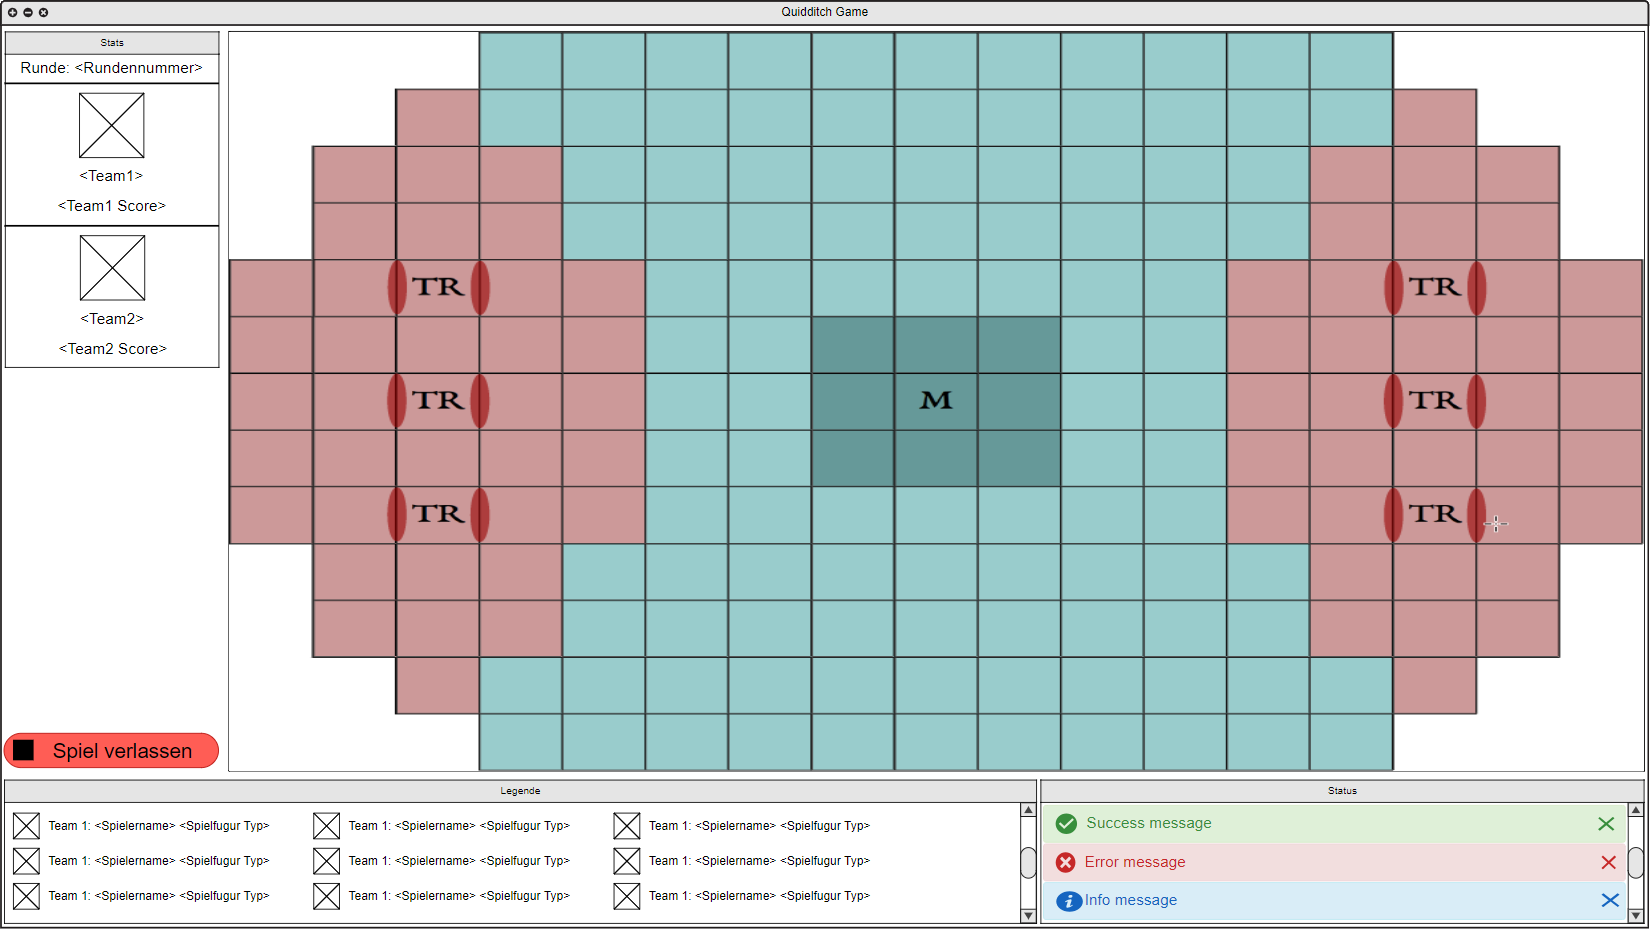
\includegraphics[width=\textwidth]{images/InGameObserver.PNG}
    \end{figure}

    In der Spielansicht kann ein Beobachter eine Partie wischen zwei anderen Gegnern passiv verfolgen. Die Oberfläche ist im wesentlichen gleich aufgebaut wie die Oberfläche, die die Spieler sehen. Jedoch sind beim Beobachter alle Felder die zur Eingabe dienen deaktiviert und teilweise ausgeblendet. Die einzige Interaktion, welche durch einen Button ermöglicht wird ist das vorzeitige \textit{verlassen} einer Partie.
    
    \subsubsection{Startbildschirm}
\begin{figure}[H]
	\centering
	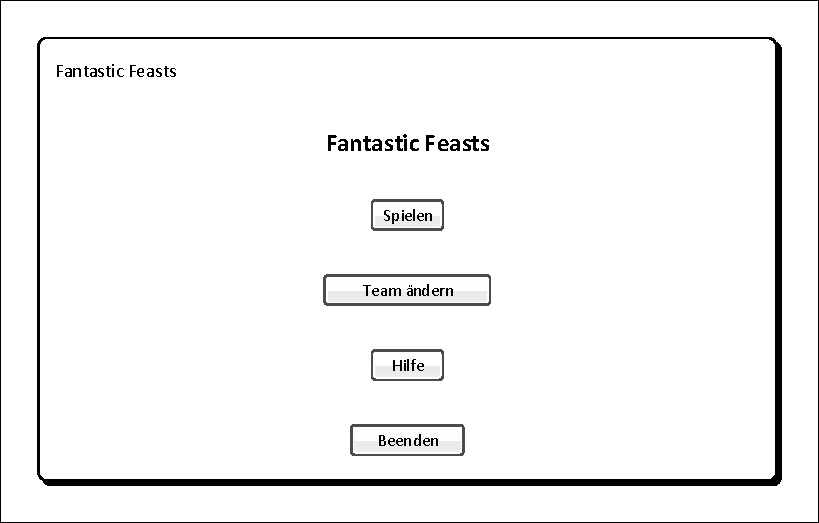
\includegraphics[scale=0.8]{images/Startbildschirm.pdf}
\end{figure}

Dieser Dialog erscheint nach Start der Anwendung. Der \glqq{}Spielen\grqq{}-Button öffnet den Spielsuche-Dialog. Der \glqq{}Team ändern\grqq{}-Button öffnet das \glqq{}Team ändern\grqq{}-Popup. Der \glqq{}Hilfe\grqq{}-Button öffnet den Hilfe-Dialog. Der \glqq{}Beenden\grqq{}-Button öffnet ein Bestätigungs-Popup und beendet bei positiver Antwort die Anwendung.

\subsubsection{Spielsuche}
\begin{figure}[H]
	\centering
	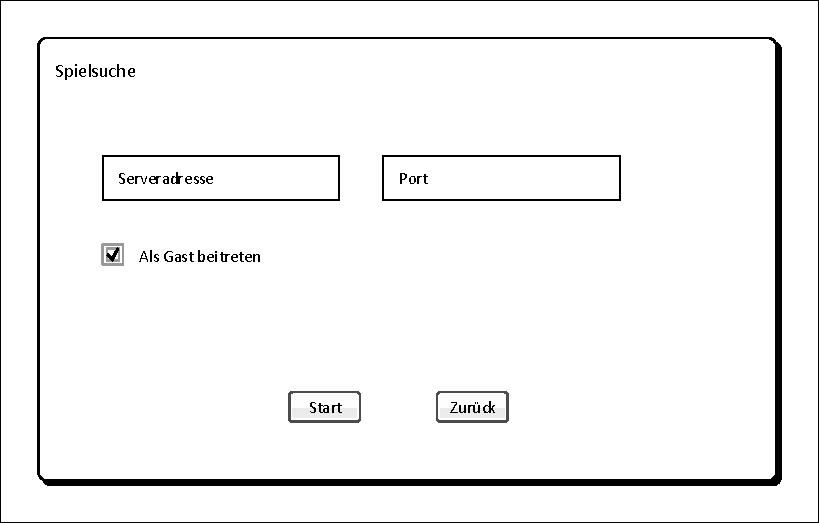
\includegraphics[scale=0.8]{images/Spielsuche.pdf}
\end{figure}

Der Benutzer gibt zuerst die Adresse und den Port des Spielservers und, mit dem er sich verbinden möchte. Wenn er die Partie beobachten will, wählt er \glqq{}Als Gast beitreten\grqq{} aus. Drückt er anschließend auf den \glqq{}Start\grqq{}-Button, versucht sich der Client mit dem angegebene Server zu verbinden. Mit dem \glqq{}Zurück\grqq{}-Button kann man zurück auf den Startbildschirm gelangen.
	
\subsubsection{Hilfe}
\begin{figure}[H]
	\centering
	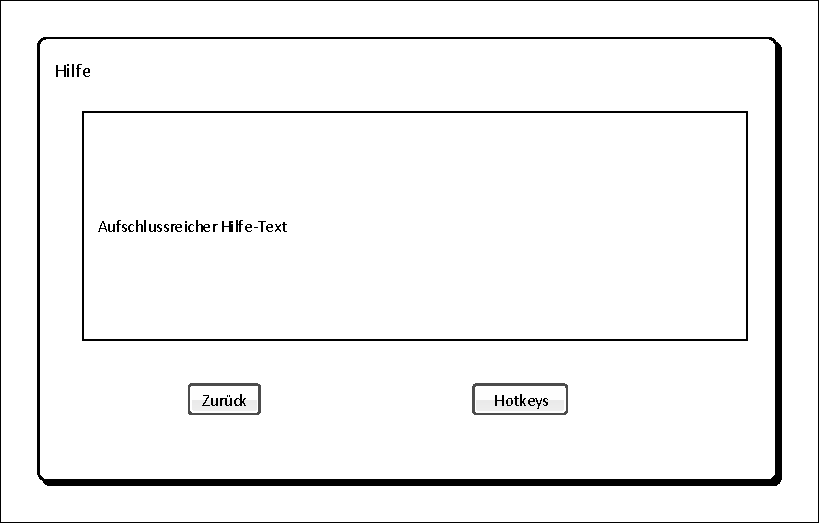
\includegraphics[scale=0.8]{images/Hilfe.pdf}
\end{figure}

In einem großen Textfeld, gegebenenfalls mit Scrollbar, wird ein Hilfetext angezeigt. Der \glqq{}Zurück\grqq{}-Button öffnet den Startbildschirm, der \glqq{}Hotkey\grqq{}-Button den Hotkey-Dialog.

\subsubsection{Hotkeys}
\begin{figure}[H]
	\centering
	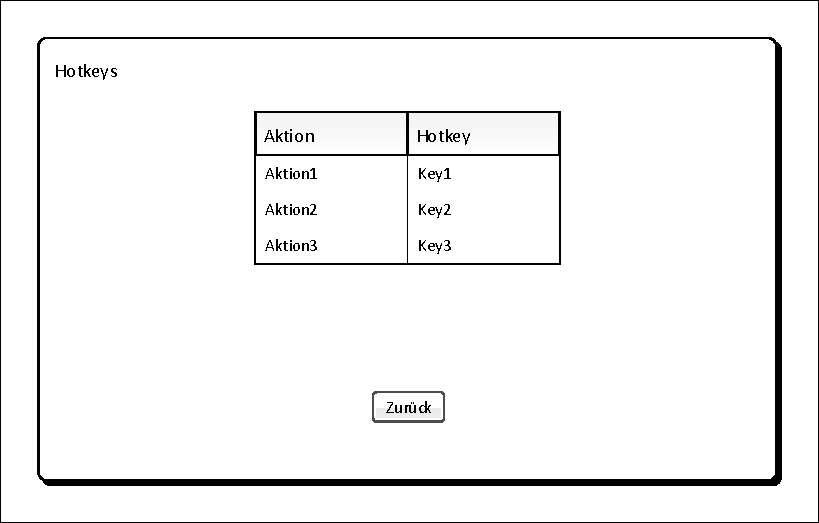
\includegraphics[scale=0.8]{images/Hotkeys.pdf}
\end{figure}

Hier werden alle verfügbaren Hotkeys in Tabellenform aufgelistet. Der \glqq{}Zurück\grqq{}-Button öffnet den Hilfe-Dialog.

\subsubsection{Team ändern}
\begin{figure}[H]
	\centering
	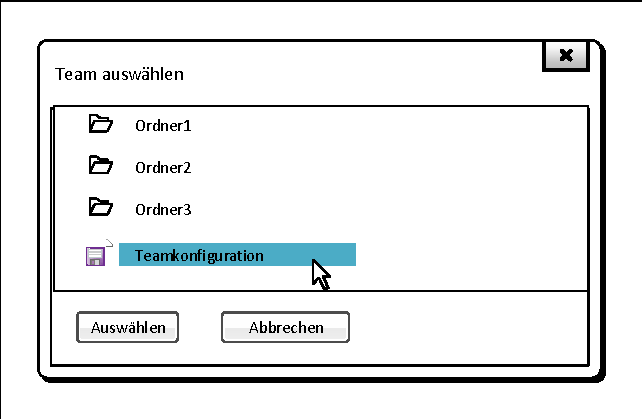
\includegraphics[scale=0.8]{images/Teamauswahl_Popup.pdf}
\end{figure}

In diesem Popup kann der Benutzer durch sein Dateisystem navigieren und eine JSON-Datei auswählen. Hat er eine gültige Datei ausgewählt und betätigt den \glqq{}Auswählen\grqq{}-Button, wird das Popup geschlossen und die Team-Konfiguration für das Spiel verwendet. Der \glqq{}Abbrechen\grqq{}-Button schließt das Popup und es werden keine Änderungen vorgenommen.

\subsubsection{Bestätigungsaufforderung}
\begin{figure}[H]
	\centering
	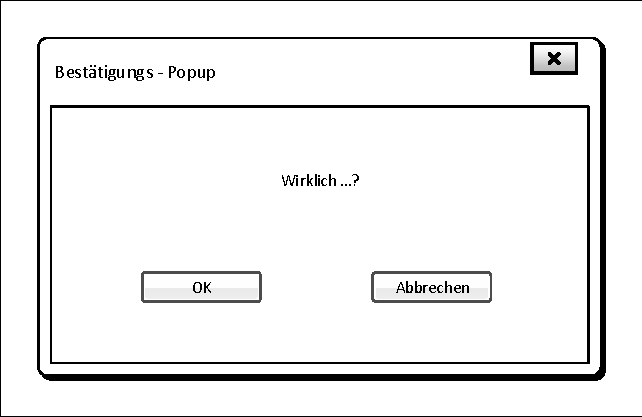
\includegraphics[scale=0.8]{images/OK_Popup.pdf}
\end{figure}

Dieser Aufbau wird für die Popups \glqq{}Beenden\grqq{} und \glqq{}Verlassen\grqq{} verwendet. Der \glqq{}Abbrechen\grqq{}-Button schließt das Popup und der Benutzer gelangt zurück in den Dialog, in dem er vor Öffnen des Popups war. Der "OK"-Button führt dazu, dass eine Aktion ausgeführt wird.

\subsubsection{Fehler}
\begin{figure}[H]
	\centering
	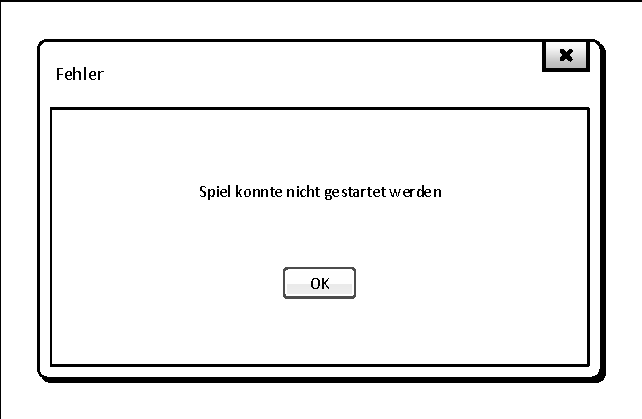
\includegraphics[scale=0.8]{images/Fehler_Popup.pdf}
\end{figure}

Dieser Aufbau wird für das Popup \glqq{}Spielstart fehlgeschlagen\grqq{} verwendet. Der angezeigt Text richtet sich nach dem aufgetretenen Fehler. Der \glqq{}OK\grqq{}-Button schließt das Popup.

\subsubsection{Pause}
\begin{figure}[H]
	\centering
	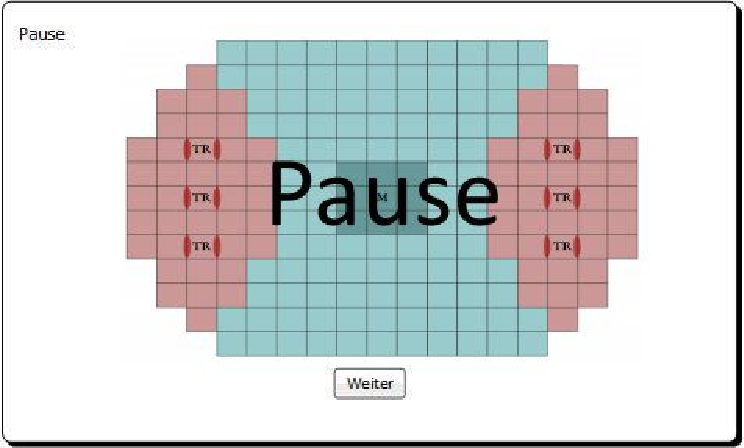
\includegraphics[scale=0.8]{images/Pause.pdf}
\end{figure}

Wird angezeigt, wenn das Spiel von einem Spieler pausiert wird. Der \glqq{}Weiter\grqq{}-Button setzt die Partie fort und kann nicht von einem Gast betätigt werden.

\subsubsection{Verbindungsabbruch}
\begin{figure}[H]
	\centering
	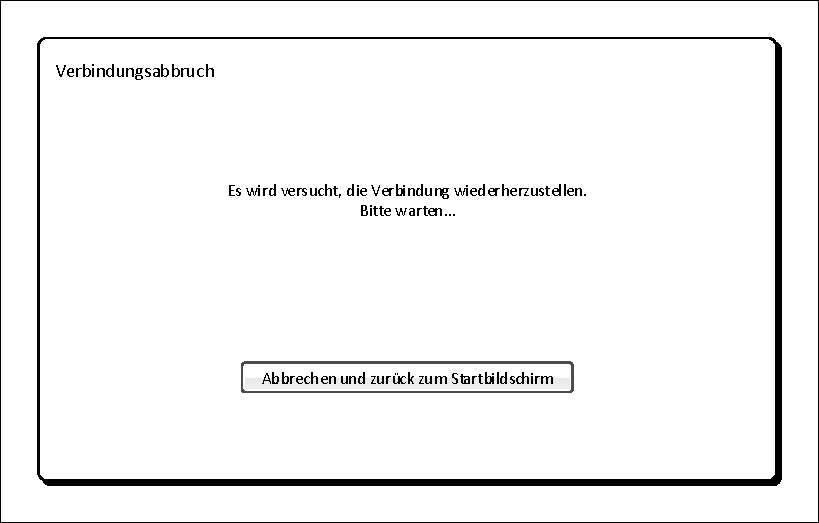
\includegraphics[scale=0.8]{images/Verbindungsabbruch.pdf}
\end{figure}

Im Falle eines Verbindungsabbruchs zwischen Client und Server wird dieser Dialog angezeigt. Wird die Verbindung wiederhergestellt, gelangt der Benutzer automatisch wieder zurück in den vorherigen Dialog. Alternativ kann er durch betätigen des Buttons zum Startbildschirm gelangen. Ist er ein Spieler, kann er die Partie nicht weiterführen und sein Gegner gewinnt nach Ablauf einer Zeitdauer die Partie.

\subsubsection{Spielende}
\begin{figure}[H]
	\centering
	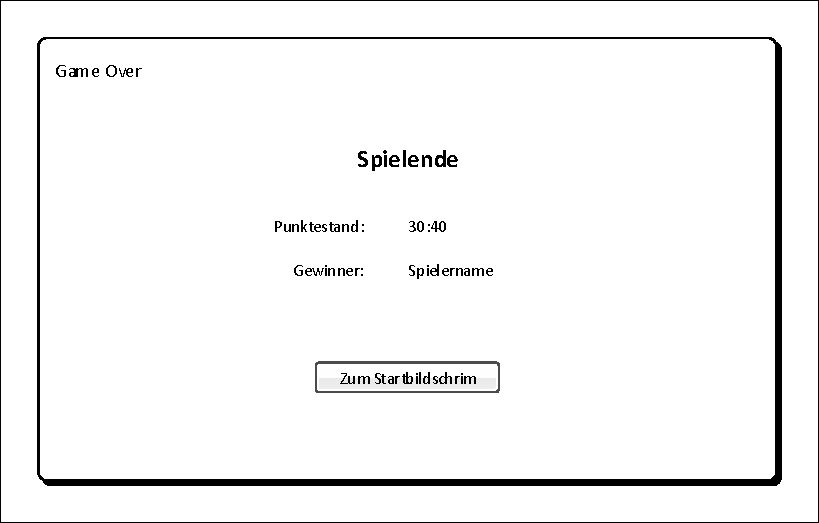
\includegraphics[scale=0.8]{images/Spielende.pdf}
\end{figure}

Bei Spielende wird dieser Dialog geöffnet. Hier werden der Punktestand bei Spielende und der Name des Gewinners angezeigt. Der Button öffnet den Startbildschirm-Dialog.
	
    \subsection{Server}
    \subsection{Server}
	\subsubsection{ffServerInit}
	\lstset{language=bash} 
	\begin{lstlisting}[frame=single]
  	$ ffserver 1230 standard_partie.json
  	... pending
	\end{lstlisting}
	Das Beispiel für einen Aufruf des Servers mit entsprechenden Parametern dar.
	
	\subsubsection{ffServerRunning}
	\lstset{language=bash} 
	\begin{lstlisting}[frame=single]
  	Fantastic Feasts server is running on Port 1230 ...
	\end{lstlisting}
	Im Falle einer erfolgreichen Initialisierung wird dies dem Systemadministrator über diese Nachricht mitgeteilt. In dieser Nachricht können weitere Informationen über den initialisierten Server verpackt werden.
	
	\subsubsection{ffServerError}
	\lstset{language=bash} 
	\begin{lstlisting}[frame=single]
  	Error: Initialization failed
	\end{lstlisting}
	Im Falle eines Fehlers bei der Initialisierung wird der Systemadministrator mit dieser Fehlermeldung benachrichtigt.


	
    \subsection{Team- und Partiekonfiguraton}
    \subsubsection{Konfiguratormenü}

    \begin{figure}[H]
        \centering
        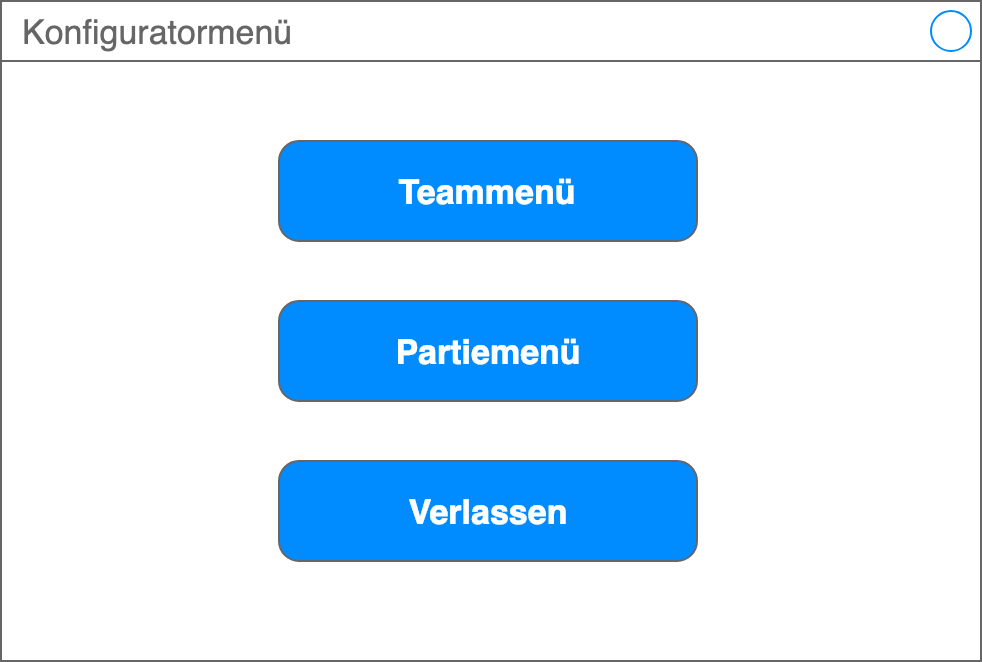
\includegraphics[width=\textwidth/2]{../Meilenstein03/images/konfiguratormenue}
    \end{figure}

    Über das Konfiguratormenü kann eine Auswahl zwischen dem Teammenü und dem Partiemenü über die entsprechenden Buttons getroffen werden. Diese führen zu den Menüs der jeweiligen Konfiguratoren. Über den Button \textit{Verlassen} kann der Konfigurator verlassen werden.

    \subsubsection{Teammenü}
    \begin{figure}[H]
        \centering
        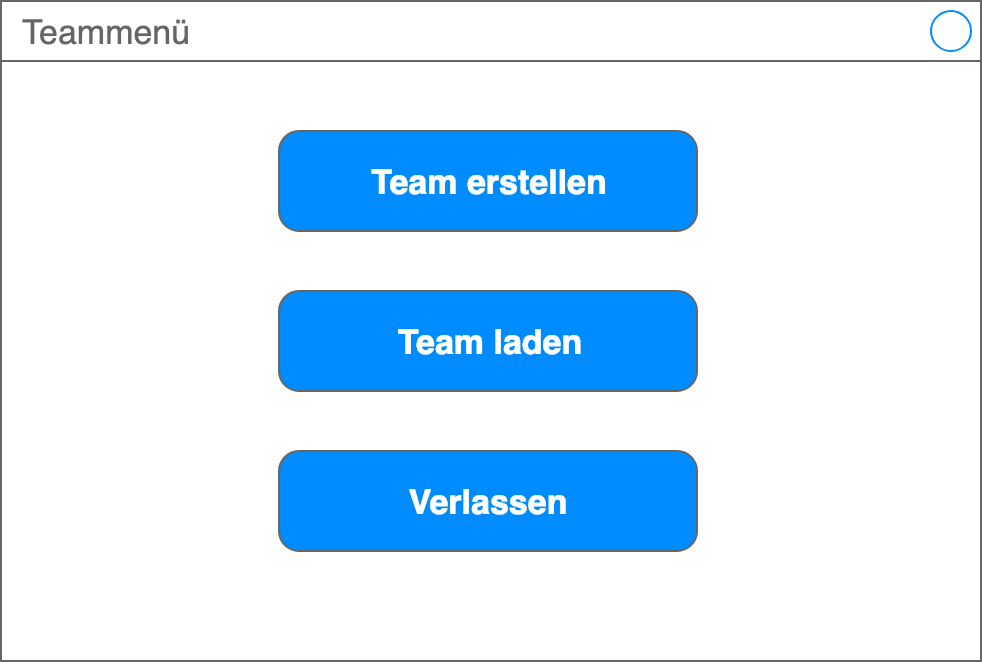
\includegraphics[width=\textwidth/2]{../Meilenstein03/images/teammenue}
    \end{figure}

    Über das Teammenü kann eine Auswahl zwischen dem Laden und dem Erstellen einer Teamkonfiguration getroffen werden. Das erfolgt über die entsprechenden Buttons. Über den Button \textit{Verlassen} kann das Teammenü verlassen werden.

    \subsubsection{Team bzw. Partiekonfiguration laden}

    \begin{figure}[H]
        \centering
        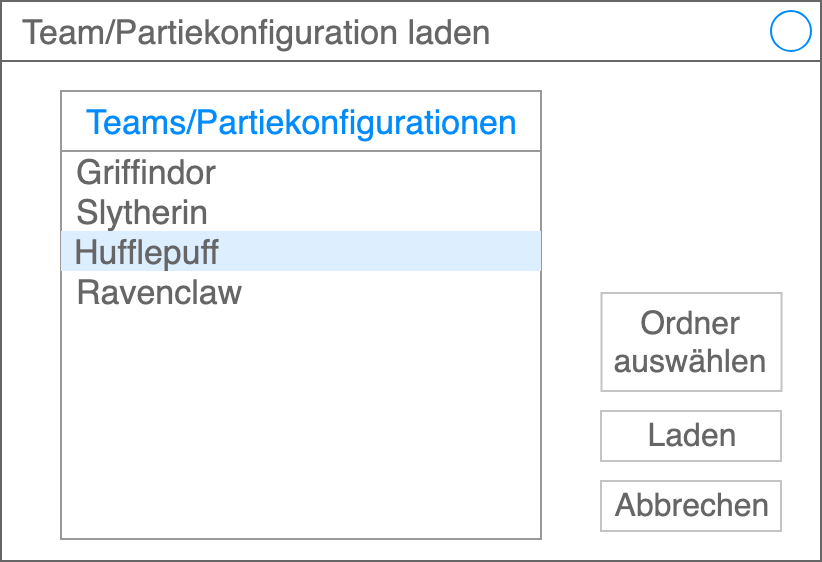
\includegraphics[width=\textwidth/2]{../Meilenstein03/images/laden}
    \end{figure}

    Über diesen Dialog kann eine bereits vorhanden Konfigurationsdatei ausgewählt und im Konfigurator geladen werden. Das erfolgt über ein Dateiauswahlelement und die entsprechenden Buttons. Über den Button \textit{Abbrechen} gelangt man zurück zu den entsprechenden Menüs. Da das Laden einer Teamkonfiguration nahezu identisch zum Laden einer Partiekonfiguration ist, wurde diese beiden Fälle in einem zusammen gefasst. Sollte eine zu ladende Konfigurationsdatei ungültig sein, öffnet sich das Popup \textit{Konfiguration ungültig}.


    \subsubsection{Teamkonfigurator}

    \begin{figure}[H]
        \centering
        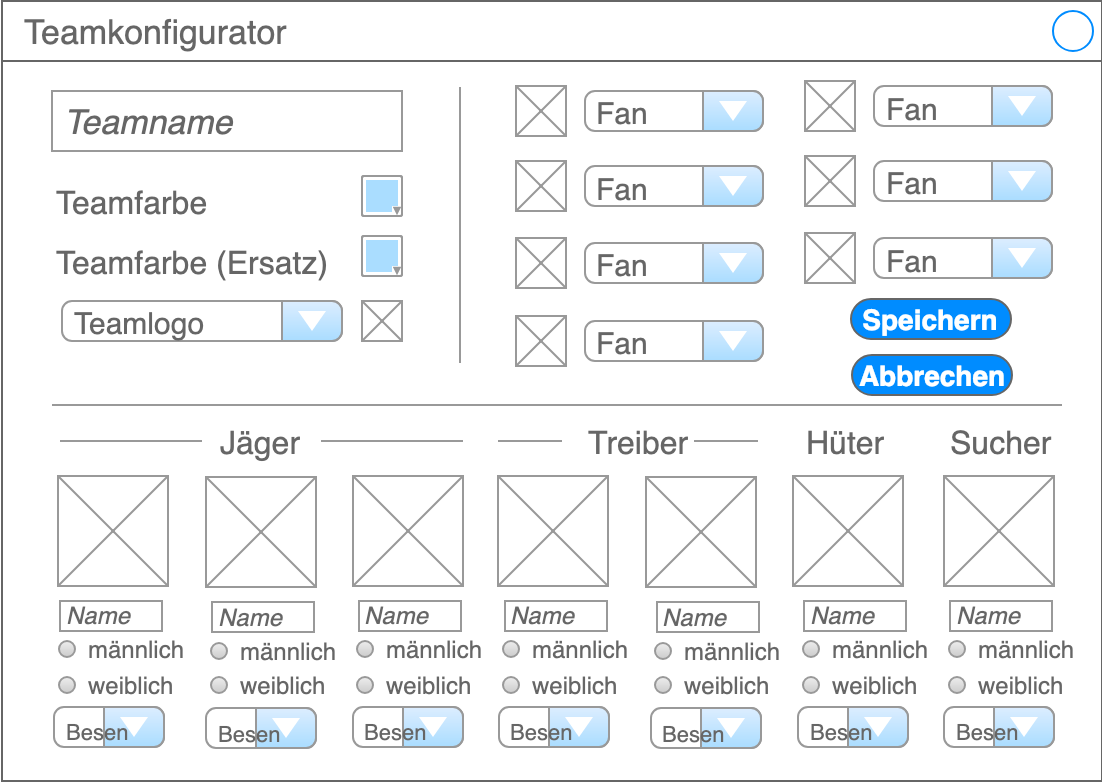
\includegraphics[width=\textwidth]{../Meilenstein03/images/teamkonfigurator}
    \end{figure}

    Im Teamkonfigurator können alle Parameter eines Teams eingestellt werden. Team- und Spielernamen lassen sich durch ein Textfeld bearbeiten. Teamfarben sind über eine Farbauswahl einstellbar. Das Teamlogo lässt sich aus einer Liste vorhandener Logos auswählen. Die Kästen mit den Kreuzen dienen als Platzhalter für Icons, die die verschiedenen Fans und Spieler darstellen und somit unterscheidbar machen. Fans sowie Besen der Spieler sind über eine Dropdown-Auswahl einstellbar. Das Geschlecht der Spieler lässt sich über Radio-Buttons einstellen. Bei jeder Änderung werden die entsprechenden Bedingungen für eine gültige Konfiguration geprüft und der Nutzer erhält visuelles Feedback (z. B. in Form von roter Schriftfarbe in den entsprechenden Feldern). Über den Button \textit{Abbrechen} lässt sich der Konfigurator jederzeit verlassen. Ist eine gültige Auswahl eingestellt, kann die Konfiguration über \textit{Speichern} in einem separaten Speicherdialog persistiert werden.

    \subsubsection{Team bzw. Partiekonfiguration speichern}

    \begin{figure}[H]
        \centering
        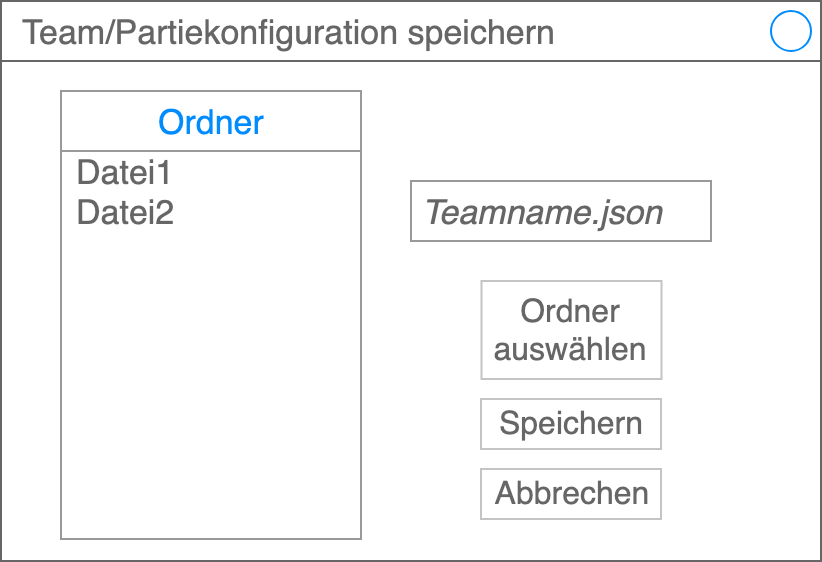
\includegraphics[width=\textwidth/2]{../Meilenstein03/images/speichern}
    \end{figure}

    In diesem Dialog kann Dateiname und Speicherort der Konfiguration festgelegt werden. Der Button \textit{Abbrechen} bringt den Nutzer direkt zurück in den entsprechen Konfigurator. Durch Klicken auf den Button \textit{Speichern} wird die Datei mit dem gewählten Namen und Speicherort gespeichert.

    Wurde versucht eine Konfiguration mit ungültigen Parametern zu speichern oder trat beim Speichervorgang ein Fehler auf, wird der Nutzer über dieses Popup darüber informiert. Der \textit{Ok}-Button führt zurück zum entsprechenden Konfigurator.

    \subsubsection{Konfiguration erfolgreich}

    \begin{figure}[H]
        \centering
        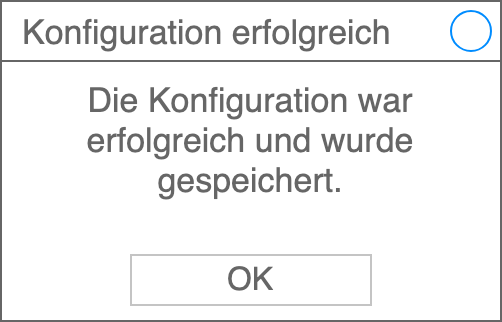
\includegraphics[width=\textwidth/2]{../Meilenstein03/images/konfiguration_erfolgreich}
    \end{figure}

    Wenn alle Paramter einer Konfiguration gültig waren, wird dieser Dialog angezeigt. Der \textit{Ok}-Button führt zurück zum entsprechenden Menü.

    \subsubsection{Konfiguration ungültig}

    \begin{figure}[H]
        \centering
        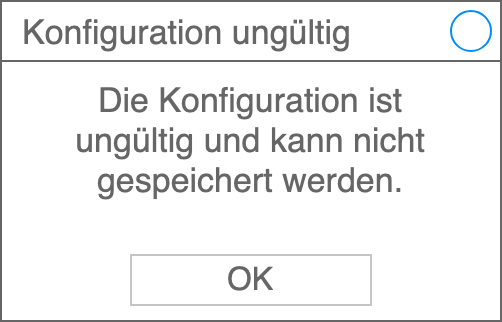
\includegraphics[width=\textwidth/2]{../Meilenstein03/images/konfiguration_ungueltig}
    \end{figure}

    Wurde versucht eine Konfiguration mit ungültigen Parametern zu speichern oder trat beim Speichervorgang ein Fehler auf, wird der Nutzer über dieses Popup darüber informiert. Der \textit{Ok}-Button des Popups führt zurück zum entsprechenden Dialog.

    \subsubsection{Partiemenü}

    \begin{figure}[H]
        \centering
        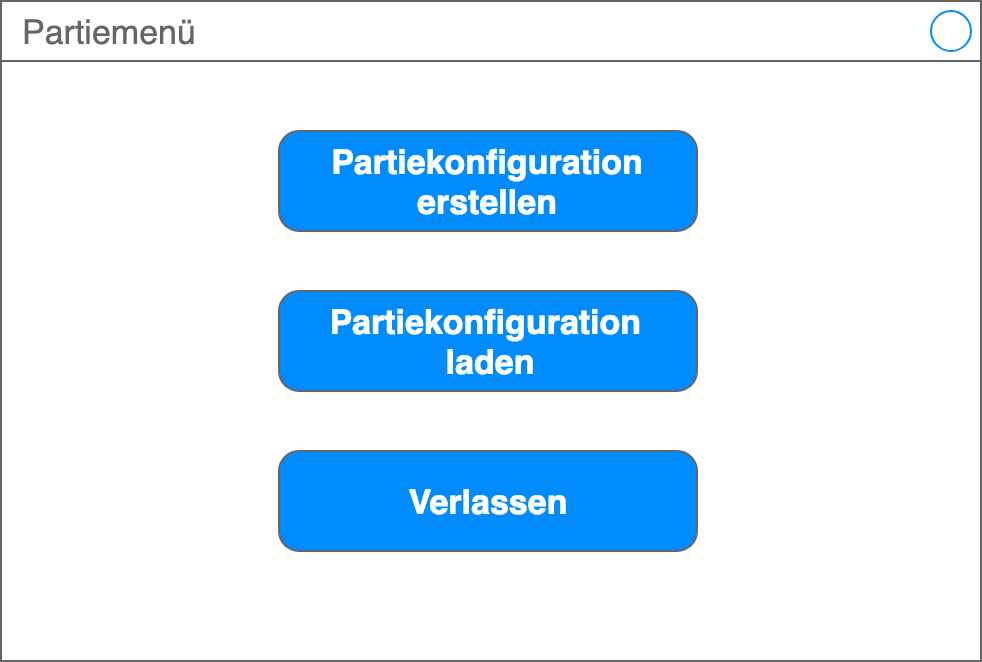
\includegraphics[width=\textwidth/2]{../Meilenstein03/images/partiemenue}
    \end{figure}

    Über das Partiemenü kann eine Auswahl zwischen dem Laden und dem Erstellen einer Partiekonfiguration getroffen werden. Das erfolgt über die entsprechenden Buttons. Über den Button \textit{Verlassen} kann das \textit{Partiemenü} verlassen werden.

    \subsubsection{Partiekonfigurator}

    \begin{figure}[H]
        \centering
        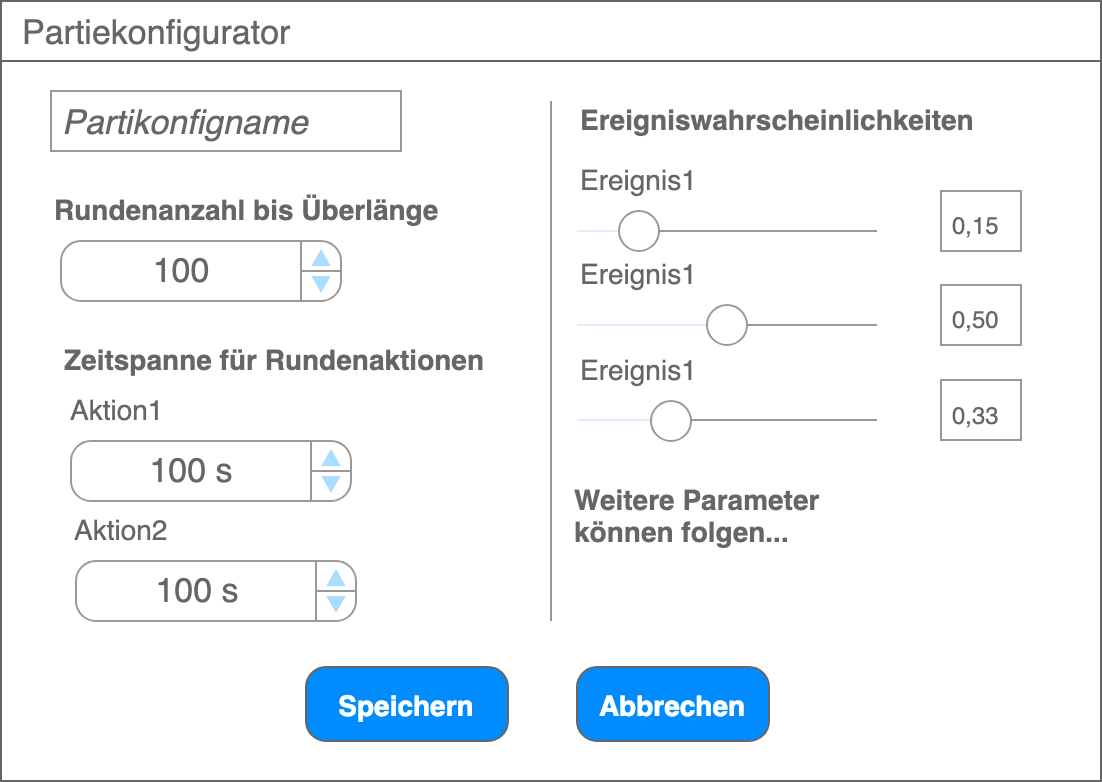
\includegraphics[width=\textwidth]{../Meilenstein03/images/partiekonfigurator}
    \end{figure}

    Im Partiekonfigurator können alle Paramter für eine gültige Partiekonfigurationsdatei eingestellt werden. Dazu gehören unter anderem die Rundenzahl, bis Überlänge erreicht ist, die Zeitspannen für die jeweiligen Spielaktionen und Ereigniswahrscheinlichkeiten. Je nach Art des Parameteres sind Spinner, Slider, Textfelder oder im weiteren Verlauf der Implementierung noch andere Auswahlelemente vorhanden.

    Über den Button \textit{Speichern} gelangt man in den \textit{Partiekonfiguration speichern}-Dialog. Der Button \textit{Abbrechen} führt zurück ins \textit{Partiemenü}.

	

    \section{Nutzungskonzept}
    %TODO
    \section{Datenmodell}
    %TODO
    \section{Funktionen}
    %TODO

    \part{Randbedingungen}
    \section{Qualität}
    \subsection{Nicht funktionale Anforderungen}

\qanf 	{Plattformunabhängigkeit}
        {Der Client und der Team-Konfigurator soll auf mindestens einer gängigen Computerbetriebssystem-Plattform (z.B. Linux, Windows) uneingeschränkt benutzbar sein. Des weiteren soll die Serveranwendung und der KI-Client auf mindestens zwei gängigen Computerbetriebssystem-Plattformen (z.B. Linux, Windows) uneingeschränkt benutzbar sein.}
        {Die Plattformunabhängigkeit ist von großer Bedeutung, da die Anwendungen auf möglichst vielen Zielsystemen funktionieren sollen um die Menge an Endnutzer so wenig wie möglich einzuschränken.}
        {Programmiersprache, Docker-Container}
        {+}
        {Nutzer, Entwickler}

\qanf 	{Version-Controlling}
        {Beim Verwalten des Quellcodes soll ein Git basiertes Version-Controlling Werkzeug (\textit{GitHub / GitLab}) verwendet werden.}
        {Durch das Verwenden eines Versionierungswerkzeuges wird das zusammenarbeiten unterschiedlicher Entwickler erleichtert, da das zusammenführen des Codes größtenteils automatisiert abläuft.}
        {-}
        {++}
        {Entwickler}

\qanf 	{Continuous Integration}
        {Jeder gepushte Commit soll automatisch mit Hilfe der CI Unit-Tests und der Statischen Codeanalyse unterzogen werden. Zudem soll eine automatisierte Code Dokumentation angestoßen werden. Bei erfolgreichem Abschließen aller Tests soll zum Schluss der aktuelle Stand deployed werden.}
        {Die CI nimmt den Entwicklern Arbeit ab und kann dazu beitragen, dass Fehler frühzeitig erkannt und behoben werden können.}
        {Version-Controlling}
        {0}
        {Entwickler}

\qanf 	{Statische Codeanalyse}
        {Mit Hilfe des Tools 'SonarQube' bzw. 'SonarCloud' soll der gesamt Quellcode einer statischen Analyse unterzogen werden. Dabei darf die technische Codequalität von diesen Tool nicht schlechter als 'B' bewertet werden.}
        {Quellcode mit einer hohen Codequalität ist weniger anfällig für Fehler und Probleme.}
        {-}
        {+}
        {Entwickler}

\qanf 	{Automatisierte Unit-Tests}
        {Alle definierten Unit-Tests müssen fehlerfrei bestanden werden.}
        {Da alle Komponenten fehlerfrei funktionieren müssen, ist es unerlässlich die einzelnen Teil der Software ständig auf ihre Funktionalität zu prüfen.}
        {-}
        {0}
        {Entwickler}

\qanf 	{Docker Container}
        {Um die Plattformunabhängigkeit zu gewährleisten soll sowohl die Server Komponente, als auch die KI-Komponenten mit Hilfe eines Docker Container veröffentlicht werden.}
        {Docker Container bieten den Vorteil, dass die Software nicht auf jedem Zielsystem neu compiliert werden muss sondern, sobald sie auf einem System in einem Docker-Container lauffähig gemacht wurde lässt sich dieser Container in der Regel auf diversen anderen Zielsystemen ausführen.}
        {Plattformunabhängigkeit}
        {+}
        {Entwickler}

\qanf 	{Dokumentation}
        {Alle Klassen und Methoden der Software müssen dokumentiert werden. Dabei sollen mindestens alle Übergabeparameter und Rückgabewerte genau spezifiziert werden. Zudem sind komplexe Algorithmen detailliert zu dokumentieren. Die gesamte Dokumentation ist dabei mit dem Tool Doxygen zu erstellen.}
        {Gut dokumentierte Software vereinfacht die Fehlersuche, die Wartung und das hinzufügen von neuen Features.}
        {-}
        {+}
        {Entwickler}

\qanf 	{Benutzerhandbuch}
        {Zu jeder Komponente des Projektes muss eine Benutzerhandbuch existieren, in welchem alle Features unmissverständlich erklärt sind, sodass ein neuer Benutzer auf Basis des Benutzerhandbuches die Software bedienen kann.}
        {Das Benutzerhandbuch erleichtert die Bedienung der Anwendung.}
        {Dokumentation}
        {0}
        {Nutzer, Entwickler}

\qanf 	{Anwendungssprache}
        {Das User-Interface der Anwendungen soll in deutscher Sprache gestaltet werden.}
        {Die Zielkundschaft spricht überwiegend Deutsch.}
        {-}
        {0}
        {Nutzer, Entwickler}

\qanf 	{Implementierungssprache}
        {Die Implementierung der Anwendungen soll in englischer Sprache gehalten sein.}
        {Die Implementierungssprache ist im Lastenheft vorgegeben.}
        {-}
        {0}
        {Entwickler}

\qanf 	{Dokumentationssprache}
        {Die Dokumentation der Software kann in englischer oder deutscher Sprache gestaltet sein.}
        {Die Dokumentationssprache ist im Lastenheft vorgegeben.}
        {-}
        {0}
        {Entwickler, Kunde}

\qanf 	{Programmiersprache}
        {Die Software soll in einer der folgenden Programmiersprachen geschrieben sein: Java, C++, C\# Die endgültig verwendete Sprache kann jedoch von Komponente zu Komponente variieren, muss aber mit dem Kunden abgesprochen werden.}
        {Es soll eine Programmiersprache verwendet werden, welche von allen Teammitgliedern beherrscht wird.}
        {-}
        {++}
        {Entwickler}	

\qanf 	{Format für Konfigurationsdateien}
        {Alle Konfigurationsdateien müssen den \textit{JSON} Standard erfüllen Des Weiteren sind alle vom Komitee festgelegten weiteren Standards einzuhalten.}
        {Durch Einheitliche Formate der Konfigurationsdateien lässt sich sicherstellen, das einzelne Komponenten zwischen den Entwicklungsteams ausgetauscht werden können und diese miteinander kompatibel sind. }
        {-}
        {+}
        {Entwickler, Nutzer}

\qanf 	{Netzwerkkommunikation}
        {Die Netzwerkkommunikation zwischen Client und Server soll über sogenannte \textit{Web-Socket-Sessions} realisiert werden, sodass Client und Server ortsunabhängig von einander betrieben werden können. Die Nachrichten sollen im \textit{JSON} Format formatiert sein.}
        {Die Netzwerkkommunikation muss gewisse Standards erfüllen, damit Client- und Serveranwendungen von unterschiedlichen Entwicklerteams mit einander kompatibel sind.}
        {-}
        {++}
        {Server, Client, KI-Client}

\qanf 	{Funktionalität}
        {Die Anwendungen müssen alle im Lastenheft als Minimalanforderungen aufgeführten Anforderungen erfüllen.}
        {Um die Abnahmen zu bestehen müssen die Minimalanforderungen erfüllt werden.}
        {-}
        {++}
        {Kunde, Entwickler}

\qanf 	{Zuverlässigkeit}
        {Bei $100$ Spielen darf maximal eine Partie aufgrund eines Fehlers in der Anwendung abgebrochen werden müssen.}
        {Durch zu häufige Ausfälle der Software ist das Benutzererlebnis massiv beeinträchtigt.}
        {Robustheit}
        {+}
        {Nutzer, Entwickler}

\qanf 	{Robustheit}
        {Die Anwendungen dürfen nicht aufgrund einer falschen oder ungültigen Benutzereingabe abstürzen, sondern müssen den Benutzer auf seinen Fehler hinweisen.}
        {Um das Benutzererlebnis nicht zu beeinträchtigen und keine Sicherheitslücken zu verursachen ist es notwendig, dass die Funktion der Software nicht durch fehlerhafte Benutzereingaben beeinträchtigt wird.}
        {-}
        {++}
        {Nutzer, Entwickler}

\qanf 	{Benutzerfreundlichkeit}
        {Dem Endnutzer muss es möglich sein, alle Komponenten des Projektes nur auf Basis des mitgelieferten Benutzerhandbuches und den Hilfeseiten die Software ohne Einschränkungen bedienen zu können.}
        {Wenn es für die Endnutzer der Software zu kompliziert ist die Software zu Benutzen, dann ist das Benutzererlebnis erheblich gestört und die Software wird nicht Benutzt werden, da die Endbenutzer unzufrieden sind.}
        {-}
        {+}
        {Nutzer}
        
\qanf 	{Wartbarkeit}
        {Die Software muss so aufgebaut sein, dass einzelne Teilstücke bei Bedarf ohne Umbauten der übrigen Software ersetzbar sind.}
        {Im Falle einer Fehlfunktion in einem Teilstück der Software muss diese einfach austauschbar sein um den Fehler schnellst möglich beheben zu können. Zudem sollte das Hinzufügen weiterer Features möglich sein um das Produkt stetig weiter entwickeln zu können.}
        {-}
        {-+}
        {Entwickler}

\qanf 	{Effizienz}
        {Die Software sollte Ressourcen schonend arbeiten. Keine Komponente darf mehr als ein Gigabyte Arbeitsspeicher benötigen. Zudem darf keine Komponente mehr als $50\%$ der auf dem System zur Verfügung stehenden Prozessorleistung benötigen. Im Durchschnitt darf während einer Partie nicht mehr als 1MBit/s an Netzwerkbandbreite benötigt werden um das Spiel ohne Einschränkungen nutzen zu können.}
        {Eine ressourcenschonende Anwendung ist auch auf älteren Zielsystemen problemlos nutzbar.}
        {-}
        {-}
        {Nutzer, Entwickler}

\qanf 	{Kurze Ladezeiten}
        {Systembedingte Ladezeiten der Software dürfen auf einem aktuellen Computer eine Sekunde pro geladener Ansicht nicht überschreiten.}
        {Bei längeren Ladezeiten ist das Benutzererlebnis massiv beeinträchtigt.}
        {-}
        {-+}
        {Nutzer, Entwickler}

    \section{Betriebskonzept}
    %TODO
    \section{Entwicklungsvorgaben}
    %TODO
    \section{Abnahmekriterien}
    %TODO

    \part{Anhang}
\end{document}
